	%\include{03_Intro_to_Theoretical_Concepts}
\section{Theoretical Concepts}
\label{sec:theory}
This section outlines theoretical concepts that are used in the rest of the report. This includes a discussion of working with data on the surface of the Earth and an overview of the spatio-temporal statistical methods that will be used to analyze that data.

\subsection{Map Projection} \label{subsec:MapProjection}
The spatial statistics to be used assume a 2-dimensional surface. However, the Earth's surface is curved.  Map projections overlay this curved surface onto a flat plane, resulting in a loss of some spatial relationships.  For this reason, projections should be made with an awareness of what is lost.  

Different projections focus on maintaining the fidelity of different characteristics, typically at least one area, shape, relative scale, or direction \citep{USGS:MapProjections}.  The projection is often named after what is preserved.  Equal Area projections maintain the ratio of surface area between the map and the surface but can result in distorted shapes, angles and scales \citep{USGS:MapProjections}.  Consistent Shape,  aka ``Conformal'' maps, keep the local angle correct so that, for example, lines of latitude are always perpendicular to lines of longitude.  Maps cannot be both Equal Area and Conformal  \citep{USGS:MapProjections}.

At the scale of the \ac{SOCAB}, it seems reasonable to approximate the Earth as a flat plane.  However, it is still useful to have a known projection because they transform the units of latitude and longitude into flat kilometres, making the interpretation of parameters such as the range easier.  The Albers Equal Area Conic is used by \ac{USGS} for sectional maps of all 50 states in the 1970 atlas.







\subsection{Conventional Geostatistics}
\label{subsec:convgeostats}

Geostatistical processes can be divided into two components: 
\citep{diggle:07} pg 13: 
\begin{enumerate}
	\item the stationary Gaussian spatial process \gls{Y};
	\item a statistical description of data gathering conditional on the surface.
\end{enumerate}
%heere

\gls{Y} is jointly multivariate Gaussian distributed and so completely defined by its mean function \gls{mu} = $E[Y(s)]$, and covariance function, \gls{gamma} = 
Cov\{Y(s), Y(s')\}.

The observed values 
\gls{Z} at location and time \gls{s,t} are the \gls{Y} after, including measurement error.  This makes the expectation of the observed values conditional on the surface:
\gls{mu} = 
E[\gls{Z} | \gls{Y}] 
\citep{diggle:07}.

\subsubsection*{Covariance Functions}
\label{subsubsec:covariances}
The covariance function describes how the pollution field at two separate locations relate to each other. It does this by describing their correlation as a function of the distance, \gls{u}, between those sites.  A common assumption in both temporal and spatial statistics is that the closer points are more similar than points further away from each other, and so covariance functions are typically monotonically decreasing with \gls{u}.

\subsubsection*{Mat\'{e}rn Function} \label{subsubsec:MaternIntro}
The Mat\'{e}rn function is the most commonly used covariance function for spatial statistics because of its flexibility, \citep{diggle:07} and is the one used in this report.  Its function is described in equation \ref{formula:Matern}.

\begin{equation}  \label{formula:Matern}
	\gamma(u) = {2^{\kappa -1}\Gamma(\kappa)^{-1}(u/\phi)^{\kappa}K_{\kappa}(u/\phi)}
\end{equation}

The components of equation \ref{formula:Matern} are described in \cite{diggle:07} as follows:
\begin{itemize}
	\item \gls{gamma}:  The covariance between two sites $s$ and $s'$.
	\item \gls{u}: The Euclidean distance between the two sites,  $||s_i - s_j||, i \neq j$
	\item \gls{kappa}: The order of the function, also called the shape or smoothness parameter.  \gls{kappa} controls the differentiability of the surface.  The Mat\'{e}rn function is $\kappa -1$ mean square differentiable.  A Mat\'{e}rn with $\kappa = 0.5$ is the exponential of order 1.  As $\kappa -> \infty$  the Mat\'{e}rn approaches the Gaussian Correlation function  \cite{diggle:07}.  An important note is that INLA can only compute Mat\'{e}rn functions with $0.5 \leq \kappa \leq 2$.
	\item \gls{phi}: The scaling parameter, controls the rate at which the correlation decays as the distance $u$ increases.
	\item $K_{kappa}(\cdot)$: A modified Bessel function of order $\kappa$.
\end{itemize} 

There are some challenges when implementing the Mat\'{e}rn covariance function in a modelling setting.  The parameters $\phi$ and $\kappa$ can not be estimated independently, and $\kappa$ is usually parameterized to the slightly more orthogonal $\alpha = 2\phi \sqrt{\kappa}$  \citep{diggle:07}.  In addition, it is typical to fix the smoothness, \gls{kappa} to make different models comparable. 

\subsubsection*{Anisotropy}
\label{subsubsec:anisotropy}
In the definition of the Mat\'{e}rn function (equation \ref{formula:Matern}) the distance $u$ is a scalar.  An anisotropic covariance function is dependent on the direction of $u$.  One context where this could happen is when the wind blows consistently in one direction.  In this case, there could be a faster change in conditions when moving perpendicular to the wind and so a larger variance for the same distance travelled.  

\subsubsection*{Non Stationary Trend}\label{subsubsec:nonstatiomary}
Calculation of the covariance function requires stationarity, a trend over the whole study region must be accounted for in modelling before calculating the covariance function.

\subsubsection*{Semi Variograms}
\label{subsubsec:semivariograms}
Plots of the variance (\gls{sigma}) as a function of the distance between sites (\gls{u}) are often used to examine the covariance function's goodness of fit. The semi-variance is usually plotted after binning distance measures. These plots are called semi-variograms and put three parameters with a physical interpretation on one plot:

\begin{itemize}
	\item \textbf{The Nugget:} The value of the semi variogram at \gls{u}$=0$.  The nugget is often interpreted as the variance that is inherent to each individual measurement.  This could come from the variance that exists at a spatial scale smaller than that resolved by a site or the variance of individual monitors.
	\item  \textbf{The Sill:} The overall variance of the estimated surface.  The sill is the sum of the nugget and the variance of the spatial process.
	\item \textbf{Range ($r$):} The distance at which the covariance function between two sites is equal to the sill.  When the function is asymptotic, the range is often defined as the point where 10\% of the sill is reached.  
\end{itemize}

Examples of variograms for individual years of \ac{SOCAB} data can be seen in the next chapter's Figures \ref{fig:Variogram_1986}, \ref{fig:Variogram2013}, and \ref{fig:Variogram2019}.


\subsection{INLA}
\label{subsec:inla}
\ac{INLA} is a method to calculate posterior distributions of Gaussian fields without the computational burden of full \ac{MCMC} sampling. It approximates the Gaussian surface by projecting the observations to points on a mesh and then interpolating the whole surface using the basis functions of that mesh.

\subsubsection*{Mesh} \label{subsec:IntroMesh}
The mesh that is used to create the interpolations is an important part of \ac{INLA} modelling.  Its construction has a large impact on the resulting model.  It is made up of triangles that connect nodes and cover the study's domain.
The mesh has two regions, an inner and an outer portion.  The inner mesh covers the domain of interest, and the outer mesh is a coarser rim that reduces boundary effects.  

The triangles control the resolution of the model, with smaller triangles being more precise, but at the expense of increased computation time.  The computation time is proportional to the number of nodes in the mesh: $\propto n^{3/2}$.  The mesh construction has several tuning parameters that trade off computational time and model fidelity.

\begin{itemize}
	\item \textbf{Minimum Edge Length}.  The minimum distance between two connected nodes. Larger triangle pixels reduce computational effort but also reduce fidelity.  However, every edge should be shorter than the covariance's range.
	\item \textbf{Maximum edge length}.  The maximum distance between two nodes, can take on one value within the study region and another value in the boundary region. 
	\item \textbf{Surplus Boundary distance}.  The \ac{INLA} algorithm has boundary effects.  Creating a buffer space between the boundary of the modelling to the region of statistical interest is a way to keep that from affecting the result.
	\item \textbf{Initial Vertices}. Permits using observation points as seeds for initial node location.
\end{itemize}

A simulation study by \citet{Righetto2020} provides the following guidelines for the creation of the mesh.  The shortest distance between points (cutoff value) has the highest impact.  Conditional on the cutoff, the maximum edge length of the inside domain has some impact.  The edge length in the outer domain is irrelevant.  They conclude by advising to keep the maximum edge length shorter than the spatial range and the cutoff value smaller than that.  Other guidelines are:
\begin{itemize}
	\item Avoid having multiple data points within the same triangle because they are part of the same basis function and provide less information.
	\item Have a triangle or two between the boundary and any data point because \ac{INLA}'s algorithm has boundary effects.
\end{itemize} 






\subsection{Modelling PM10 Field}\label{subsec:modelling PM10}
Following \cite{cameletti2011spatio} here is the description of the models used to describe the \ac{PM10} field from the observations made at all the sites in the network:
\begin{equation} \label{eq:obs_y}
	z(s_i,t) = x(s_i,t)\beta + y(s_i, t) + \epsilon(s_i,t).
\end{equation}

Equation \ref{eq:obs_y} describes the observed data $Z$ at location and time ${s,t}$.  It contains any covariates that explain gross trends in $\beta$, an autoregressive Gaussian field $Y$, and the (white noise) measurement error $\epsilon$ whose variance is the nugget.  The latent process is described by the formula \ref{eq:xi_formula}, which shows how it is a series of Mat\'{e}rn correlation structures ($w(\cdot)$) linked by an \ac{AR}(1) process \citep{gomezGitBook, cameletti2011spatio}.

\begin{align} \label{eq:xi_formula}
	y(s_i, t) &= ay(s_i, t-1) + w(s_i,t) , &t>1, |a| < 1 \\
	y (s_i, 1) &\sim N(0, \frac{\sigma_w^{2}}{1-a^2}) , &|a| < 1 \nonumber
\end{align}

The Mat\'{e}rn covariance function is described in equation \ref{eq:cov_structure} and set to 0 when comparing different times.  This explicitly assumes that the time and space components of the model are separable. %%%%%%%%%%%some more words here?%%%%%%%%%%%%

\begin{align} \label{eq:cov_structure}
	cov(w(s_i,t), w(s_j,t^{'})) &=
	\begin{cases} 
		0, & \text{if } t \neq t^{'} \\
		\sigma^2_w \gamma(u), & \text{otherwise}    
	\end{cases} \\
	& \text{Where } \gamma(u) \sim \text{Mat\'{e}rn, see \ref{formula:Matern}} \nonumber
\end{align} 
%}

\subsubsection*{$\beta$ options}
\label{subsubsec:betaopts}
Several predictor effects of $\beta$ were considered, including site metadata and temporal trend.

Two general approaches to modelling the latent time effect were examined.  One with a fixed linear effect and one with a random walk.

%Linear Trend for time
In the first iteration of the model, $\beta$ is an intercept and a linear slope due to time.  In this case, the $\beta$ satisfies equation \ref{eq:linear_beta}.
\begin{equation} \label{eq:linear_beta} 
x(s,t_1)\beta_0 + x(s,t)\beta_1
\end{equation}  

%Random Walk version
In the second iteration, the model abandons the linear trend in favour of a random walk model, which is equivalent to a constrained spline with equidistant knots.  The $z(\cdot)\beta$ is therefore Equation \ref{eq:RW_beta}.
\begin{equation} \label{eq:RW_beta}
z(s,t_1)\beta_0
\end{equation}

The random walk is implemented in \ac{INLA} as follows.  A prior is placed upon the difference between two years, depending upon whether it is a random walk 1 (formula \ref{eq:RW1_formula}) or a random walk 2 (Formula \ref{eq:RW2_formula}).
\begin{equation} \label{eq:RW1_formula}
f(k_{i + 1}) - f(k_i) \sim N(0,\tau), \quad i = 1, ..., K-1
\end{equation}
\begin{equation} \label{eq:RW2_formula}
f(k_{i+1}) - 2f(k_i) + f(k_{i-1} \sim N(0, \tau), \quad i = 2, ..., K
\end{equation}


\subsubsection*{Priors} \label{subsubsec:Priors}
As a Bayesian process, \ac{INLA} requires a choice of priors for each parameter.  This includes at a minimum the  Mat\'{e}rn covariance structure and Gaussian noise.  Additional parameters could come from the time series, represented as an $AR(\cdot)$, or categorical covariates.

\Gls{PC_priors} are useful because they permit the integration of interpretable knowledge while also keeping complexity down.  They are weakly informative  \citep{fuglstad2017constructing, simpson2017penalising}.
The general idea behind the PC prior is to define a simpler version of the model that can be pushed towards a more complicated version with information.   


\subsubsection*{PC Prior to the Mat\'{e}rn}
\label{subsubsec:pcprioronmatern}
The joint PC prior density for the spatial range $r$ and marginal standard deviation $\sigma$ of the Mat\'{e}rn is as described in equation \ref{eq:Matern_PC_prior}.
\begin{equation} \label{eq:Matern_PC_prior}
P(r, \sigma) = \frac{d(R)}{2 r^{-1-d/2}} e^{(-R r  ^{2 -d/2})} S e^{(-S \sigma)}
\end{equation}
$R$ and $S$ are user-defined hyperparameters that define extreme values on the distributions of the range and standard deviation, respectively.

The prior is constructed to shrink the spatial effect to zero, as measured by Fullback Leibler divergence.  A model with no spatial effect (i.e. $\sigma = 0$) is the simplest model and a model with constant spatial variance (i.e. $r = \infty$)  is simpler than a model with a spatial field \citep{fuglstad2017constructing}.

The R \ac{INLA} function \verb|inla.spde2.pcMatern()| makes the Mat\'{e}rn \ac{SPDE} model.  It uses the parameterized spatial scale parameter $\phi = \sqrt{8\kappa}/r$


The shape is defined through the user input $\alpha$ as follows:  $\kappa = \alpha -d/2$ with $\alpha$.  Where $d$ is the number of dimensions.  On the 2-dimensional surface, the differentiability $\kappa = \alpha -1$.


%\subsubsection{PC Prior on Gaussian Noise}

\subsubsection*{PC Prior to Random Walk}
\label{subsubsec:pconranwalk}
The random walk is used to detrend the time series by smoothing out changes between years, modelling the step between each observation as a Gaussian process with mean 0 and precision $\tau$.  It is equivalent to a spline.

A random walk of order one is made out of a Gaussian vector, 
$y = (y_1, ..., y_n)$,  where each step from observation $y_i$ to the next observation $y_{i+1}$ made by $\Delta y_i = y_i - y_{i-1} \sim N(0, \tau^{-1})$.  

The density of $y$ from its increments is \ref{eq:RW1_Gaussian}.
\begin{equation} \label{eq:RW1_Gaussian}
\pi (Y|\tau) \propto \tau^{(n-1)/2} e^{-\tau/2 \Sigma (\Delta y_i)^2} 
\end{equation}


Then the \ac{PC} prior for the precision $\tau$ is defined in \ac{INLA} on $\theta = log(\tau)$ using $P(\theta > u) = \alpha$.  Where $u$ is a user-defined value and $\alpha$ is a user-defined probability.  For a Gaussian likelihood, a recommended setting for $u$ would be the empirical standard deviation of your data and $\alpha =0.01$  \citep{gomezGitBook}.
%\url{https://becarioprecario.bitbucket.io/inla-gitbook/ch-priors.html#sec:pcpriors}

%\url{https://inla.r-inla-download.org/r-inla.org/doc/latent/rw1.pdf}

A random walk of order 2 is handled in the same way as RW1 except for the equation defining the steps in the random walk, which is different as seen in Equation \ref{eq:RW2_Gaussian}

\begin{equation} \label{eq:RW2_Gaussian}
\Delta^2 y_i = y_1, - 2y_{i+1} + y_{i+2} \sim N(0,\tau^{-1})
\end{equation}
See 
https://inla.r-inla-download.org/r-inla.org/doc/latent/rw2.pdf
.

In both cases, we used the empirical standard deviation of the data as the informative component of the PC Prior on the precision of the random walk process.










%heere2
\subsection{Preferential Sampling} \label{subsec:PreferentialSampling}
This section describes a way of modelling the sampling process and how to detect preferential sampling. 
According to 
\citet{diggle:07}, it is the result of using a joint probability distribution for a spatial field \gls{Y} that is not the same as the product of their marginal distributions, i.e. when $[Y, S] \neq [Y][S]$.  
%This is known as stochastic dependence.

Standard geostatistical methods assume that locations are not sampled preferentially \citep{diggle2010geostatistical}.  Using these methods when the assumptions fail, i.e. when sampling is done preferentially, may result in incorrect conclusions \citep{isaaks1988spatial}.  This issue is of concern since numerous studies have used the \ac{SOCAB} network data to determine the impact of particulates on the region's inhabitants.

\subsubsection*{Modelling Sampling Procedures}
\'label{subsubsec:modellingsampling}
A common statistical model for the random location of sites is the log Gaussian Cox process.  This model models the probability distribution for the random number of sites in an area by using a Poisson process with intensity function, $\lambda(x)$.  
%and then takes the area towards zero.  
The resulting intensity function can then have various linear predictors, allowing for its adjustment in space and time.

Since site selection is an interplay of goals, budget, and site availability, and since \ac{EPA} and \ac{SCAQMD} have criteria for site selection such as distance to road, vegetative cover, land availability, power sources and accessibility.  It is theoretically possible to define all the possible sites in the \ac{SOCAB}.  
a comprehensive map of potential site locations.  
\citet{watson2019} suggests using either all sites in the network or a regular grid covering the study area as the population of possible sites.  


\subsection{Detecting Preferential Sampling}
\label{subsec:prefsampdetection}
Several techniques have been proposed and these will now be reviewed.

\subsubsection*{Various proposals}
\label{subsubsec:various}
Schlather et al. (2004) tried two different MCMC tests.  The observed value of each test statistic was compared with values calculated from simulations using a conventional geostatistical model fitted to the data,  assuming that sampling is non-preferential \citep{schlather2004detecting}.  Guan and Afshartous (2007) partitioned the observations into non-overlapping clusters in subregions. They were then assumed to provide approximately independent replicates of the test statistics. This analysis required a large data set, so their application used a sample size of 
$ n = 4358 $.  
\cite{diggle10} models joint physical and sampling processes with shared spatio-temporal latent effects.

\subsubsection*{The Watson Method} \label{subsubsec:WatsonPrefSample}
\cite{watson2020} proposed a method, based on a simple premise, for detecting the preferential sampling of sites for membership in a monitoring network. That premise states that the locations of monitoring sites within a preferentially sampled network will appear more clustered in regions recording above-average (or below-average) values of the measured response, than a network whose sites were situated for reasons independent of the response (e.g. by purely random sampling).
To be more explicit, suppose sites are picked from the population of all possible sites because they are expected to have high concentrations of an air pollutant. The result will be higher densities of sites in regions with high pollution concentrations.  This clustering effect suggests that a selected site in proximity to another site in the network will likely record a higher concentration of the pollutant than a site located far away from another site.
In other words, the nearest neighbour distances will be negatively correlated with the observed concentrations at each site. 
This observation leads to Watson's test. It computes the non-parametric Spearman's Rho correlation between ranked nearest neighbour distances and the ranked pollutant levels of the sites. An unusual score, compared to that of simulated purely random networks, would then be an indication of preferential sampling.

% (Joe) I suggest to remove this paragraph
\begin{comment}
Watson's assumption differs from ones that underlay common spatial statistical analyses.  There, observations from pairs of sites near one another would be modelled as more alike than those from sites far apart. This finding would be obtained when expected site locations are modelled by a log Cox process, where each site is independent of the others. It differs from the spatial field predicted by the Mat\'{e}rn process. 
\end{comment}

%heere
Watson's test \cite{watson2019} is very general. First, it can be adjusted for real-world covariates believed to have been involved in the selection of sites to the network, and these may be correlated with the response (e.g. population density in a pollution network). Furthermore, additional realistic network restrictions (e.g. a maximum of monitoring sites allowed per jurisdiction) can be accounted for when simulating networks. Finally, an additional tuning parameter $k$ can greatly increase the power to detect PS. This tuning step proceeds as follows. At each site location, compute the average of the first \gls{k} nearest neighbour distances for $ k \geq 1$. Then, the rank correlation is computed between the ranked average distance and the response. The power of the test for a given \gls{k}, depends on how well it matches the cluster size of the actual network \citep{watson2020}. The test can be computed across a range of $k$ values, with care taken to account for the multiple comparisons. \citet{watson2020} showed that the test is highly conservative.   

%When the number of sites in a cluster is small (e.g. clusters cover smaller spatial scales) use a smaller $k$ and vice versa. Increasing the number of nearest neighbours can cause the power of the test to increase. But it also becomes less precise, smoothing further out than the size of the clusters of high or low concentration \citep{watson2020}.


The formal steps involved in  Watson's approach \cite{watson2020} to detect \ac{PS} can be summarized as follows:
\begin{enumerate}
\item fit a point process model to the observed locations under the null hypothesis of no \ac{PS};
\item simulate many sample networks of sites using that fitted point process;
\item for each sampled network, estimate the value of the response at the simulated locations using a model that assumes no PS (e.g. kriging); 
\item for each sampled network, compute the average of the \gls{k} nearest neighbour distances from the simulated locations; 
\item computes the rank correlation test statistic for each sampled network;
\item compare the observed vs. sampled test statistics.
\end{enumerate}


%heere
%Watson's algorithm \cite{watson2019} now proceeds as follows. Select a location.  Compare its responses with those of its \gls{k} nearest neighbour $ k \geq 1$.  In effect, \gls{k} is a tuning parameter.  Ideally, \gls{k} tries to match the cluster size of the actual 
%heere2
%network to get the best power in the test.  When the number of sites in a cluster is small (e.g. clusters cover smaller spatial scales) use a smaller $k$ and vice versa.   As the number of nearest neighbours goes up, the power of the test increases. But it also becomes less precise, smoothing further out than the size of the clusters of high or low concentration \citep{watson2020}.


% (Joe) Suggest remove
%\subsubsection*{Properties and Limitations of the Test}
%\label{subsubsec:limitations}
%The test constructed in \cite{watson2020}``tests the null hypothesis that $h \equiv 0$, versus the alternative hypothesis that $ h $ is a monotonic function of Y.''  In this statement, $ h $ is a function that links the sampling intensity $\lambda$ to the Gaussian process $Y$.  When the function describing the preferential sampling (i.e. $h$) is monotonic, we expect a monotonic association between the nearest neighbour distance and the value of the Gaussian field. A stronger correlation implies more monotonicity.  \cite{watson2020} found the two-sided rank-based test to be very conservative.

\subsubsection*{Assumptions Underlying the Method}
\label{subsubsec:underlyingassumps}
Here are the assumptions made for the test described in \cite{watson2020}.
\begin{itemize}
\item The \ac{PS} is driven by some or all of the spatio-temporal latent effects $Y_{s,t}$.
\item  All latent effects $Y_{s,t}$ driving the \ac{PS} are spatially ``smooth enough'' relative to both the size of the study region, $|S|$, and the number of locations chosen to sample the process
\item The density of points within $S_t$ at space-time point $(s,t) \in (S \times T)$ depends monotonically on the values of the components of $Y_{s,t}$ driving the \ac{PS}.
\end{itemize}

Because of the monotonicity assumption, a negative correlation implies \ac{PS} for high-concentration sites.  Conversely, preferential sampling for low pollution will result in a positive correlation.

%heere3
%\include{04_Data_Exploration}
\subsection{Data Exploration}
\label{subsec:EDA}
This section describes:
\begin{itemize}
\item the source of our case study's data;
\item an inventory of the data;
\item the scope of the analysis and how it was chosen;
\item the preliminary statistics needed in preparation for more detailed modelling.
\end{itemize}

\subsubsection*{Data Sources}\label{subsec:datasources}
The data used for this report were obtained from several governmental sources. As mentioned in Section \ref{subsubsec:rreportingrequirements}, the \ac{EPA} makes all air quality monitoring data publicly available in summary files at \url{https://aqs.epa.gov/aqsweb/airdata/download_files.html}.  This data is provided in two formats.  First, as annual summaries of all pollutants and second, as daily summaries of individual pollutants.  The annual summaries contain statistics such as the mean, median, standard deviation, and various percentiles for all pollutants monitored in that year.  The daily summaries provide the observed values for a single pollutant for each day of the year.  Both time frames are .csv files.

The \ac{EPA} also publishes metadata for each monitoring site, giving information about the conditions at each site.  This includes the land use and the land urbanization when the site started operation, and, if applicable, when it was terminated.

Metadata about the purpose of each site was also obtained from five-year reviews published in 2010 and 2015 by the \ac{SCAQMD}. In these yearly reviews, the \ac{SCAQMD} declares the scientific purpose of the sites and their expected pollutant level. This metadata is available in .pdf files, so we copied it into a .xlsx file by hand from several tables contained within the documents.

Finally, a shapefile describing the boundaries of the \ac{SOCAB} was obtained from the open data of the Southern California Association of Governments' GIS database.
%\url{http://gisdata-scag.opendata.arcgis.com/datasets/3aaef79d33f34b8d938b66ee7981ce15_0/data}




\subsection{Data Choice}\label{subsec:datachoice}
With the many forms available of the data described above, one consistent domain had to be chosen for use for further analysis. 

\subsubsection*{Spatial Domain} \label{subsubsec:SpatialDomain}
An initial decision was made to constrain the study to a compact and relatively homogeneous region, to avoid possible confounding factors. It has the additional benefit of matching the pollutant process scale to the site location process scale.  A single regulatory body makes choices of site locations, the \ac{SCAQMD}.  Restricting the spatial scale to the jurisdiction of one agency ensures that any 
preferential sampling originates from one decision-making unit, instead of muddying the water with multiple agencies.   \cite{cressie2011statistics} describes how a change of support can result in Simpson's Paradox and recommends matching the scale of measurement to the scale of the question being investigated to avoid this risk.

The \ac{SOCAB} was chosen as the single jurisdiction because there is a long history of air pollution monitoring in the Los Angeles, LA area.  As discussed in Section \ref{subsec:labasin} the geographic and jurisdictional boundaries do not perfectly match.  So it was decided to constrain the study to the geographic extent of the \ac{SOCAB} instead of the jurisdictional extent of the \ac{SCAQMD}.  Crossing to another airshed results in a discontinuity in the covariance function.  While this discontinuity could have been modelled, the added complexity was deemed to outweigh the benefits of having the added information. The difference between the airshed and jurisdictional extent can be seen in \ref{fig:SCAQMD-jurisdiction}

Another choice that must be made is the map projection, as discussed in Section \ref{subsec:MapProjection}.  California recommends using the California (Teale) Albers projection in the CDFW Projection and Datum Guidelines 2018-02-24.  We used the Albers projection of the shape file describing the boundary of the \ac{SOCAB} for all future analyses.

%\url{http://gisdata-scag.opendata.arcgis.com/datasets/3aaef79d33f34b8d938b66ee7981ce15_0/data}

\subsubsection*{Temporal Domain}
\label{subsubsec:tempdomain}
Section \ref{sec:introdairpollution} discussed how the longer monitoring time frame of \ac{PM10} is one of the main reasons for choosing \ac{PM10}.  In the \ac{SOCAB}, \ac{PM10} has been monitored from 1986 to the present day.  Every year was included in the analysis, although not all sites were present in all years.   The times when sites provide data can be seen in fig \ref{fig:site_dotplot}.

The annual summary data was chosen over daily data for
computational efficiency, making the Bayesian estimation much faster by using a summary dataset 365 times smaller than the Daily data.  A second justification for using annual summary data lies in the process of interest, preferential site selection, which is based on annual summaries.
%and therefore the logic of avoiding a change of support holds again. 

\subsubsection*{Other Decisions}
\label{subsubsec:otherdecisions}
Since exceptional events are generally quite rare (less than 4 per year), we saw little point in investigating differences between exceptional and unexceptional events. Thus, extreme events were excluded.

Many pollution monitors in the \ac{SOCAB} are not included in the \ac{EPA} data because they are not under its regulatory umbrella.  These could help 
%in producing 
produce a better model of the field, but they are not part of the sampling decision of the \ac{SCAQMD} and so were kept out of the study. That eliminated the additional effort required to find and include their data.

\subsection{Data Structure}
\label{subsec:datastructure}
Our focus thus turns to the files that give annual summaries.
The \ac{EPA} provides prepared annual summaries for each year in an individual .csv file describing all pollutants monitored at each reporting site.  Reports that cover the measurement timescale instead of the annual summary include data for only one pollutant.  

\subsubsection*{Data Rows} \label{subsubsec:DataRows}
In the annual summary files, each row represents a year's worth of data from a single source. There are several reasons for one site to have multiple rows for a single pollutant.  These include multiple instruments monitoring the same pollutant, and different data filters applied to the summarized data.  See Figure  \ref{fig:Example_Raw_EPA_Data} for an example of these complexities.

Multiple instruments measuring a pollutant are signified in the \ac{POC} column, with an integer value signifying each unique instrument.  Reasons to have multiple \ac{POC} include instruments being used for validation, to test new instrumentation or for different monitoring purposes.  For example, an instrument monitoring \ac{EPA} compliance could be co-located with an instrument that provides continuous monitoring.

Different rows for a single \ac{POC} occur when there are ``extreme events'' in the recording period.  These events are unusually high levels of pollution caused by processes outside the reporting agency's control, for example, forest fires.  When an extreme event occurs, one row will include the ``Exceptional Events'' and a second will exclude those events.  In the case of disagreement between the \ac{EPA} and local authorities (in our case the \ac{SCAQMD}), a third row will present data including events considered to be extreme by the local authorities but not by the \ac{EPA}.

As a final reason for instruments having multiple rows, the sensor records data more frequently than the \ac{FRM}.  In this case, one row will have the raw recorded data and a second row will have the data after being averaged to the timescale of the \ac{FRM}.  

\begin{figure}[ht]
\centering
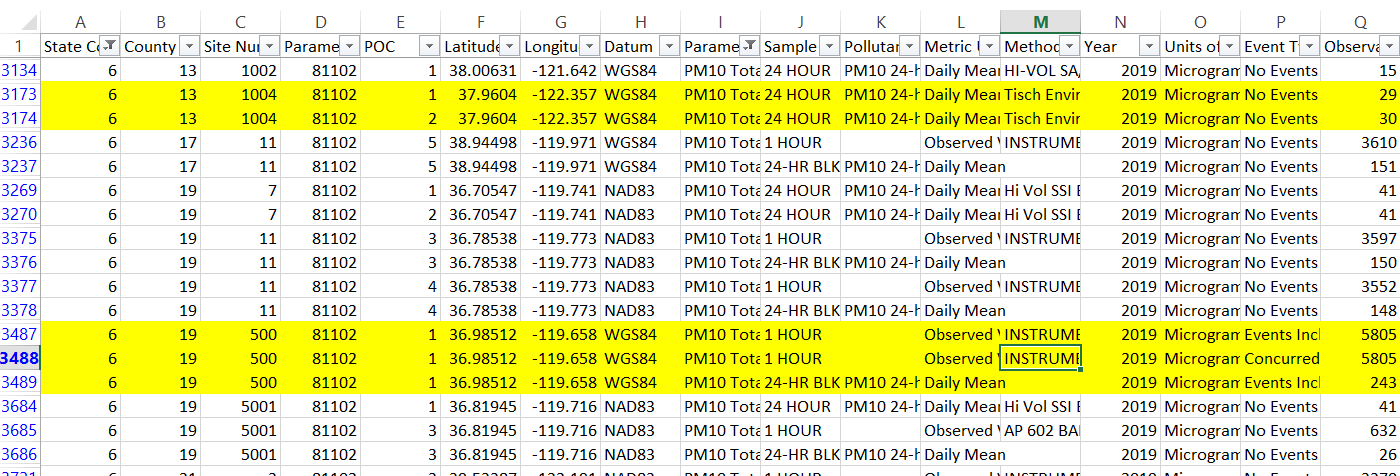
\includegraphics[width = \textwidth]{Figures/Validation/Example_Raw_EPA_Data.png}
\caption{A selected screen capture showing part of the .csv data file from the EPA for the year 2019.  The first yellow highlight shows a site with two \ac{FRM} \ac{POC} and no extreme events.  The lower yellow highlight shows a site with a single \ac{FEM} sensor that has extreme events and has, in the third highlighted row, been smoothed from hourly averages to daily averages.  Columns A-C defines a unique site, Column E shows the \ac{POC}, Column J the sample averaging period, Column P whether extreme events are included}
\label{fig:Example_Raw_EPA_Data}
\end{figure}

\subsubsection*{Data Columns}
\label{subsubsec:datacolumns}
Each of the \ac{EPA}'s annual summary files is a .csv with 55 columns, as described in table \ref{table:data_column_headers}.  The data columns include the Arithmetic Mean as well as the 99\ts{th}, 98\ts{th}, 95\ts{th}, 90\ts{th}, 75\ts{th}, 50\ts{th}, and 10\ts{th} Percentiles of all the observations made at that site by that instrument and for that pollutant.  For this report, the arithmetic mean 
was used as the statistic.  

In addition to the main data file, a .csv file containing metadata for each site was used. Its columns are outlined in table \ref{table:metadata_column_headers}.

%\afterpage{
%\clearpage % Flush earlier floats (otherwise order might not be correct)
%\thispagestyle{empty}% empty page style (?)
\begin{landscape}% Landscape page
	\begin{table}[ht]
		\centering
		\begin{tabular}{l | l | l | l | l }
			%{\textwidth}{c c X X X}
			\hline
			Site Identification & Pollutant Metadata & Observation Metadata & Data & Other Metadata  \\
			\hline
			State Number & Parameter Name & Year & Arithmetic Mean & Local Site Name \\
			County Number & Sample Duration & Units & Arithmetic Standard Deviation & Address \\
			Site Number & Pollutant Standard & Event Type & 1\ts{st} Max Value & State Name \\
			Parameter Code & Metric Used & Observation Count & 1\ts{st} Max Date Time & City Name \\
			\ac{POC} & Method Name & Observation Percent & ... & CBSA Name \\
			Latitude & & Completeness Indicator & ... & Date of Last Change \\
			Longitude & & Valid Day Count & 4\ts{th} Max Value & \\
			Datum & & Required Day Count & 4\ts{ts} Max Date Time & \\
			& & Exceptional Data Count & 1\ts{st} Max Non Overlapping Value & \\
			& & Null Data Count & 1\ts{st} Max Non Overlapping Date Time & \\
			& & Primary Exceedance Count & 99\ts{th} Percentile & \\
			& & Secondary Exceedance Count & 98\ts{th} Percentile & \\
			& & Certification Indicator & 95\ts{th} Percentile & \\
			& & Number of Observations below MDL & 90\ts{th} Percentile & \\
			& & & 75\ts{th} Percentile & \\
			& & & 50\ts{th} Percentile & \\
			& & & 10\ts{th} Percentile & \\
			\hline
		\end{tabular}
		\caption{Names of all the column headers in a raw data file containing annual air pollution data from the \ac{EPA}. Column headers are organized by general category and then listed in order of appearance.  So State Number is the 1\ts{st} column, County Number is the 2\ts{nd} and Parameter Name is the 9\ts{th}.  The exact definitions of each column can be found at the \ac{EPA} website: \url{https://aqs.epa.gov/aqsweb/airdata/FileFormats.html\#_content_3}}
		\label{table:data_column_headers}
	\end{table}
\end{landscape}

%\clearpage
%}
\begin{table}[ht]
\centering
\begin{tabular}{l|l|l|l}
	\hline
	State Code & Latitude & First Year of Data &  Networks\\
	County Code & Longitude & Last Sample Date &  Reporting Agency\\
	Site Number & Datum & Monitor Type & PQAO\\
	Parameter Code & & & Collecting Agency\\
	Parameter Name & & & Exclusions\\
	POC & & & Monitoring Objective\\
	& & & Last Method Code \\
	Local Site Name & & & Last Method \\
	Address & & & NAAQS Primary Monitor \\
	State Name & & & QA Primary Monitor \\
	County Name & & & \\
	City Name & & & \\
	CBSA Name & & & \\
	Tribe Name & & Extraction Date & \\
\end{tabular}
\caption{Names of column headers in metadata file describing the particulars of each site.  Full details on the \ac{EPA} website \url{https://aqs.epa.gov/aqsweb/airdata/FileFormats.html\#_format_2}}
\label{table:metadata_column_headers}
\end{table}

\subsection{Data Description}
\label{subsec:datadescripion}
\begin{figure}[ht]
\centering
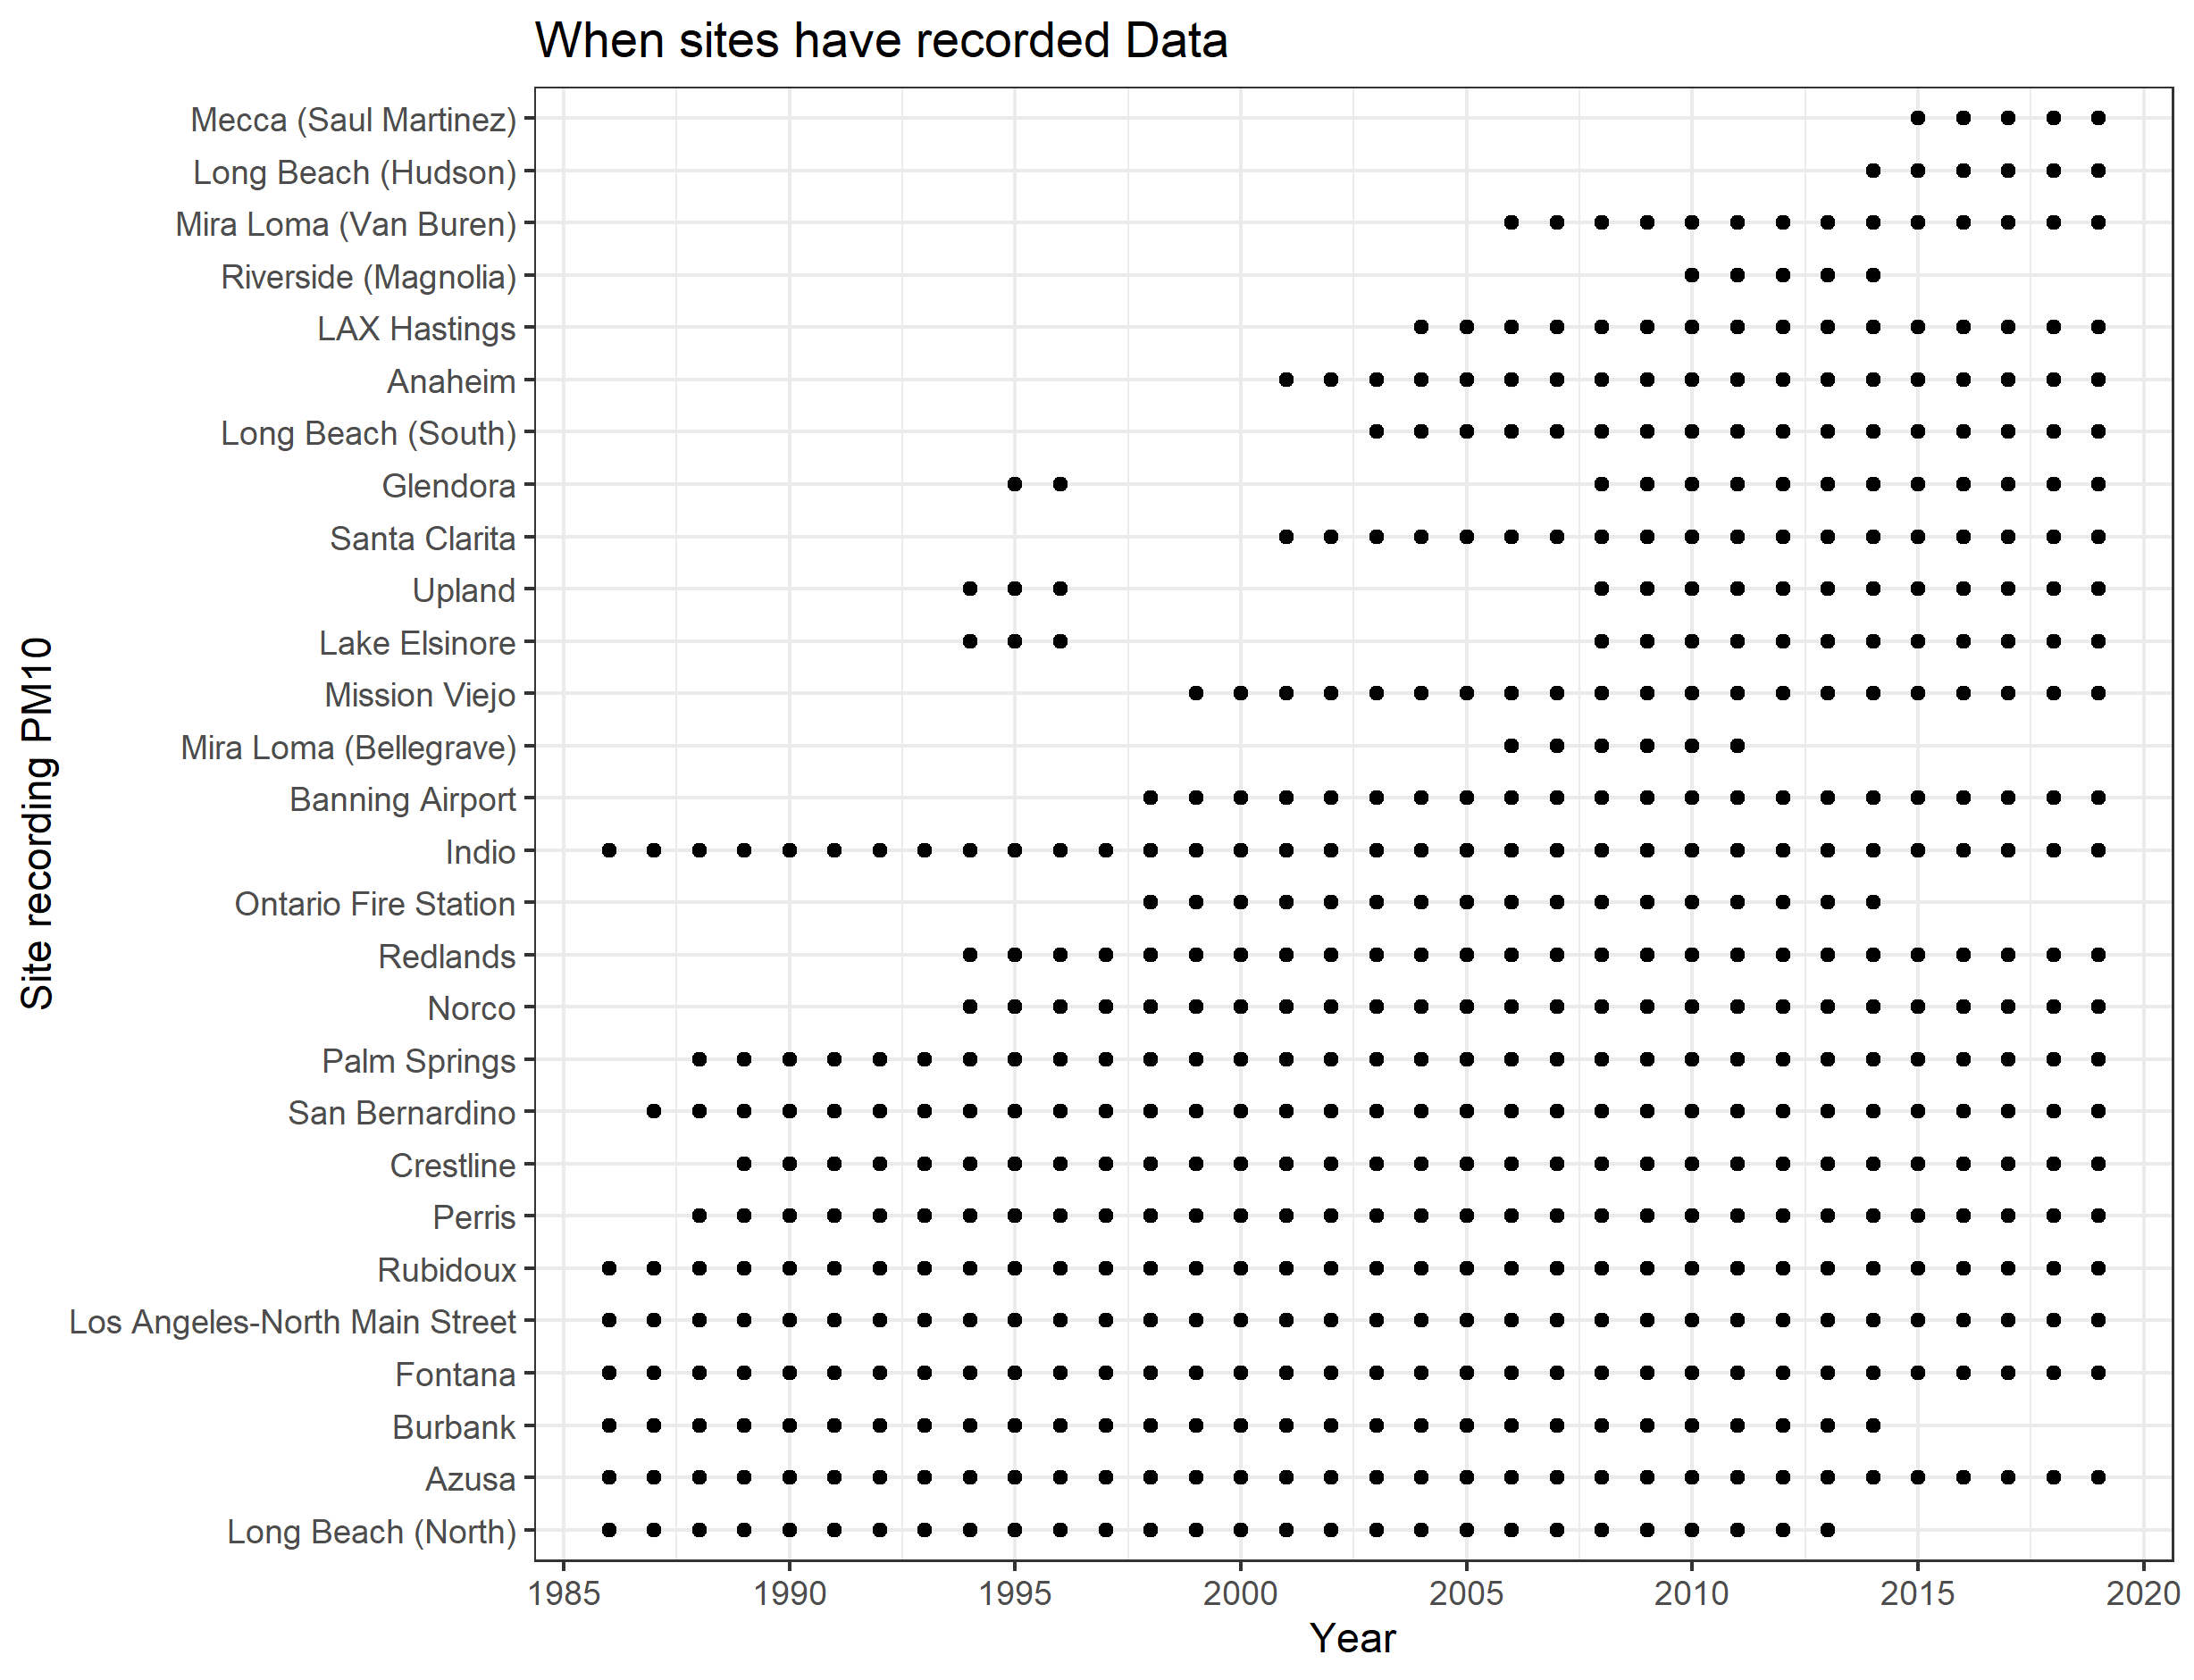
\includegraphics[width = \textwidth]{Figures/site_dotplot-colour.png}
\caption{This figure shows how the network developed over time.  We can see that sites are generally added to the network, that 5 sites have been removed, and that 5 sites started in 1986.  A handful of sites exhibit the unusual behaviour of being taken offline and then removed.  These are sites that only had \ac{FRM} monitoring, no \ac{FEM}.}
\label{fig:site_dotplot}
\end{figure}

\begin{figure}[ht]
\centering
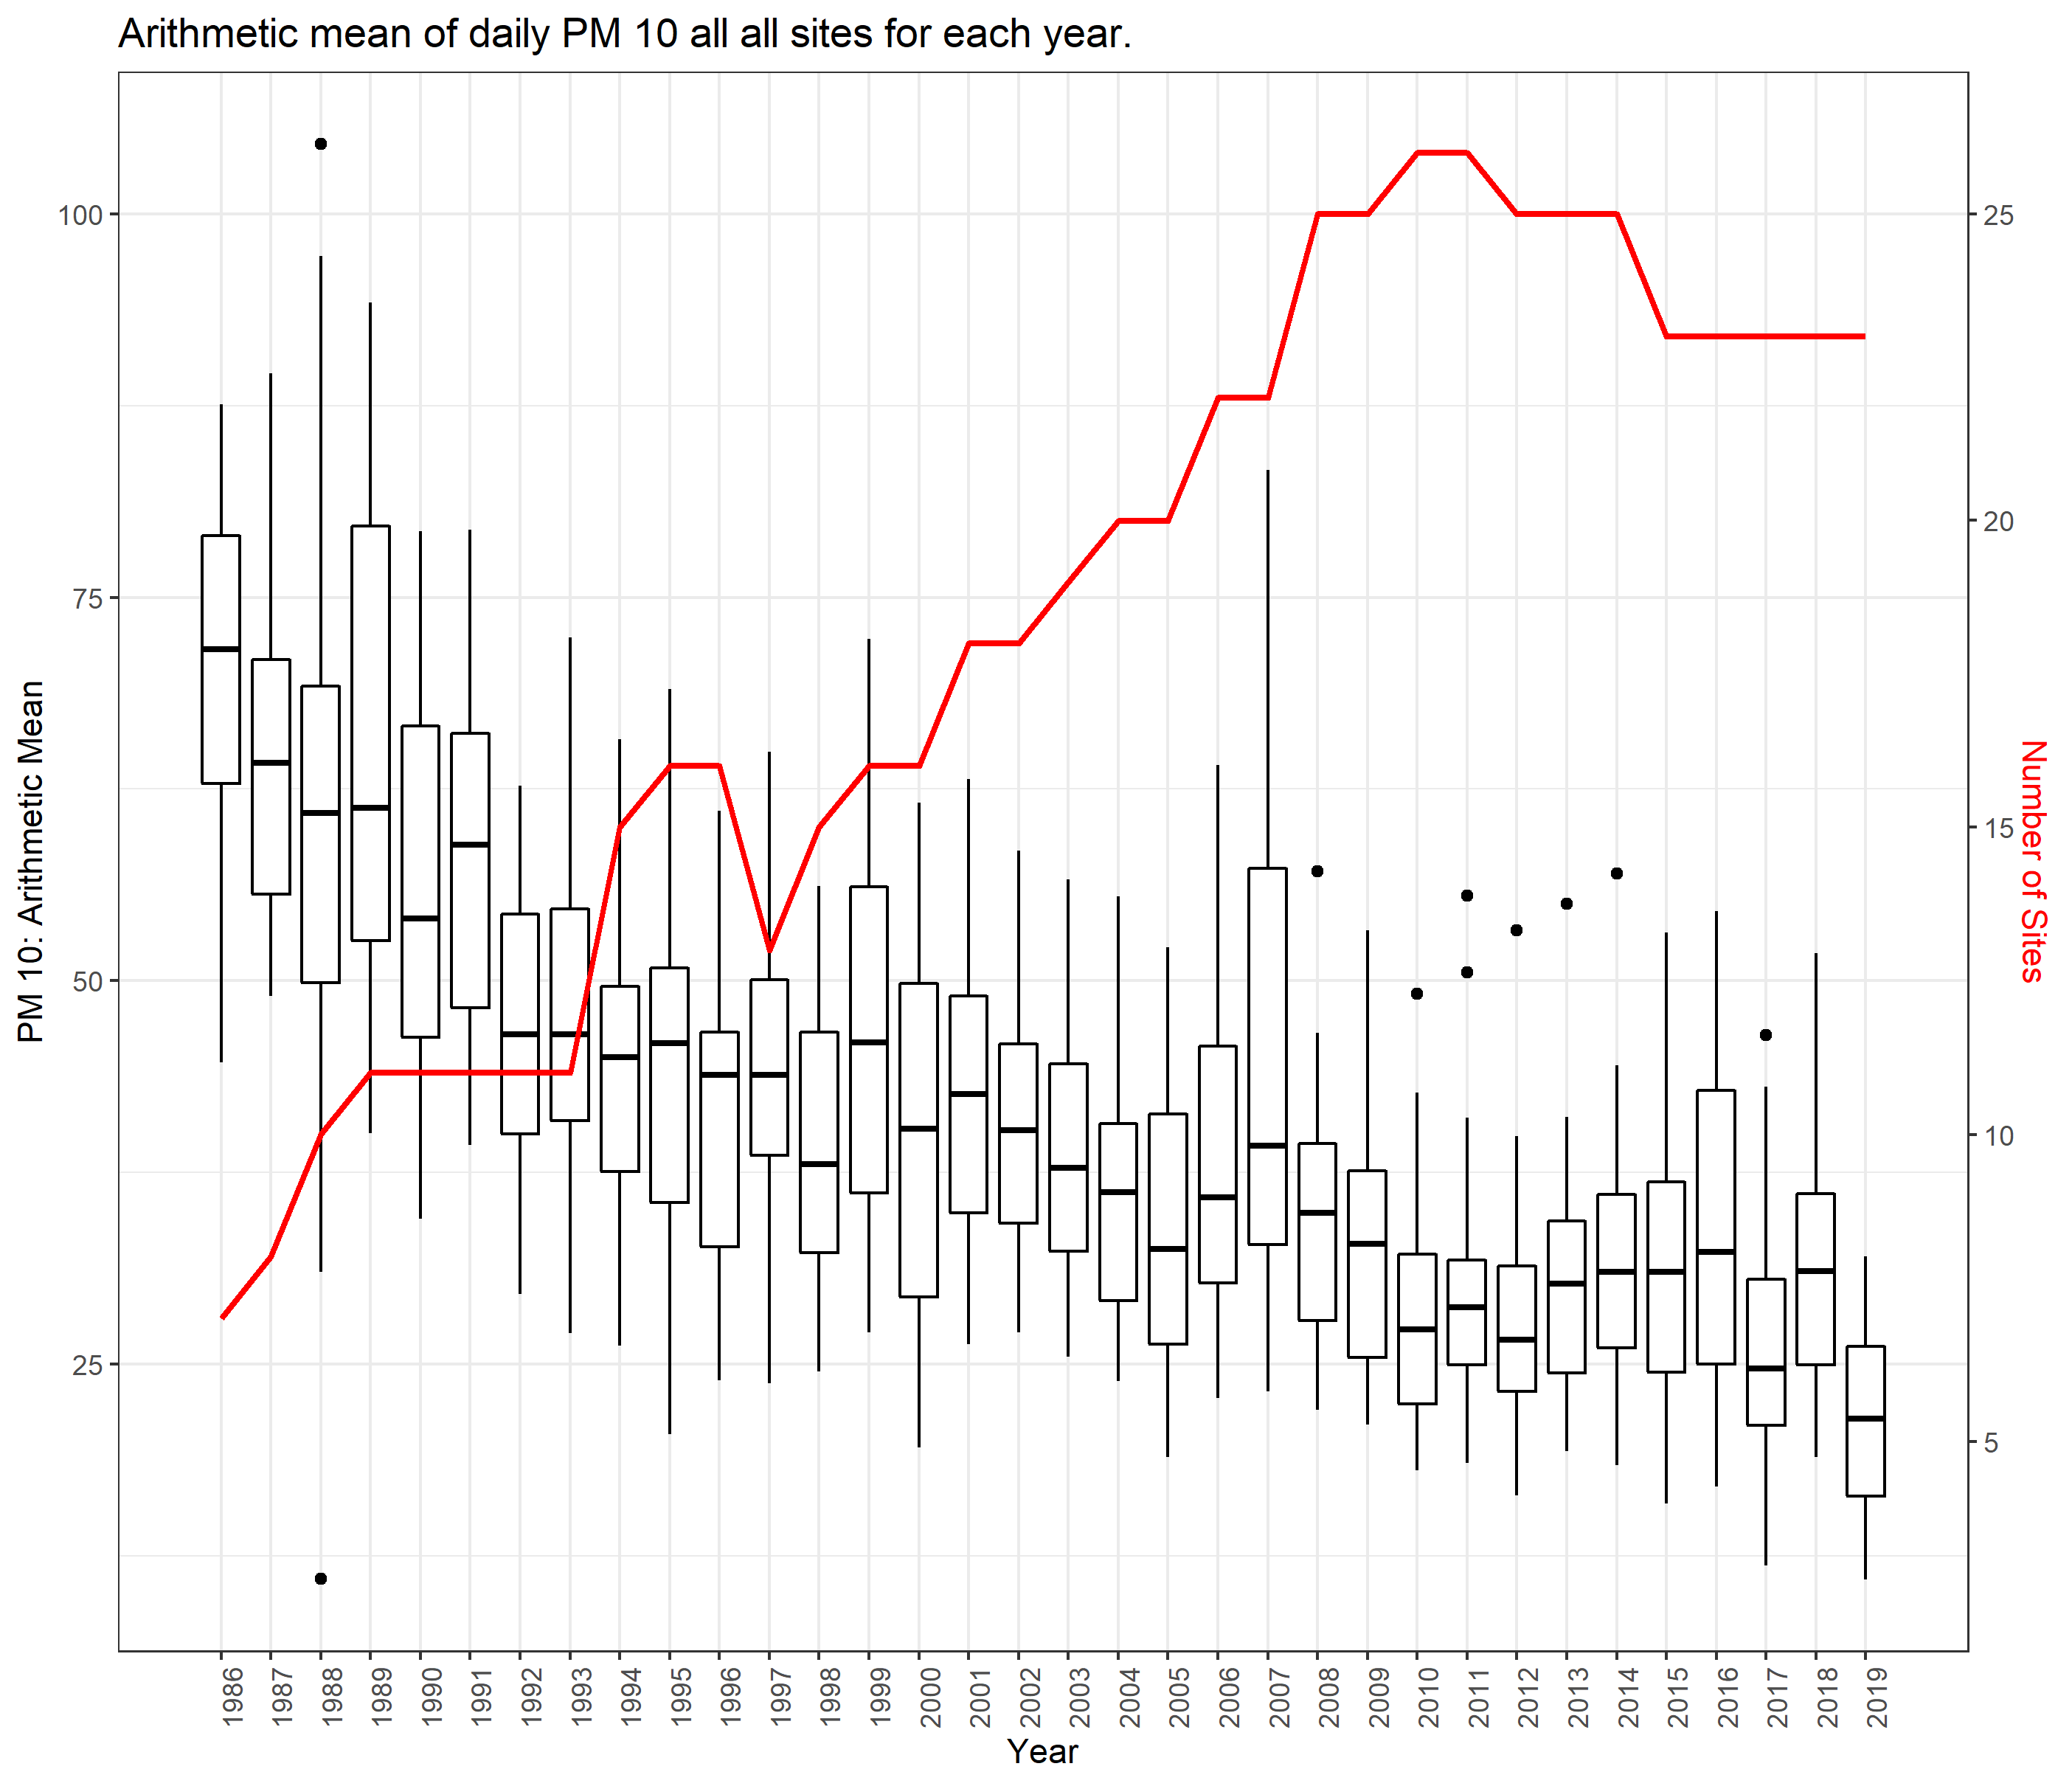
\includegraphics[width = \textwidth]{Figures/site_trend-ArthmM_NumSites.png}
\caption{Each box shows the general pattern of mean 
	PM10 is observed each year.  The red line shows how the number of active sites recording in the network (and therefore the number of observations feeding into each box) increases to the present day.}
\label{fig:site_trend-ArthmM_NumSites}
\end{figure} 

From 1986 to 2019 there are 28 unique sites monitoring \ac{PM10} within the \ac{SOCAB}. Figure \ref{fig:site_dotplot} shows when sites are included in the network and when they are removed.   Three sites (Glendora, Upland and Lake Elsinore) stopped being recorded in 1997 and then restarted in 2008. Why this happens, is unclear, but it only occurs in sites with only continuous \ac{FEM} monitoring (as opposed to scheduled \ac{FEM} sampling).  The timeline coincides with regulatory changes to standards, but we have been unable to learn the reason for the sites' discontinuation and restart.

Figure \ref{fig:site_trend-ArthmM_NumSites} summarizes the yearly mean \ac{PM10} and shows how, over time, the number of sites has increased while the overall concentration in the area has gone down. The trend in \ac{PM10} will be examined later. 

\subsubsection*{Network Trends}
\label{subsubsec:networktrends}
Here are several plots showing traces of each site compared to the rest of the network.  If the network is being biased consistently over time towards a certain goal, we would expect to see some difference between sites kept in the network vs those removed from it.  

\begin{figure}[ht]
\centering
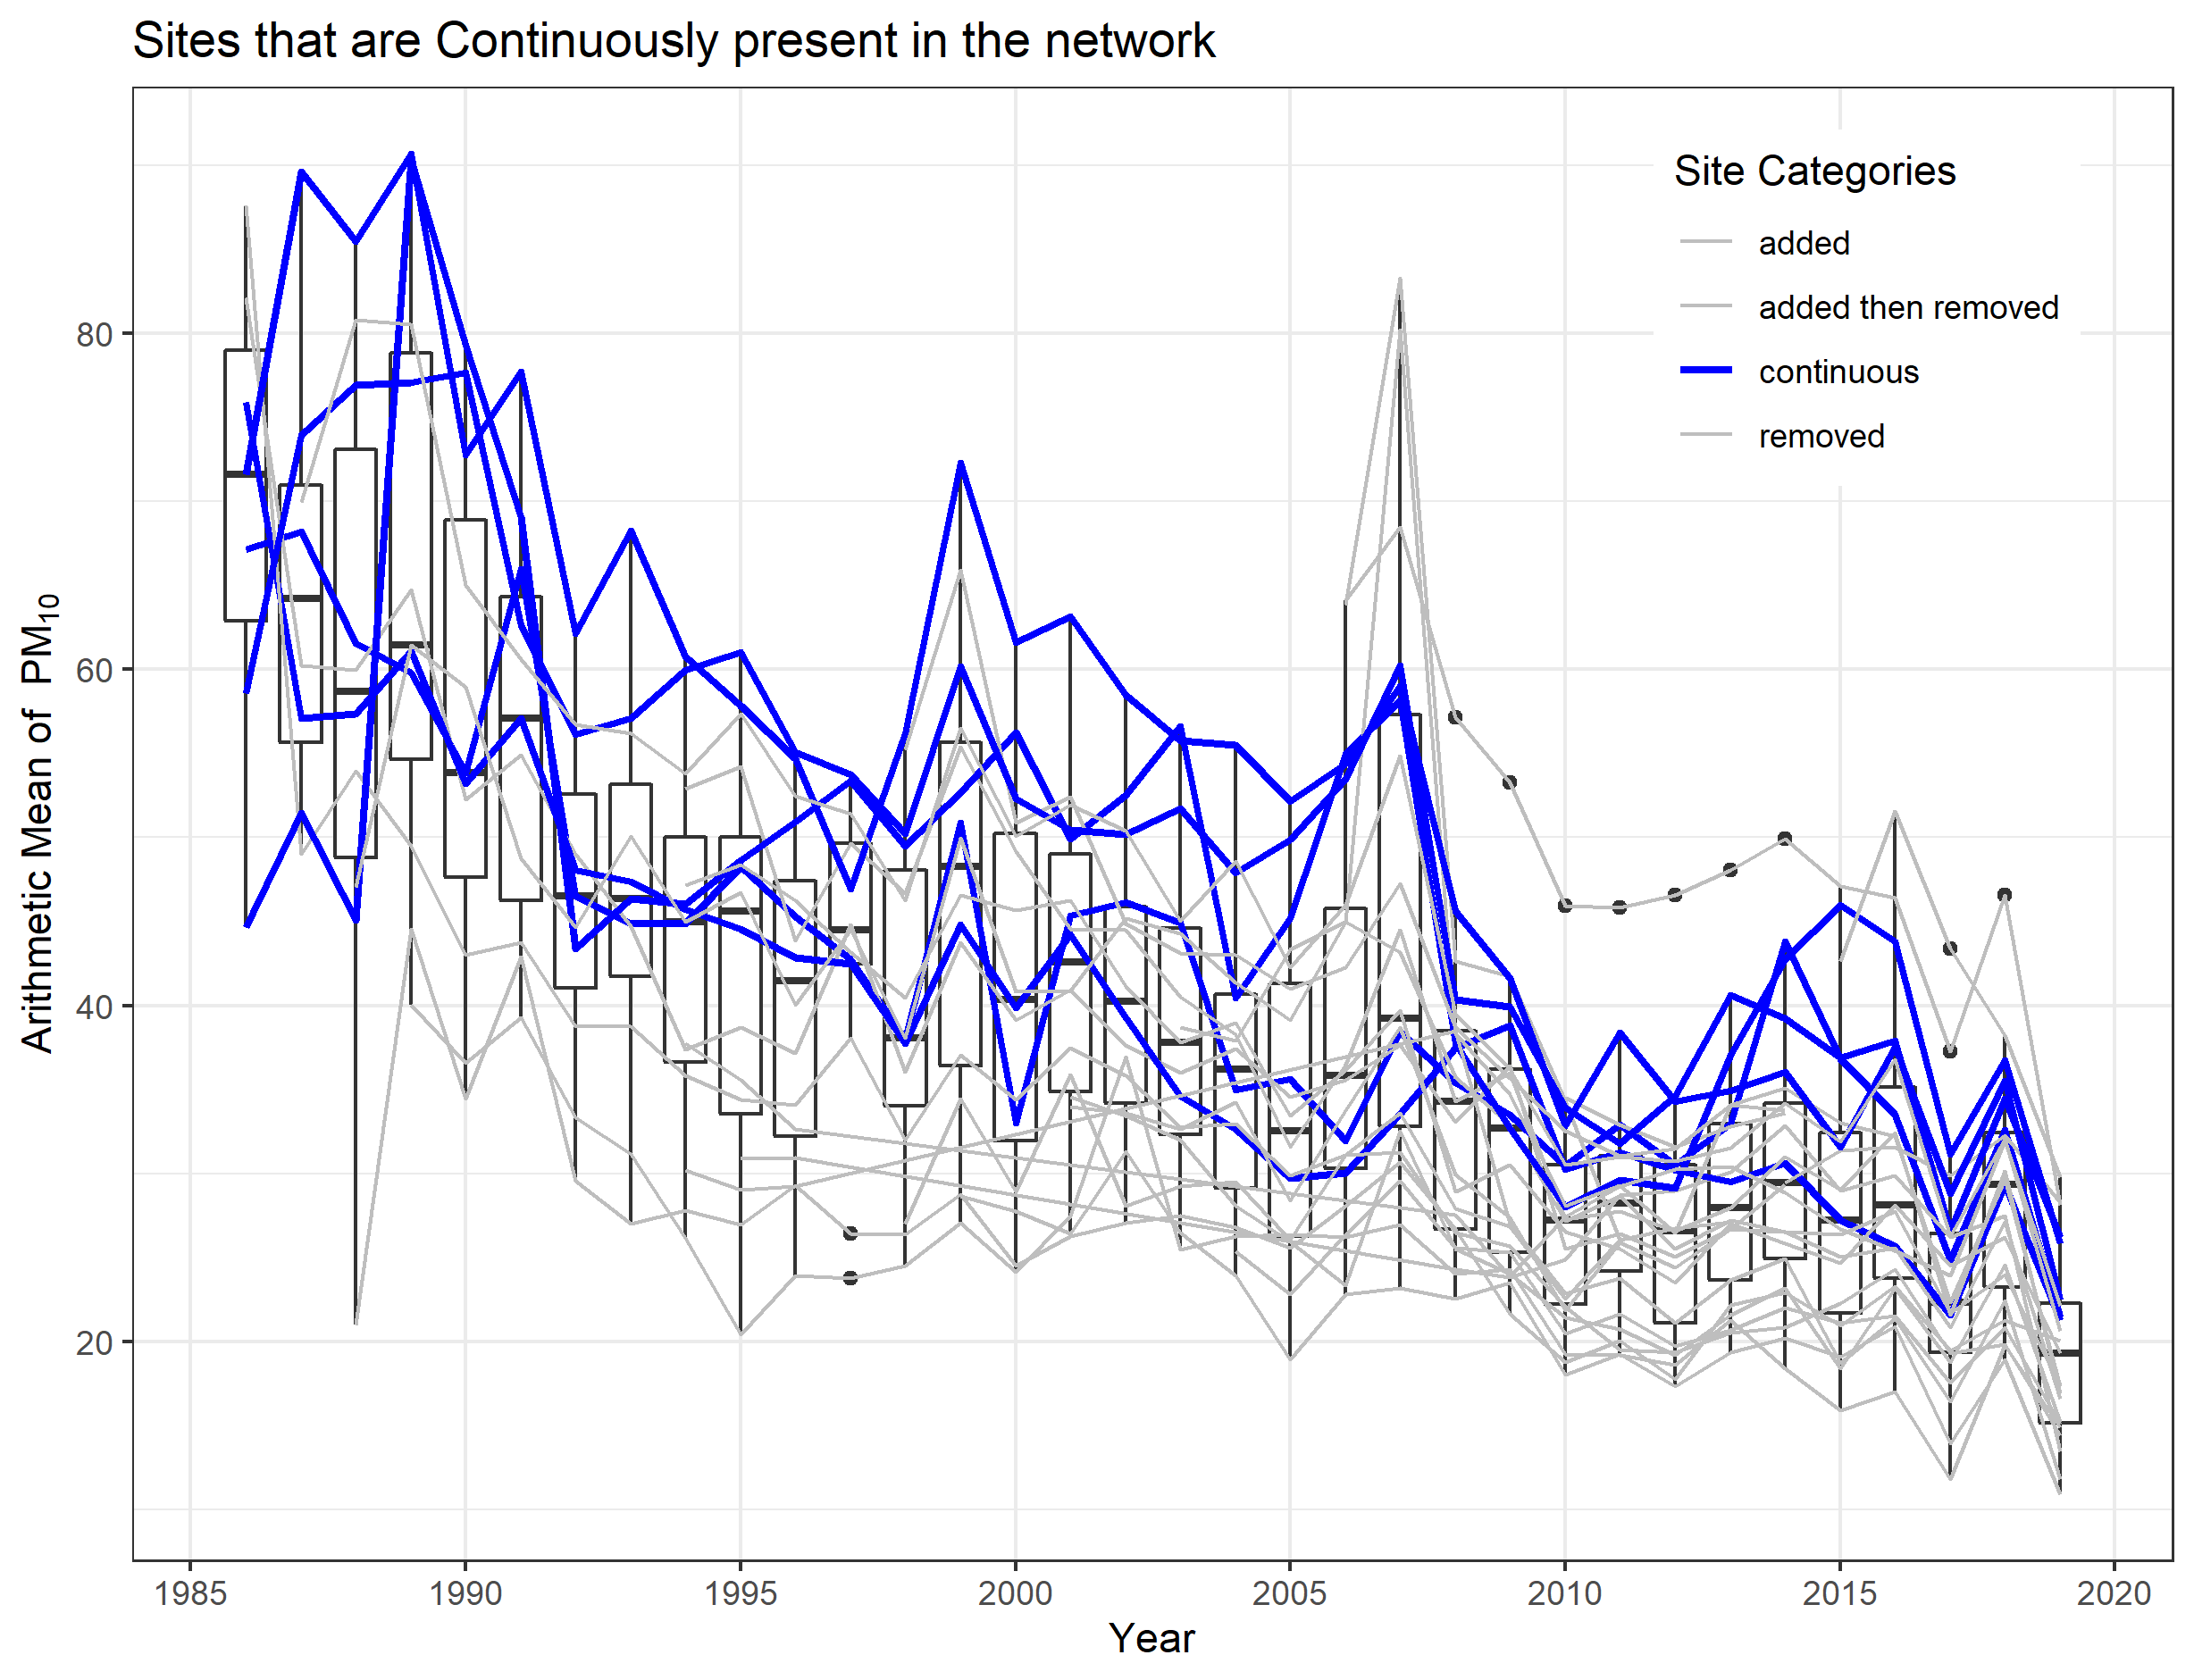
\includegraphics[width = \textwidth]{Figures/site_timing_trace-Continuous.png}
\caption{This figure highlights the traces of all the sites that started in the network and have not been removed.  We can see that in later years the lower part of the boxes is not covered by these traces, indicating some possibility of preferential sampling.  In the case when a site had multiple \ac{POC} in a year, the value at the trace is the mean of all \ac{POC} at that site for that year.}
\label{fig:site_timing_trace-Continuous}
\end{figure}
Figure \ref{fig:site_timing_trace-Continuous} shows the sites that are active from 1986 to the present day, labelled as continuously present.  The continuously present sites tend to be above the mean in more recent years.  If sites maintain their relative position in the overall distribution, this suggests the early years are biased towards higher sites.

\begin{figure}[ht]
\centering
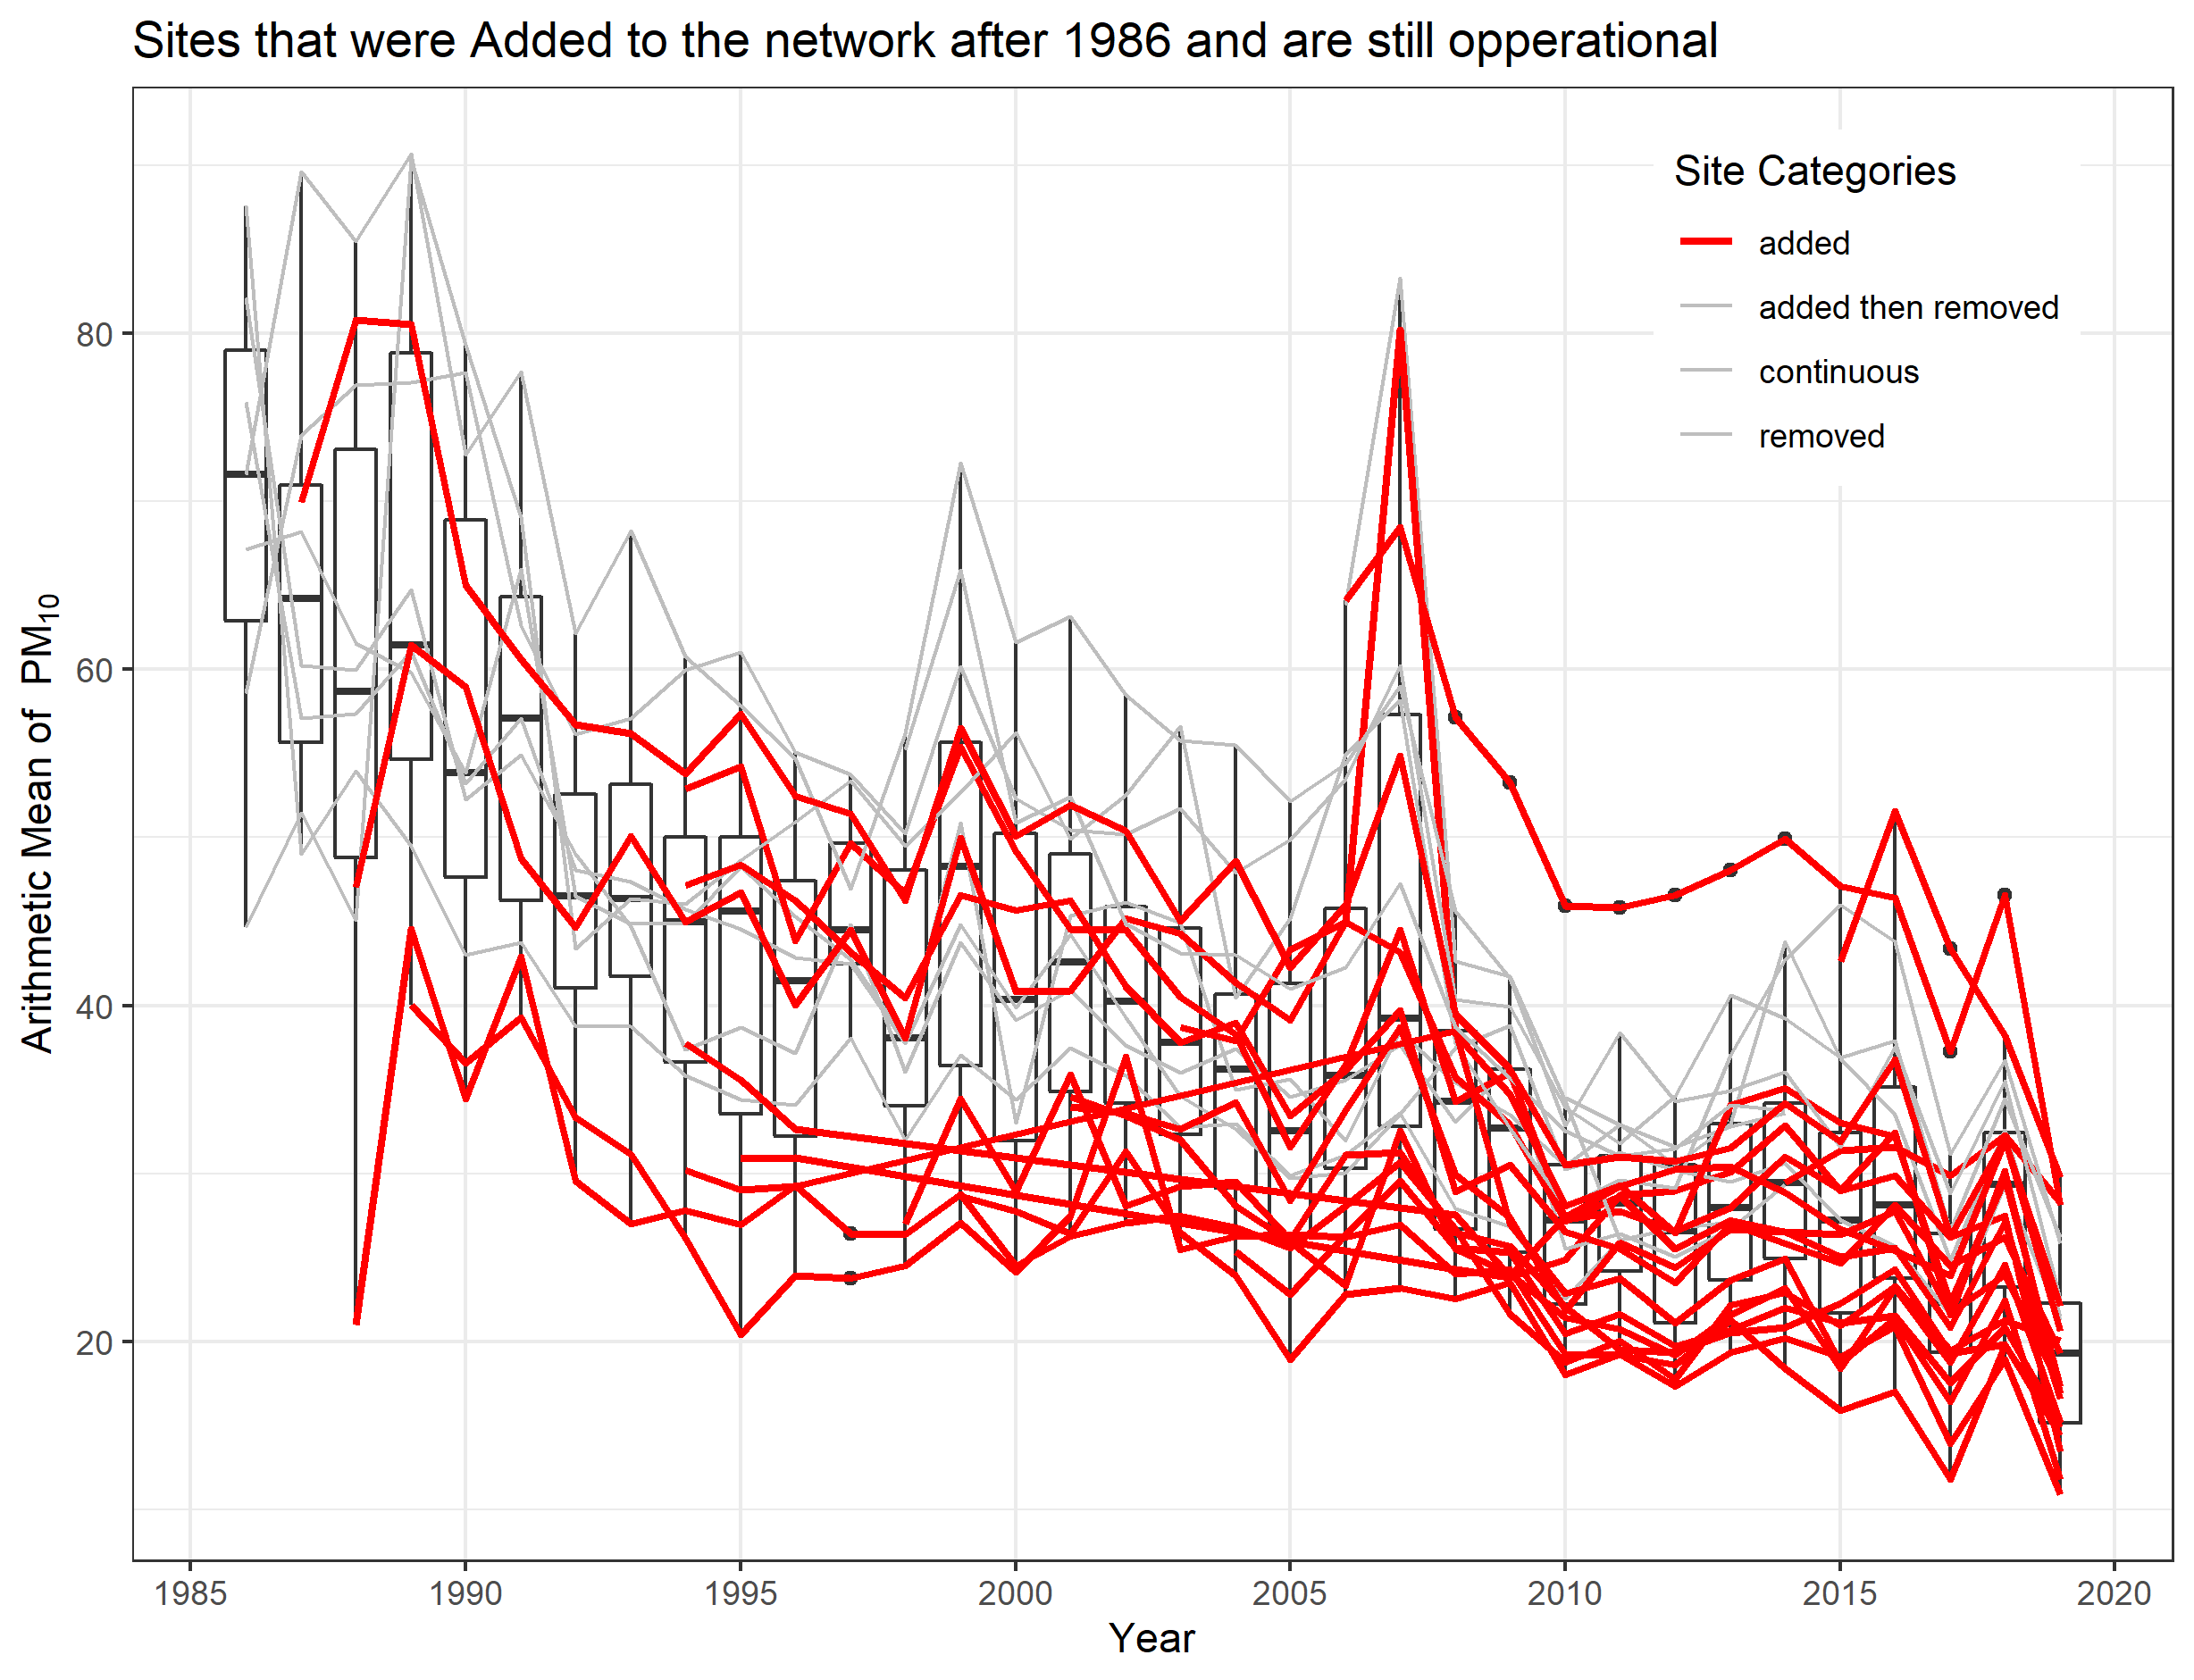
\includegraphics[width = \textwidth]{Figures/site_timing_trace-Added.png}
\caption{Here are highlights of all the sites that were added after 1986.  It appears that there are more traces in the lower portion of the boxes, which is the required complement of the pattern shown in the previous figure.  Again, in the case when a site had multiple \ac{POC} in a year, the value at the trace is the mean of all \ac{POC} at that site for that year.}
\label{fig:site_timing_trace-Added}
\end{figure}

Figure     \ref{fig:site_timing_trace-Added} shows how sites added to the network tend to fill out the bottom half of the distribution in later years. This is the inverse of the idea demonstrated in the previous figure (Figure  \ref{fig:site_timing_trace-Continuous}).

\begin{figure}[ht]
\centering
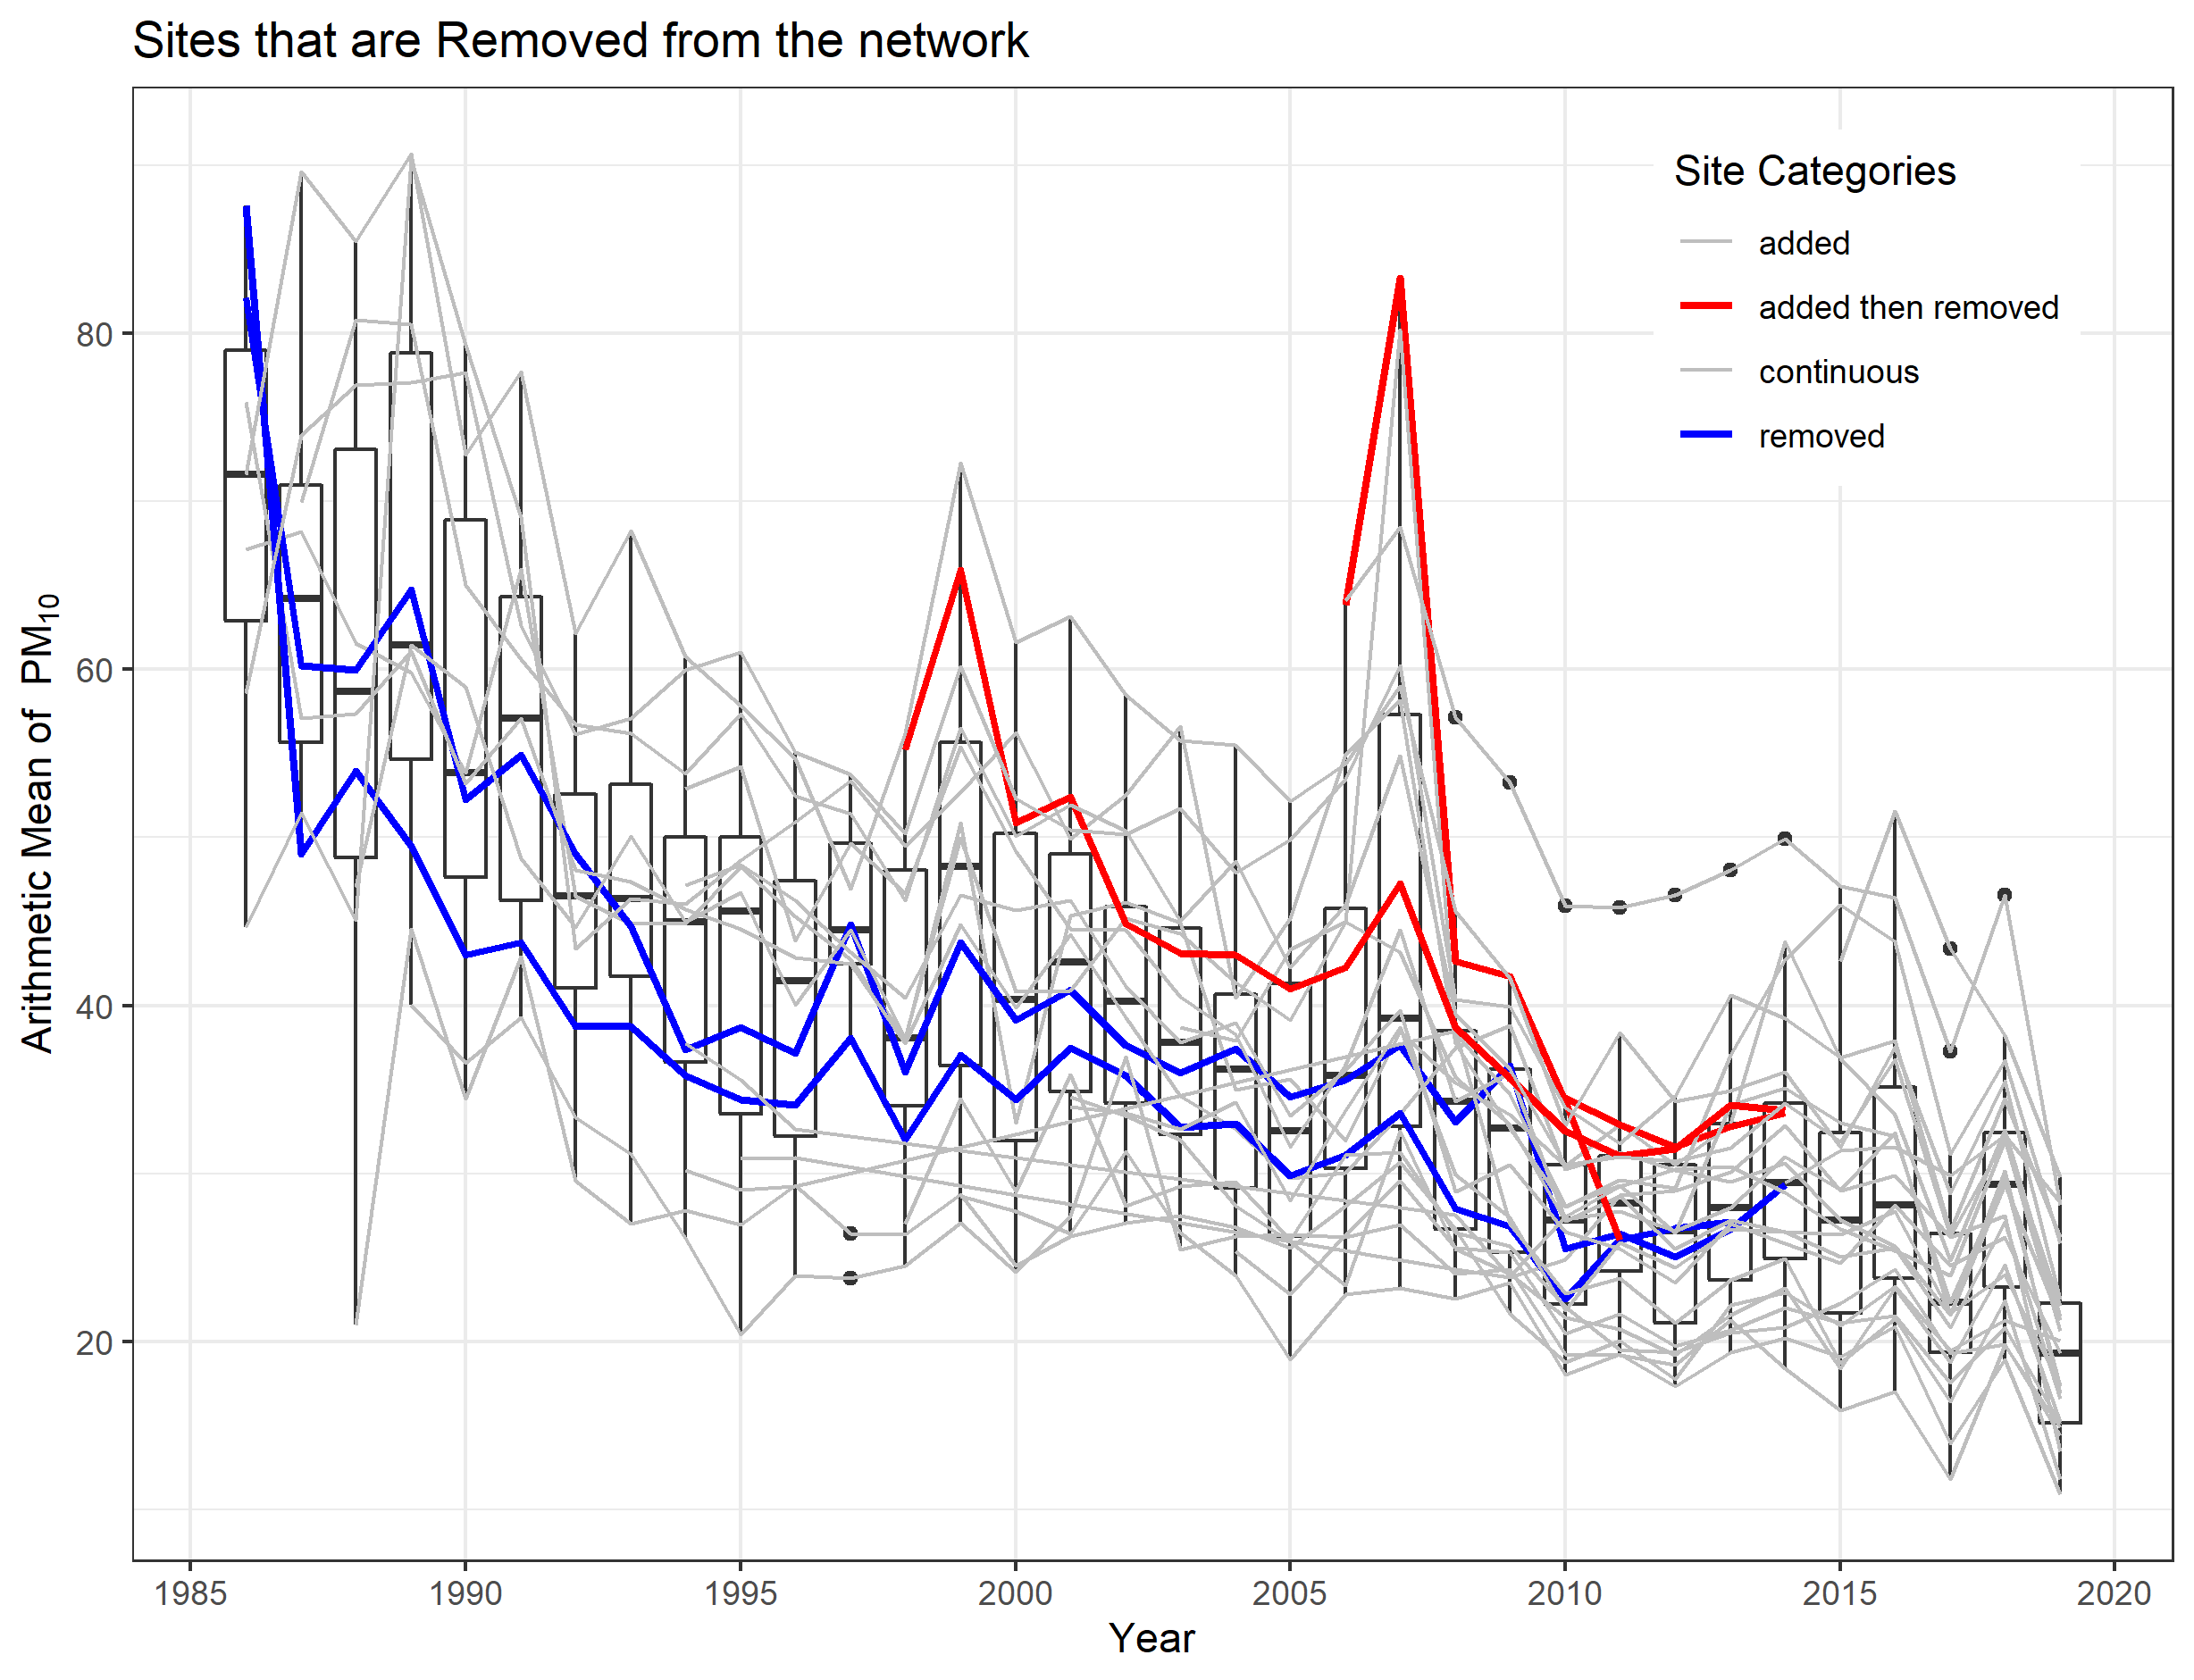
\includegraphics[width = \textwidth]{Figures/site_timing_trace-Removed.png}
\caption{This figure highlights the sites that were dropped from the network.  In Blue are two sites that started in 1986 but were then removed.  In Red are three sites that were added to the network after 1986 and have been since removed.  }
\label{fig:site_timing_trace-Removed}
\end{figure}
Figure  \ref{fig:site_timing_trace-Removed} highlights the five sites that were dropped from the network.  Two of them were part of the original network in 1986, and tend to fall below the yearly mean.   The other three were added to the network and tend to be above the yearly mean.  This behaviour is opposite to that seen in the plots of continuous sites and sites that were added and kept.  The sites that start in the network in 1986 and remain throughout tend to be above the mean, but the two that were removed are below the mean.  The sites that were added to the network tend (to a lesser degree) to be below the mean, but those that were added and then removed tend to be above it.

\subsubsection*{Site Location}
\label{subsubsec:sitelocn}
Figure  \ref{fig:SOCAB_counties} shows the location of sites in the \ac{SOCAB}.  Note that they are not all present simultaneously.  
%Appendix B has figures showing the site locations for each year.  
It appears that some sites replace others.  For example, Long Beach (North) and Long Beach (Hudson) are very close to each other and one stops while the other starts the next year.  This lack of Independence in site selection was ignored.

\begin{figure}[ht]
\centering
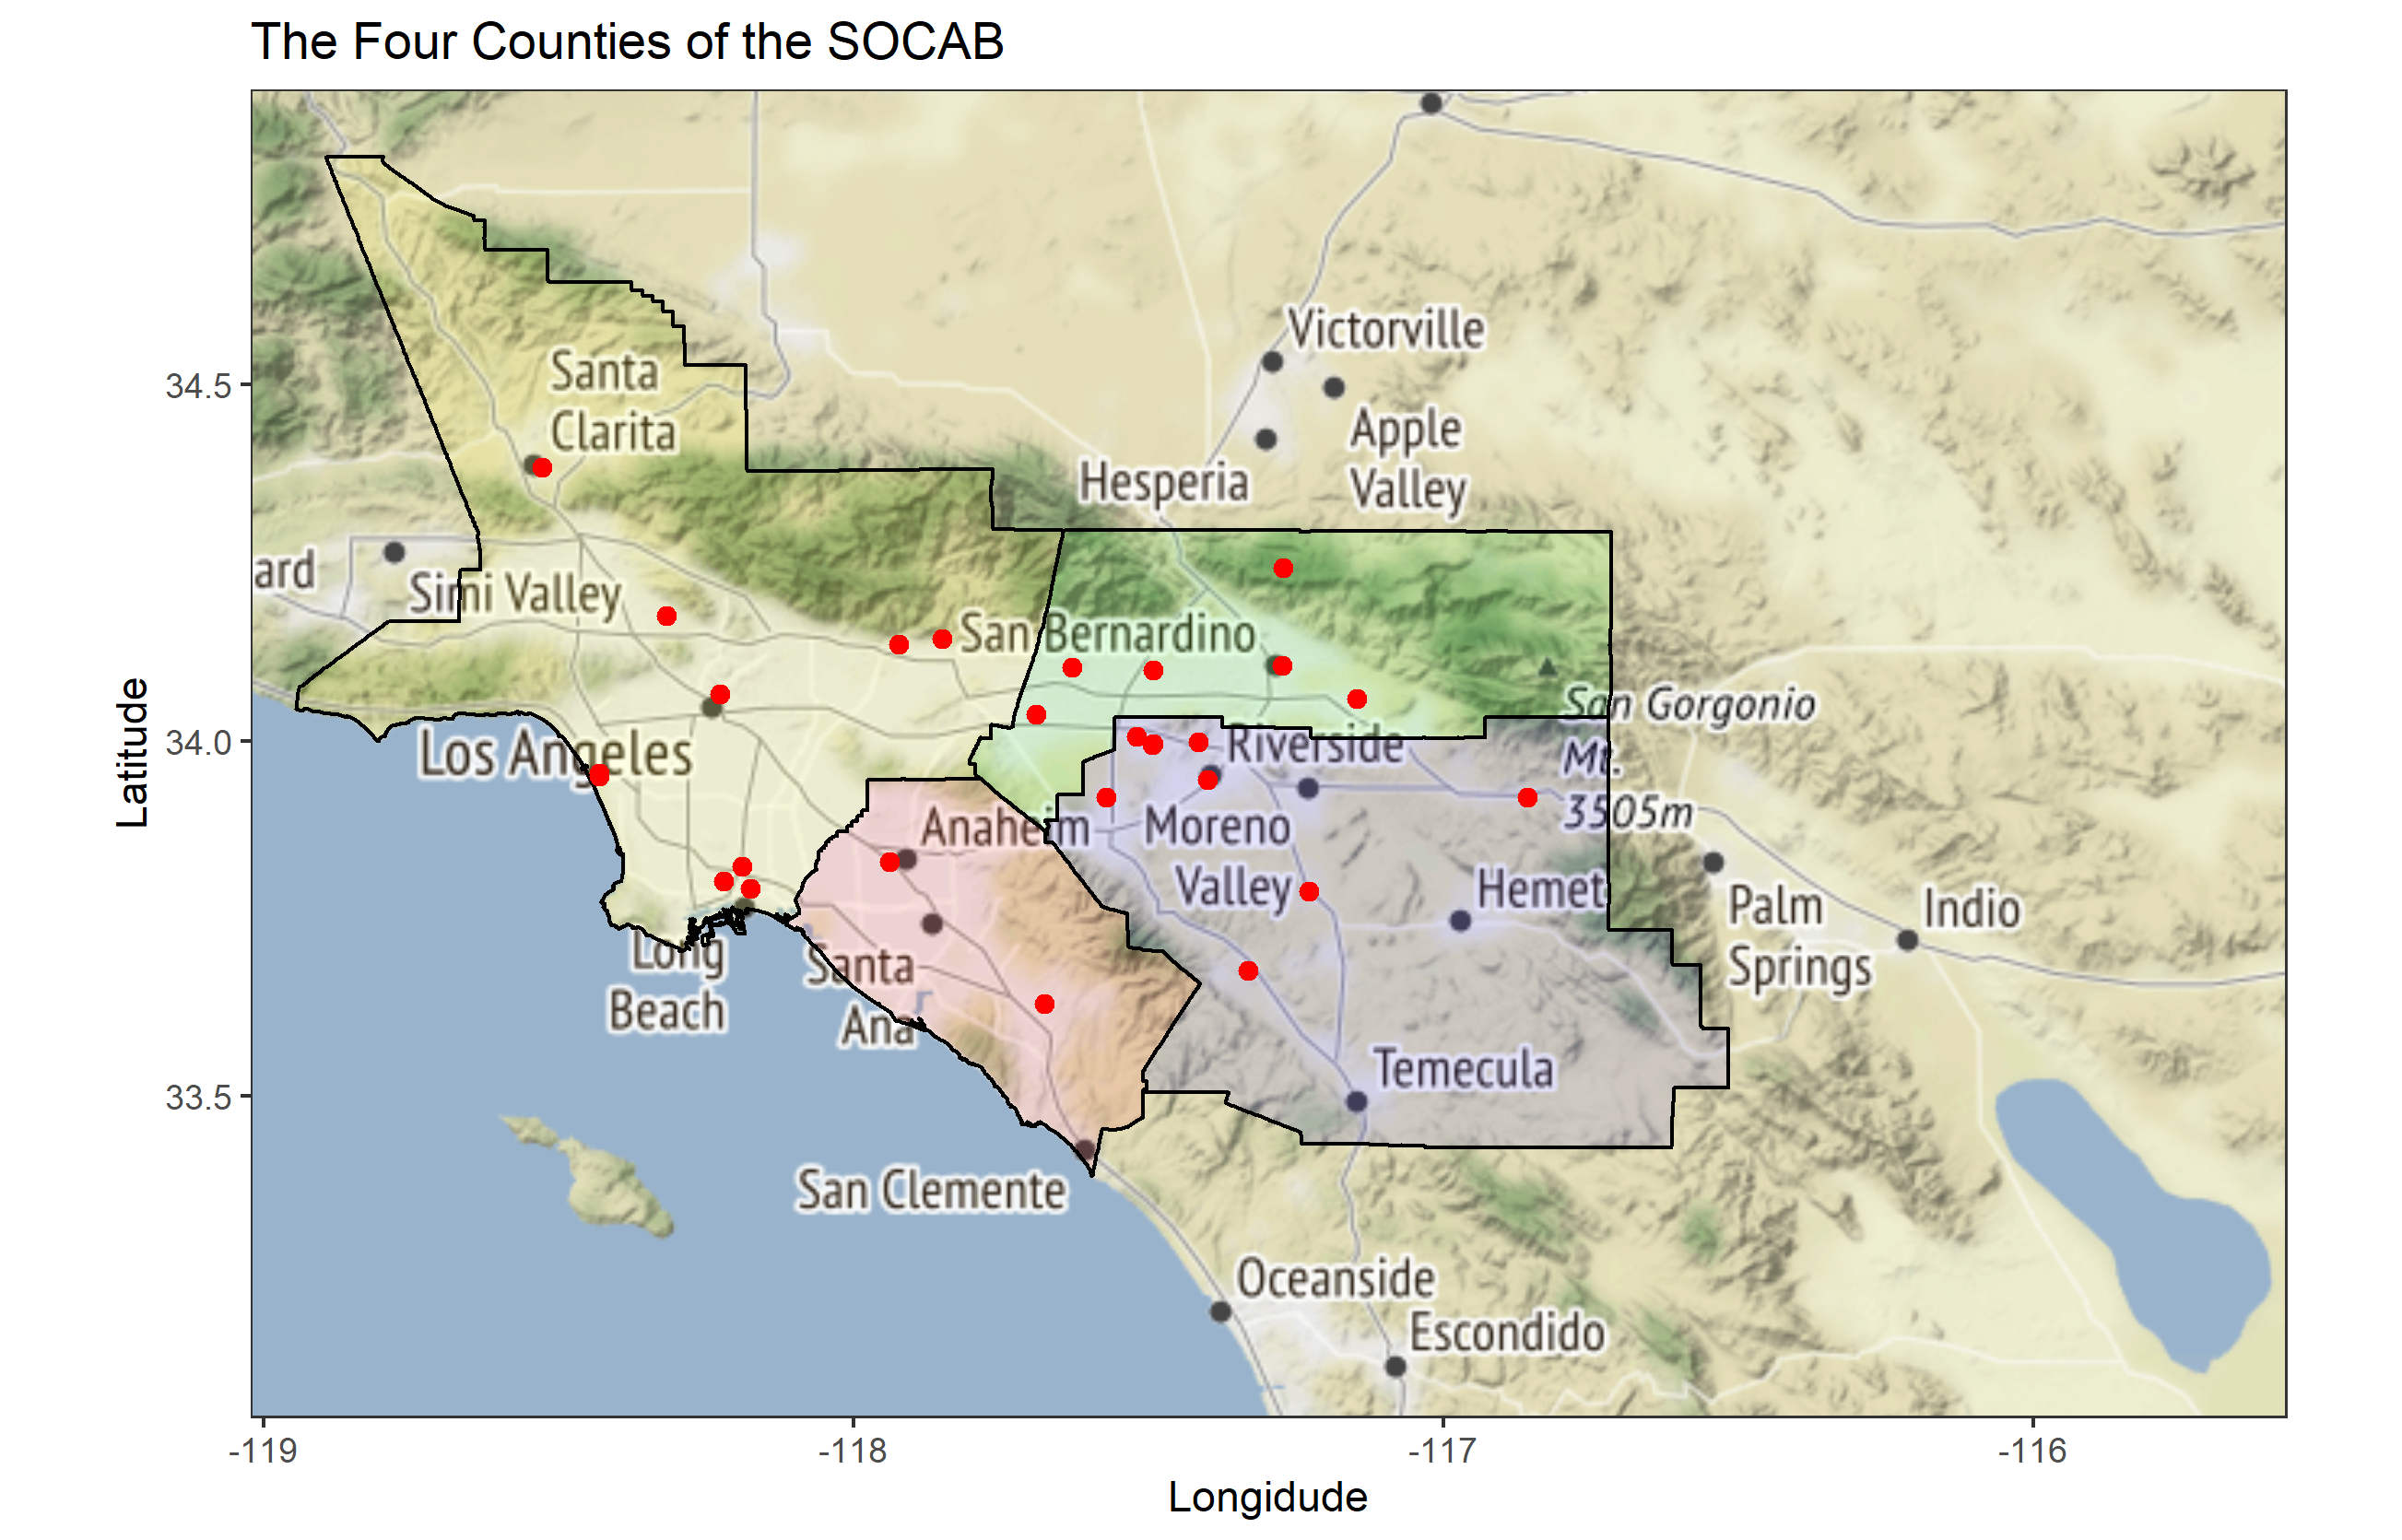
\includegraphics[width = \textwidth]{Figures/SOCAB_counties.png}
\caption{This map shows the \ac{SOCAB} about the Los Angeles region.  It includes 4 counties, Orange County (Pink), Los Angeles County (Yellow), Riverside County (Blue), and San Bernardino County (Green).  Only Orange County is entirely part of the \ac{SOCAB} and the other counties extend into other air basins.  Monitoring sites that are included in this study are red dots.}
\label{fig:SOCAB_counties}
\end{figure}

\subsubsection*{Site Metadata}
\label{subsubsec:sitemetadata}
The \ac{EPA} and \ac{SCAQMD} record additional descriptive information about each site.  This includes:  

\begin{itemize}
\item \textbf{Land Use:} Figure  \ref{fig:SOCAB_metadata_Site_Land_use} shows the Land Use, describing whether the site is residential, commercial, industrial, or agricultural.  Most (17) sites are residential, 3 sites are Industrial, 6 sites are Commercial, 1 is Agricultural, and Indio (a site that started in 1986 and never dropped) has no stated land use.

\item \textbf{Location Setting:} Figure  \ref{fig:SOCAB_metadata_Site_Status} shows the Location Setting, describing whether the site is Urban (7 sites), Suburban (19 sites), or Rural (2 sites).  Interestingly, the rural and suburban bracket the urban making a sandwich.  

\item \textbf{Monitoring Objective:} Figure  \ref{fig:SOCAB_metadata_Site_Type} shows the Monitoring Objective, describing what the site is recording.  Options include Extreme Downwind, Highest Concentration, Other, Population Exposure, Unknown, and Upwind Background.   
\end{itemize}

\subsubsection*{Monitoring Purposes}
\label{subsubsec:purposes}
Every site has at least one monitoring purpose.  Some sites have mismatched site categories between the two 5 year reports.  However, we have not been able to determine if these are typos (other, more clear-cut typos have been found in the report) or if different monitors at the same location have a different category for some reason.  Here are the sites that mismatch:

\begin{itemize}
\item San Bernardino (\#060719004) is categorized as High Concentration except for the 2010 continuous monitor which is Population Exposure
\item LAX Hastings (\#060375005) is categorized as Population Exposure and Population Exposure / Background in 2015
\item Palm Springs (\#060655001) is categorized as High Concentration except for 2010s FEM monitor which is Population Exposure.
\end{itemize}

The site category was only High Concentration and Population Exposure categories (LAX Hastings being the one exception, being both PE and HC in 2015 for the FEM sensors)

\begin{table}[ht]
\centering
\begin{tabular}{p{3cm}|p{2cm}||p{3cm}|p{2cm}}
	\multicolumn{2}{c|| }{\small 2010 (Monitoring Purpose)} & \multicolumn{2}{c}{\small 2015 (Monitoring Purpose)}   \\
	\hline  
	Long Description & { \small Two-Letter Code} & Long Description & { \small Two-Letter Code} \\
	\hline
	{ \small High Concentration} & HC & { \small Highest Concentration} & HC \\
	{\small Representative Concentration}  & RC & { \small Population Exposure} & PE  \\
	{ \small Impact}  & IM & { \small Source Orientated (impact) }& IM \\
	{ \small Background} & BK & { \small General Background  }& BK \\
\end{tabular}
\caption{Comparison of Terminology describing the category into which each site is placed for the 5-year summaries seen in Table 2 of the two summaries.}
\label{tab:site_cat_5yr_summary}
\end{table}

\begin{table}[ht]
\centering
\begin{tabular}{p{3cm}|p{2cm}||p{3cm}|p{2cm}}
	%\begin{tabular}{l|l||l|l}
	\multicolumn{2}{c|| }{2010 (Monitoring Purpose)} & \multicolumn{2}{c}{2015 (Monitoring Purpose)}   \\
	\hline  
	Long Description & Two-Letter Code & Long Description & Two-Letter Code \\
	\hline
	Background Level & BK & & BK \\
	High Concentration & HC & & HC \\
	Pollutant Transport  & TP & & TP \\
	Pollutant Exposure & EX & & EX \\
	Source Impact & SO & & SO \\
	Representative Concentration & RC & & RC \\
	Special Purpose Monitoring   & SPM & -- & -- \\
	Trend Analysis & TR & & TR \\
	Site Comparison & CP & & CP \\
	-- & -- & Real-time Monitoring and Reporting & RM \\
	-- & -- & Collocated & CO \\
\end{tabular}
\caption{Comparison of terminology describing the purpose of each site, as described in table 3 of the 2010 and 2015 5-year summaries.  Not all categories exist in both years, when one isn't present a--is placed in the year for which it is absent.}
\label{tab:monitoring_purpose_5yr_summary}
\end{table}

\subsubsection*{\ac{POC}} \label{seq:POC}
As discussed in Section \ref{subsubsec:DataRows} each site has at least one sensor, but many have more than one.  These could be an \ac{FEM} and a \ac{FRM} monitor, instrument changes, or collocation for trials or calibration.  This redundancy provides an interesting way to estimate the nugget effect, which is sensor uncertainty.  Figure  \ref{fig:POC_all_trace} shows traces for every \ac{POC} at each site.   An example of the instrument changes seems to happen in 1988 when all the sites that had been in operation before 1988 received at least one other \ac{POC} that returned a consistently higher reading of \ac{PM10} and the \ac{POC} that was in operation before 1988 was discontinued.  These sites are Azusa, Burbank, Fontana, Indio, Long Beach (North), Los Angeles-North, Palm Springs, Perris, Rubidoux, and San Bernardino.  

\begin{figure}[ht]
\centering
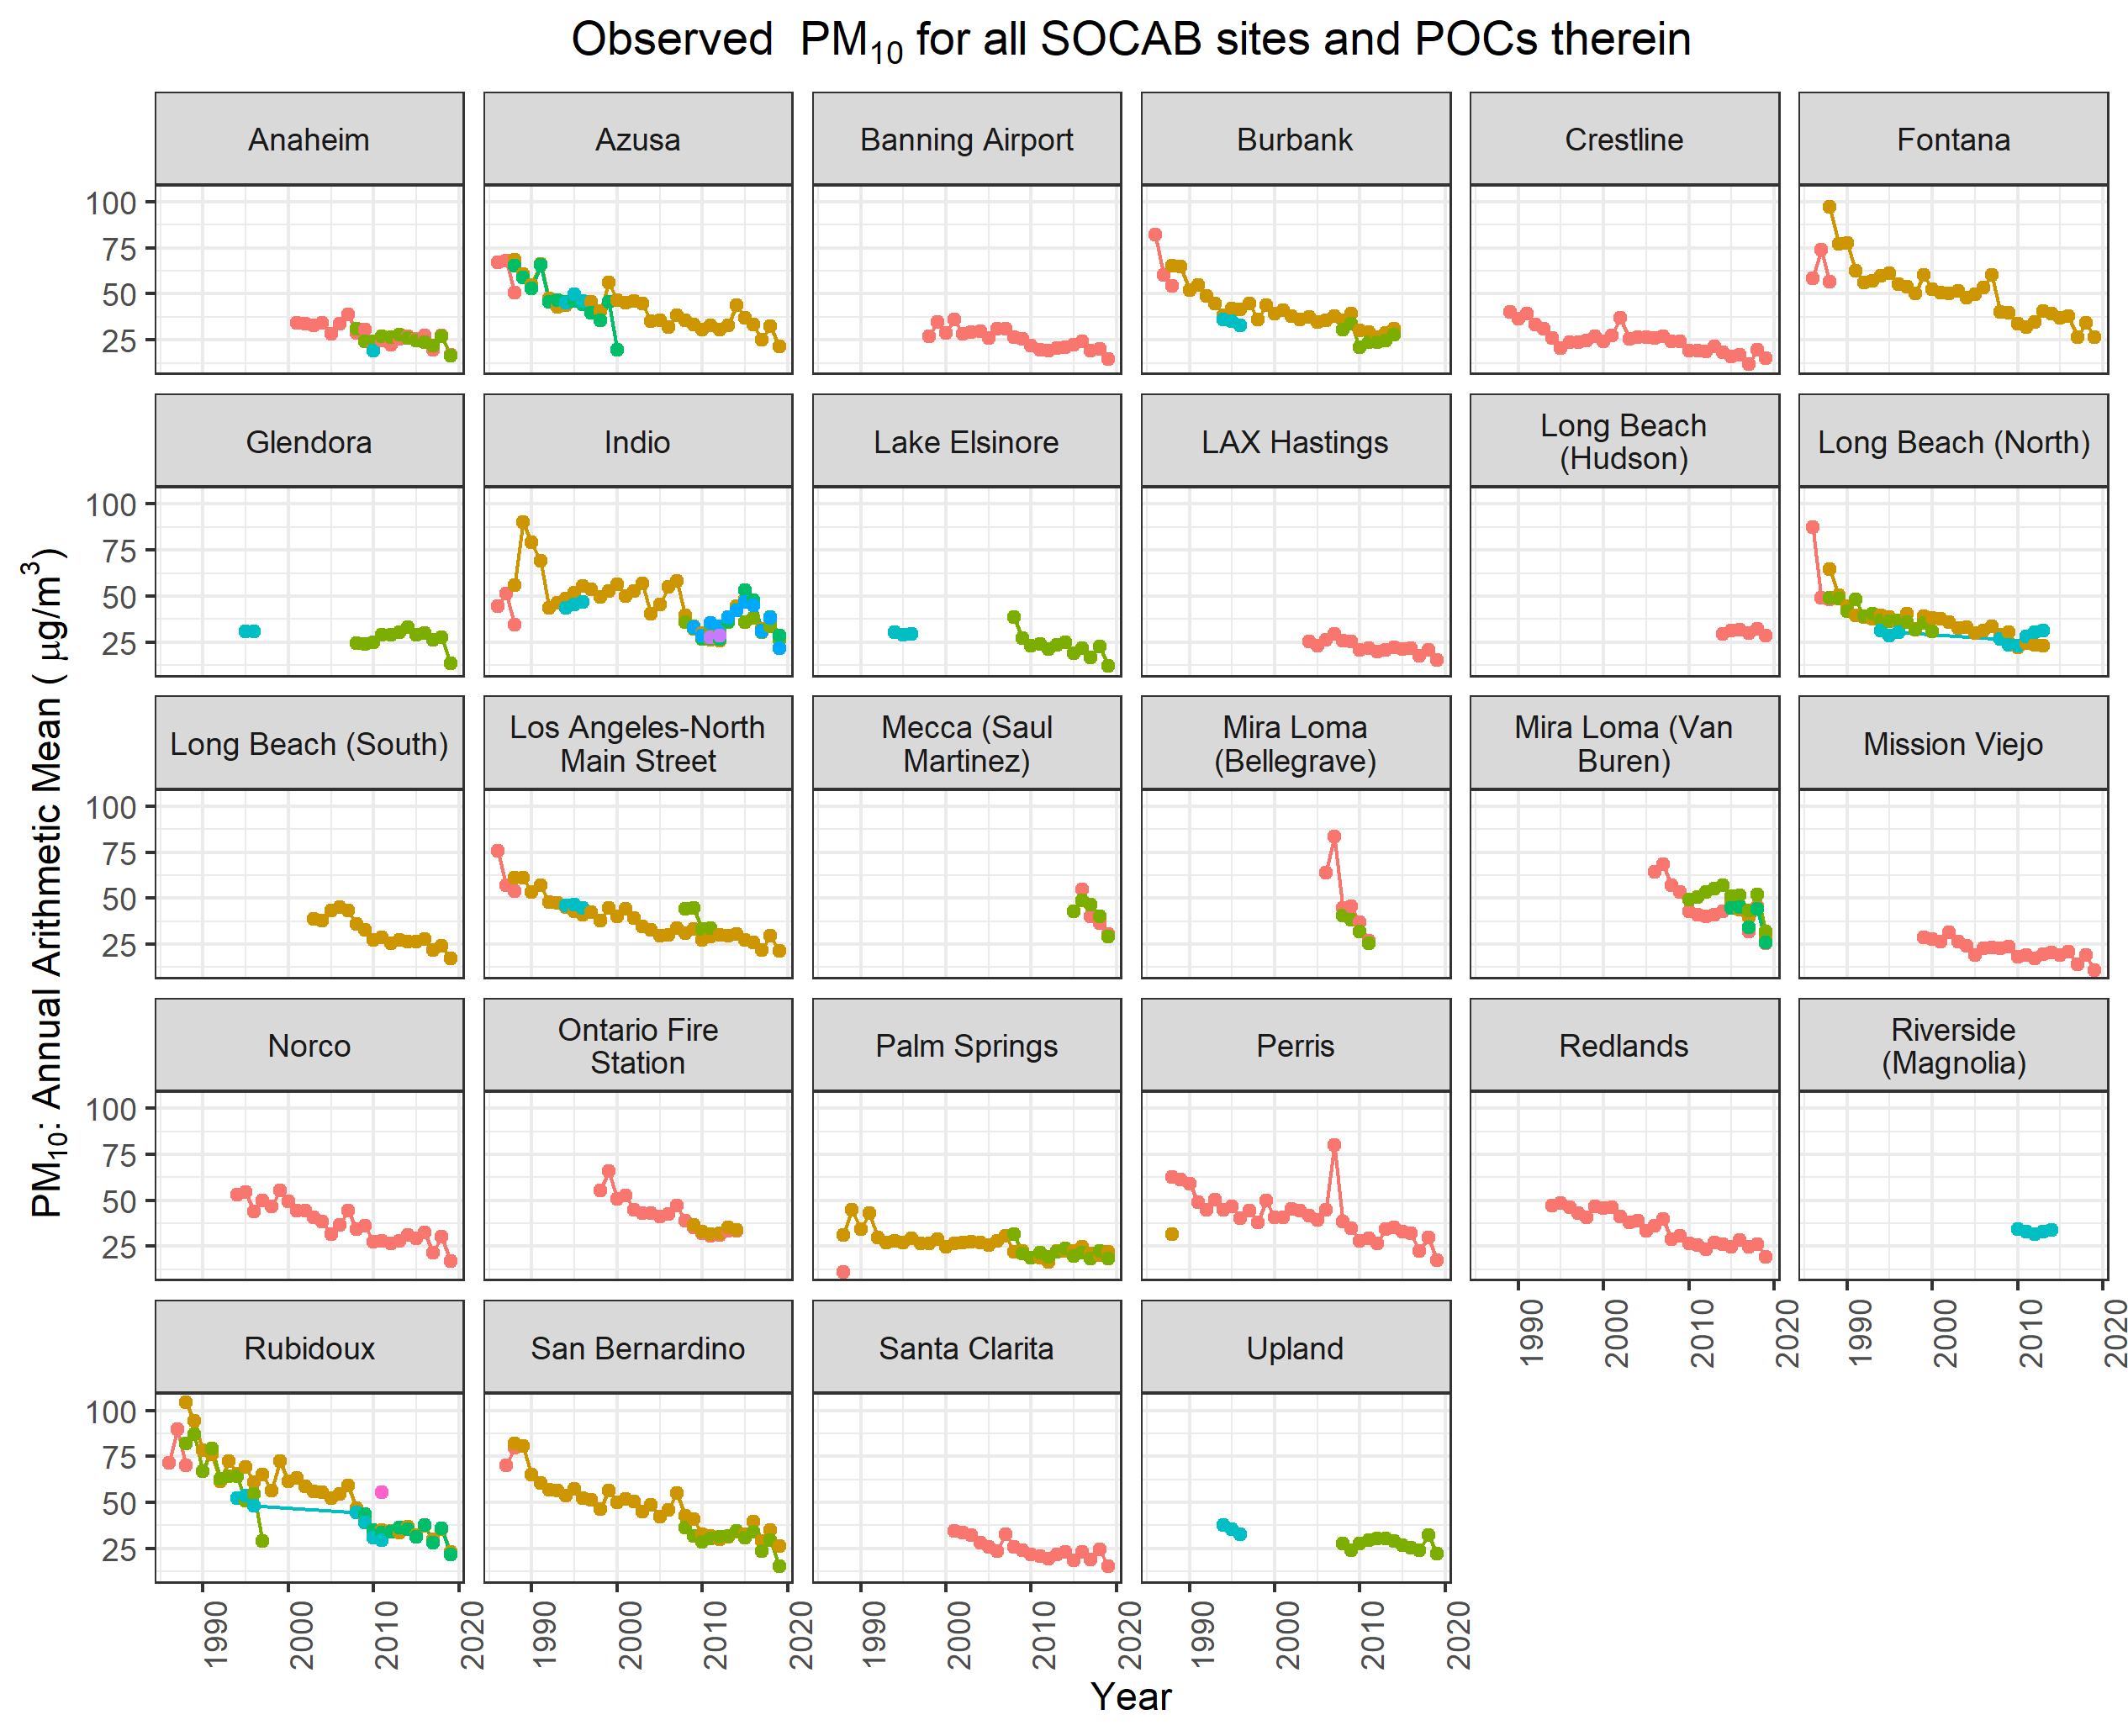
\includegraphics[width = \textwidth]{Figures/POC_all_trace.png}
\caption{Traces showing every sensor (i.e. \ac{POC}) recorded at each site.  Colours are only to distinguish different \ac{POC} and have no meaning between sites.  Notice Azusa, Burbank, Fontana, Indio, Long Beach, Los Angeles-North, Palm Springs, Perris, Rubidoux, and San Bernardino all have a \ac{POC} that stops being used in 1988 (generally coloured red) and is replaced by another \ac{POC} (generally brown) that consistently has a higher concentration of PM10.  Rubidoux and Long Beach (North) both have a \ac{POC} (teal) that was discontinued in 1996 and then reestablished in 2007. These are continuous monitoring \ac{FEM} along with Burbank, Glendora, Indio, Lake Elsinore, Los Angeles - North, and Upland which also have a teal sensor discontinued and eventually replaced by a green sensor.}
\label{fig:POC_all_trace}
\end{figure}

\subsection{Exploratory Data Analysis}
\label{subsec:eda}
Before applying complex INLA modelling to the question of preferential sampling, an exploratory data analysis was carried out.  This analysis provided a sanity check for data acquisition and cleaning, highlighted unusual patterns, and provided preliminary suggestions for preferential sampling.


\subsubsection*{Data Transformation}
\label{subsubsec:datatrans}
\cite{ott1990} suggests that particulate counts follow a log-normal distribution due to the physical processes that make the particulates.  Taking the log of the raw counts helps to stabilize the variance.  This was done by \cite{cameletti2011spatio}  in their similar work examining PM10 concentrations in Italy.

Since log scores are unitless, the raw \ac{PM10} data were normalized to the mean \ac{PM10} in 1986 and the log of that ratio was taken, as described in equation \ref{eq:log_transform}.  In equation \ref{eq:log_transform} $t$ is the year, $s$ is a unique site, $Z$ is the transformed data used for future calculations and modelling, and $PM10_{t,s}$ is the raw data for the year $t$ at site $s$.  Finally, $PM10_{1986,\cdot}$ is the mean of the all observed \ac{PM10} in 1986, 69.65397 $\mu g/m^3$.  This log normalized value of the \ac{PM10} is used for all future analyses.
\begin{equation}
Z_{t,s} = log(PM10_{t,s}/ PM10_{1986,\cdot})
\end{equation} \label{eq:log_transform}


\subsubsection*{Temporal Effects}
\label{subsubsec:tempeffects}
An initial examination of figure \ref{fig:site_trend-ArthmM_NumSites} shows the concentration of \ac{PM10} decreasing over time, as expected from the known history of particulate matter.  This could be modelled as either a fixed or a random effect.  Both options were examined, and the results are described in this report.  In this preliminary investigation, all spatial correlations
were ignored.

After preliminary modelling, our focus is on describing preferential sampling, not the decrease in \ac{PM10} over time. Modelling the small perturbations with a Random Walk seemed likely to give a better understanding of what the sites are doing and so a better picture of any possible preferential sampling.  

\subsubsection*{Fixed Temporal effects}
\label{subsubsec:fixedtempeffects}
The first way to model the temporal trend is with a linear model.   While the general trend in means of figure \ref{fig:site_trend-ArthmM_NumSites} appears mostly 1st order to the eye, \cite{shaddick2014case} used a quadratic function to model the decreasing temporal trend in black smoke in the UK. That led us to  investigate both first- and second-order models for the trend over time using equations \ref{eq:linearTime} and \ref{eq:quadraticTime} respectively:
\begin{subequations}
\begin{align}
	Z_{t,\cdot} &= \beta_0 + \beta_1t + \epsilon \label{eq:linearTime} \\ 
	Z_{t,\cdot} &= \beta_0 + \beta_1t + \beta_2t^2 + \epsilon \label{eq:quadraticTime}.
\end{align}
\end{subequations}

Figures  \ref{fig:explore_ts_exp_fit} and \ref{fig:explore_ts_exp_quad_fit} show the results of first and second-order models being fitted to the log normalized \ac{PM10} data.   An \ac{ANOVA} comparing the two models ($anova(model.lm.log, model.lm.log.quad)$) suggests a small but significant improvement of the second order model ($Pr(>F) = 0.0492$) compared to the 1st order. 

Both models do a good job of whitening the overall residual of the annual mean, as seen in the \ac{ACF} and \ac{PACF} plots.   This suggests there might not be an autocorrelation AR(1) process, unlike the model used by \cite{cameletti2011spatio}.

\begin{figure}[ht]
\centering
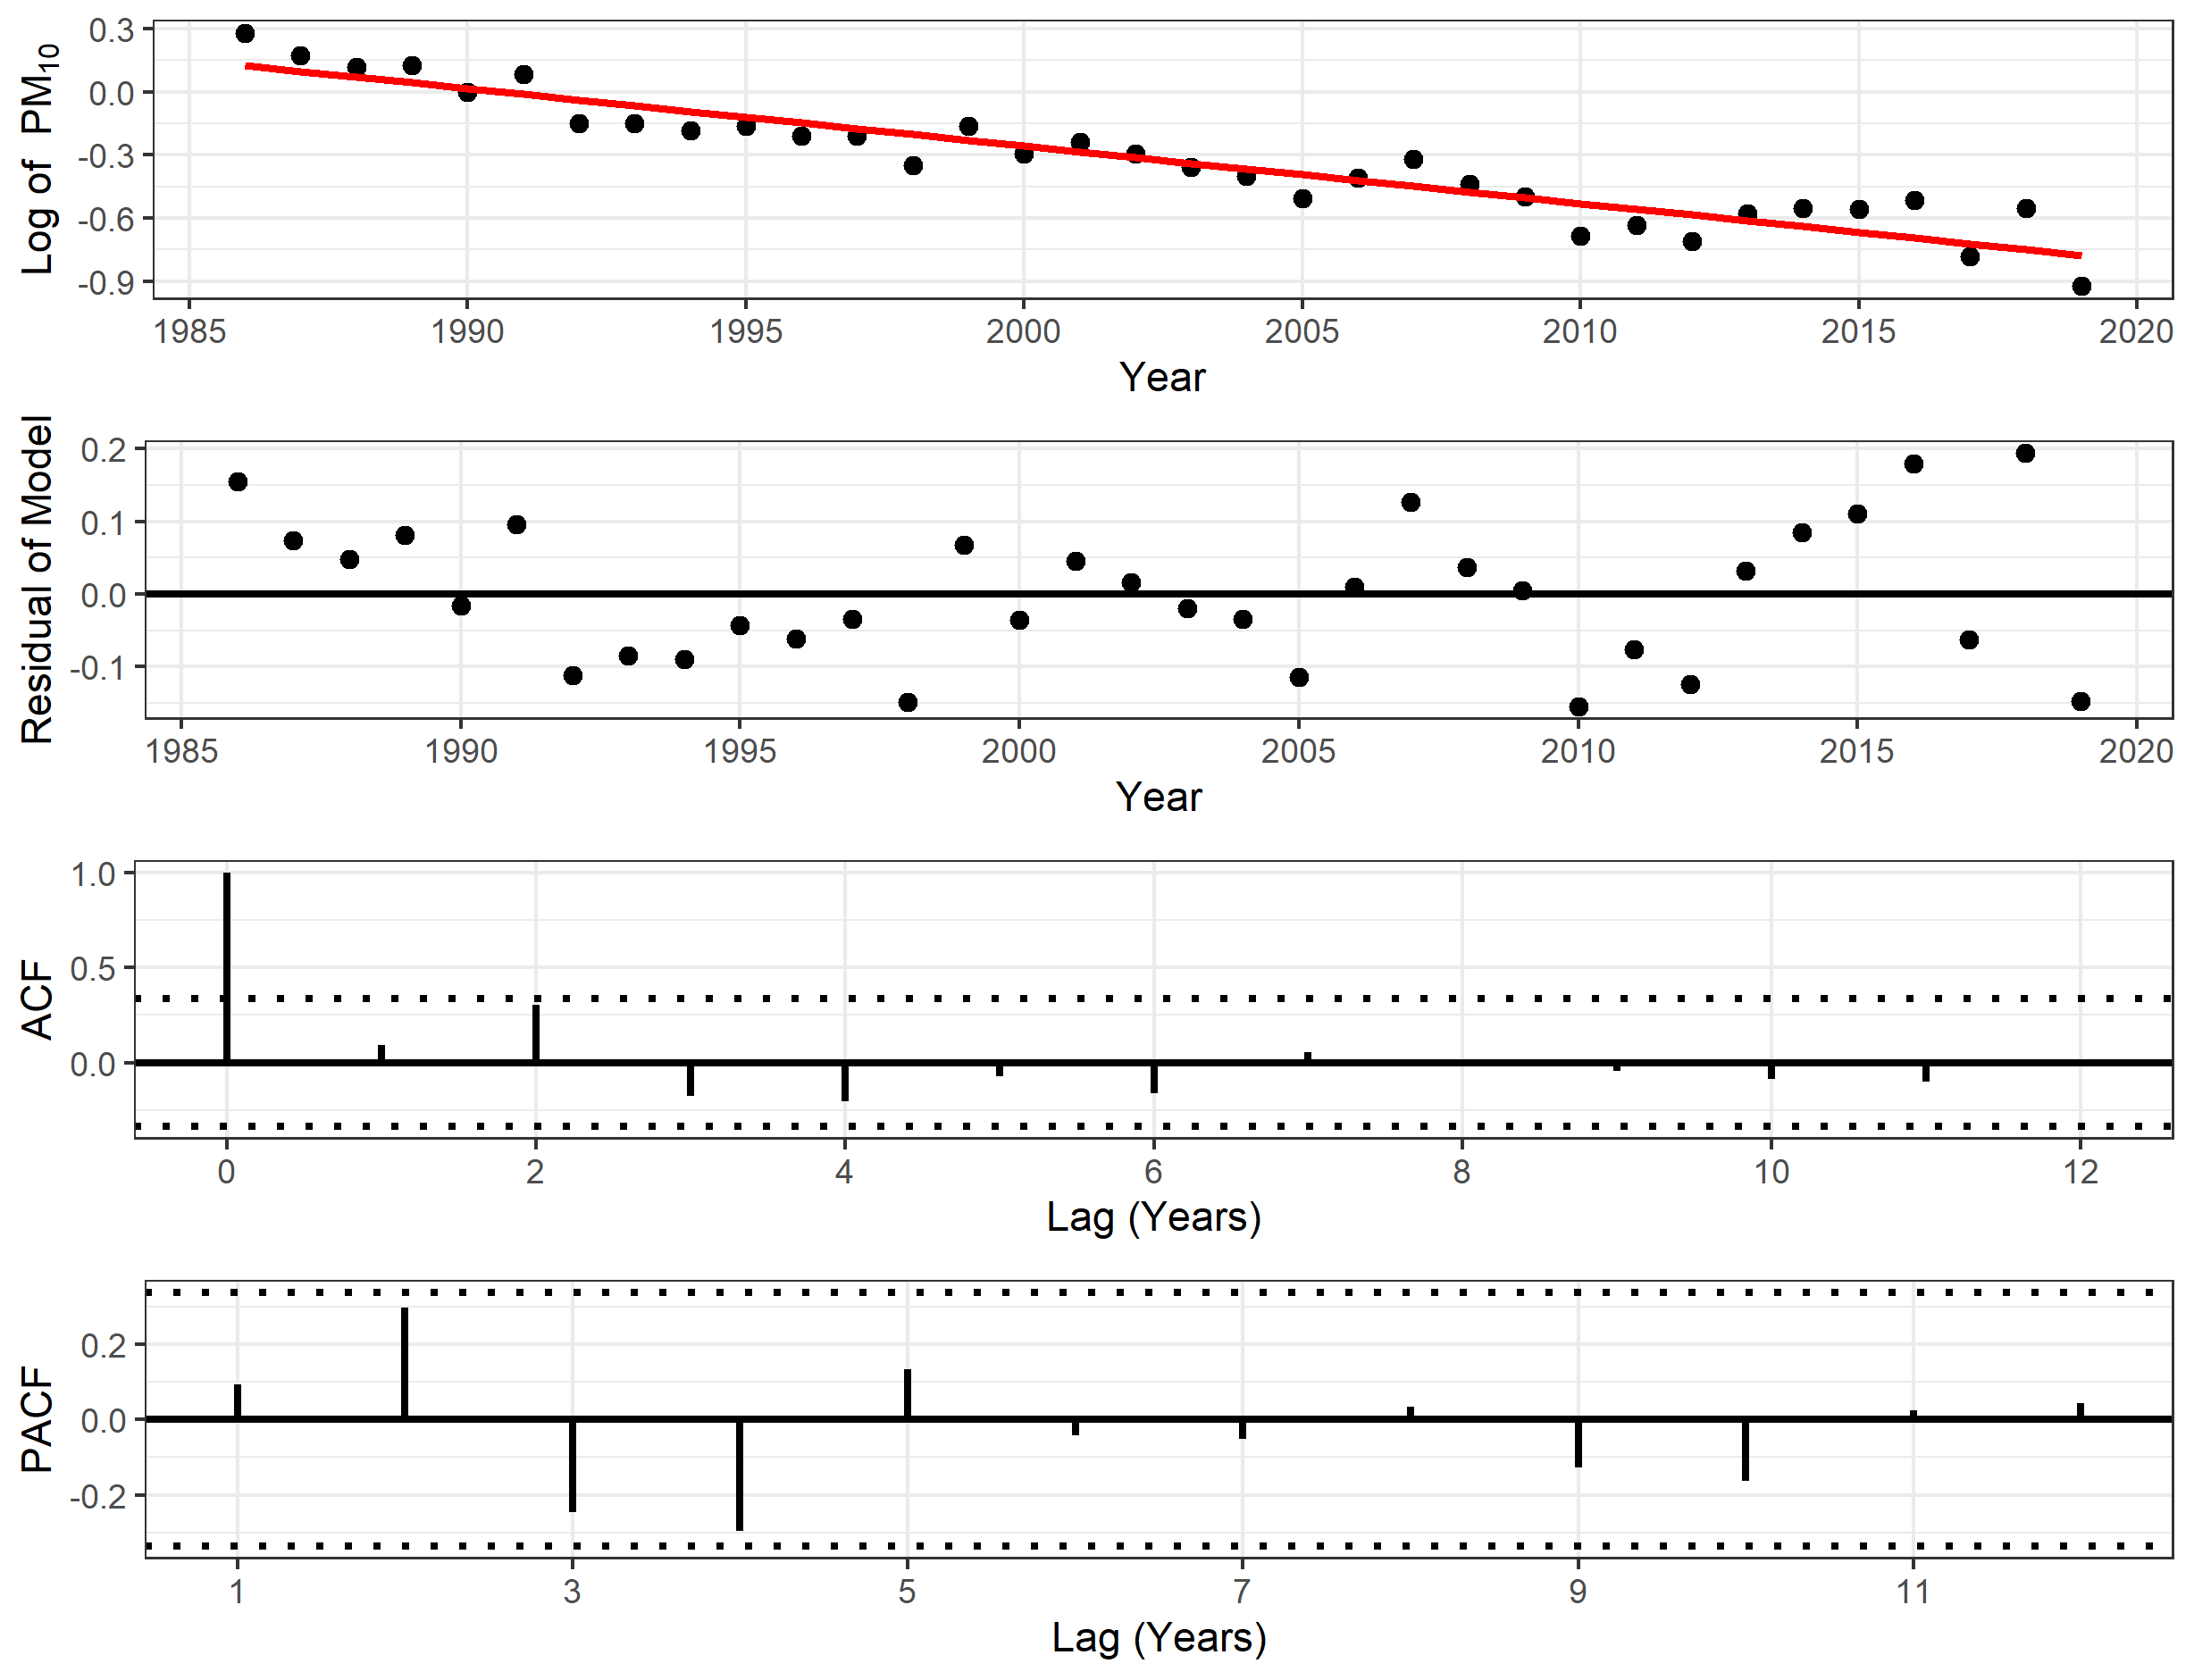
\includegraphics[width = \textwidth]{Figures/explore_ts_exp_fit.png}
\caption{Results of a linear fit to a log transformation of the PM10 data.  The line is the model $Z_{t,s} \sim Year$, and has a slope of -0.027 and adjusted $R^2$ of 0.88.  The \ac{ACF} and \ac{PACF} suggest that the process remaining is probably white noise.  Dots are the Median of the arithmetic mean of each year.  The dotted line shows a confidence limit of $qnorm((1 + ci)/2)/sqrt(n)$, R's default for ACF and PACF.  This stems from Chatfield's Analysis of Time Series (1980), in which he describes how the variance of the autocorrelation coefficient at lag k, is normally distributed at the limit, and that $Var(rk) \sim 1/N$ (where N is the number of observations).}
\label{fig:explore_ts_exp_fit}
\end{figure}

\begin{figure}[ht]
\centering
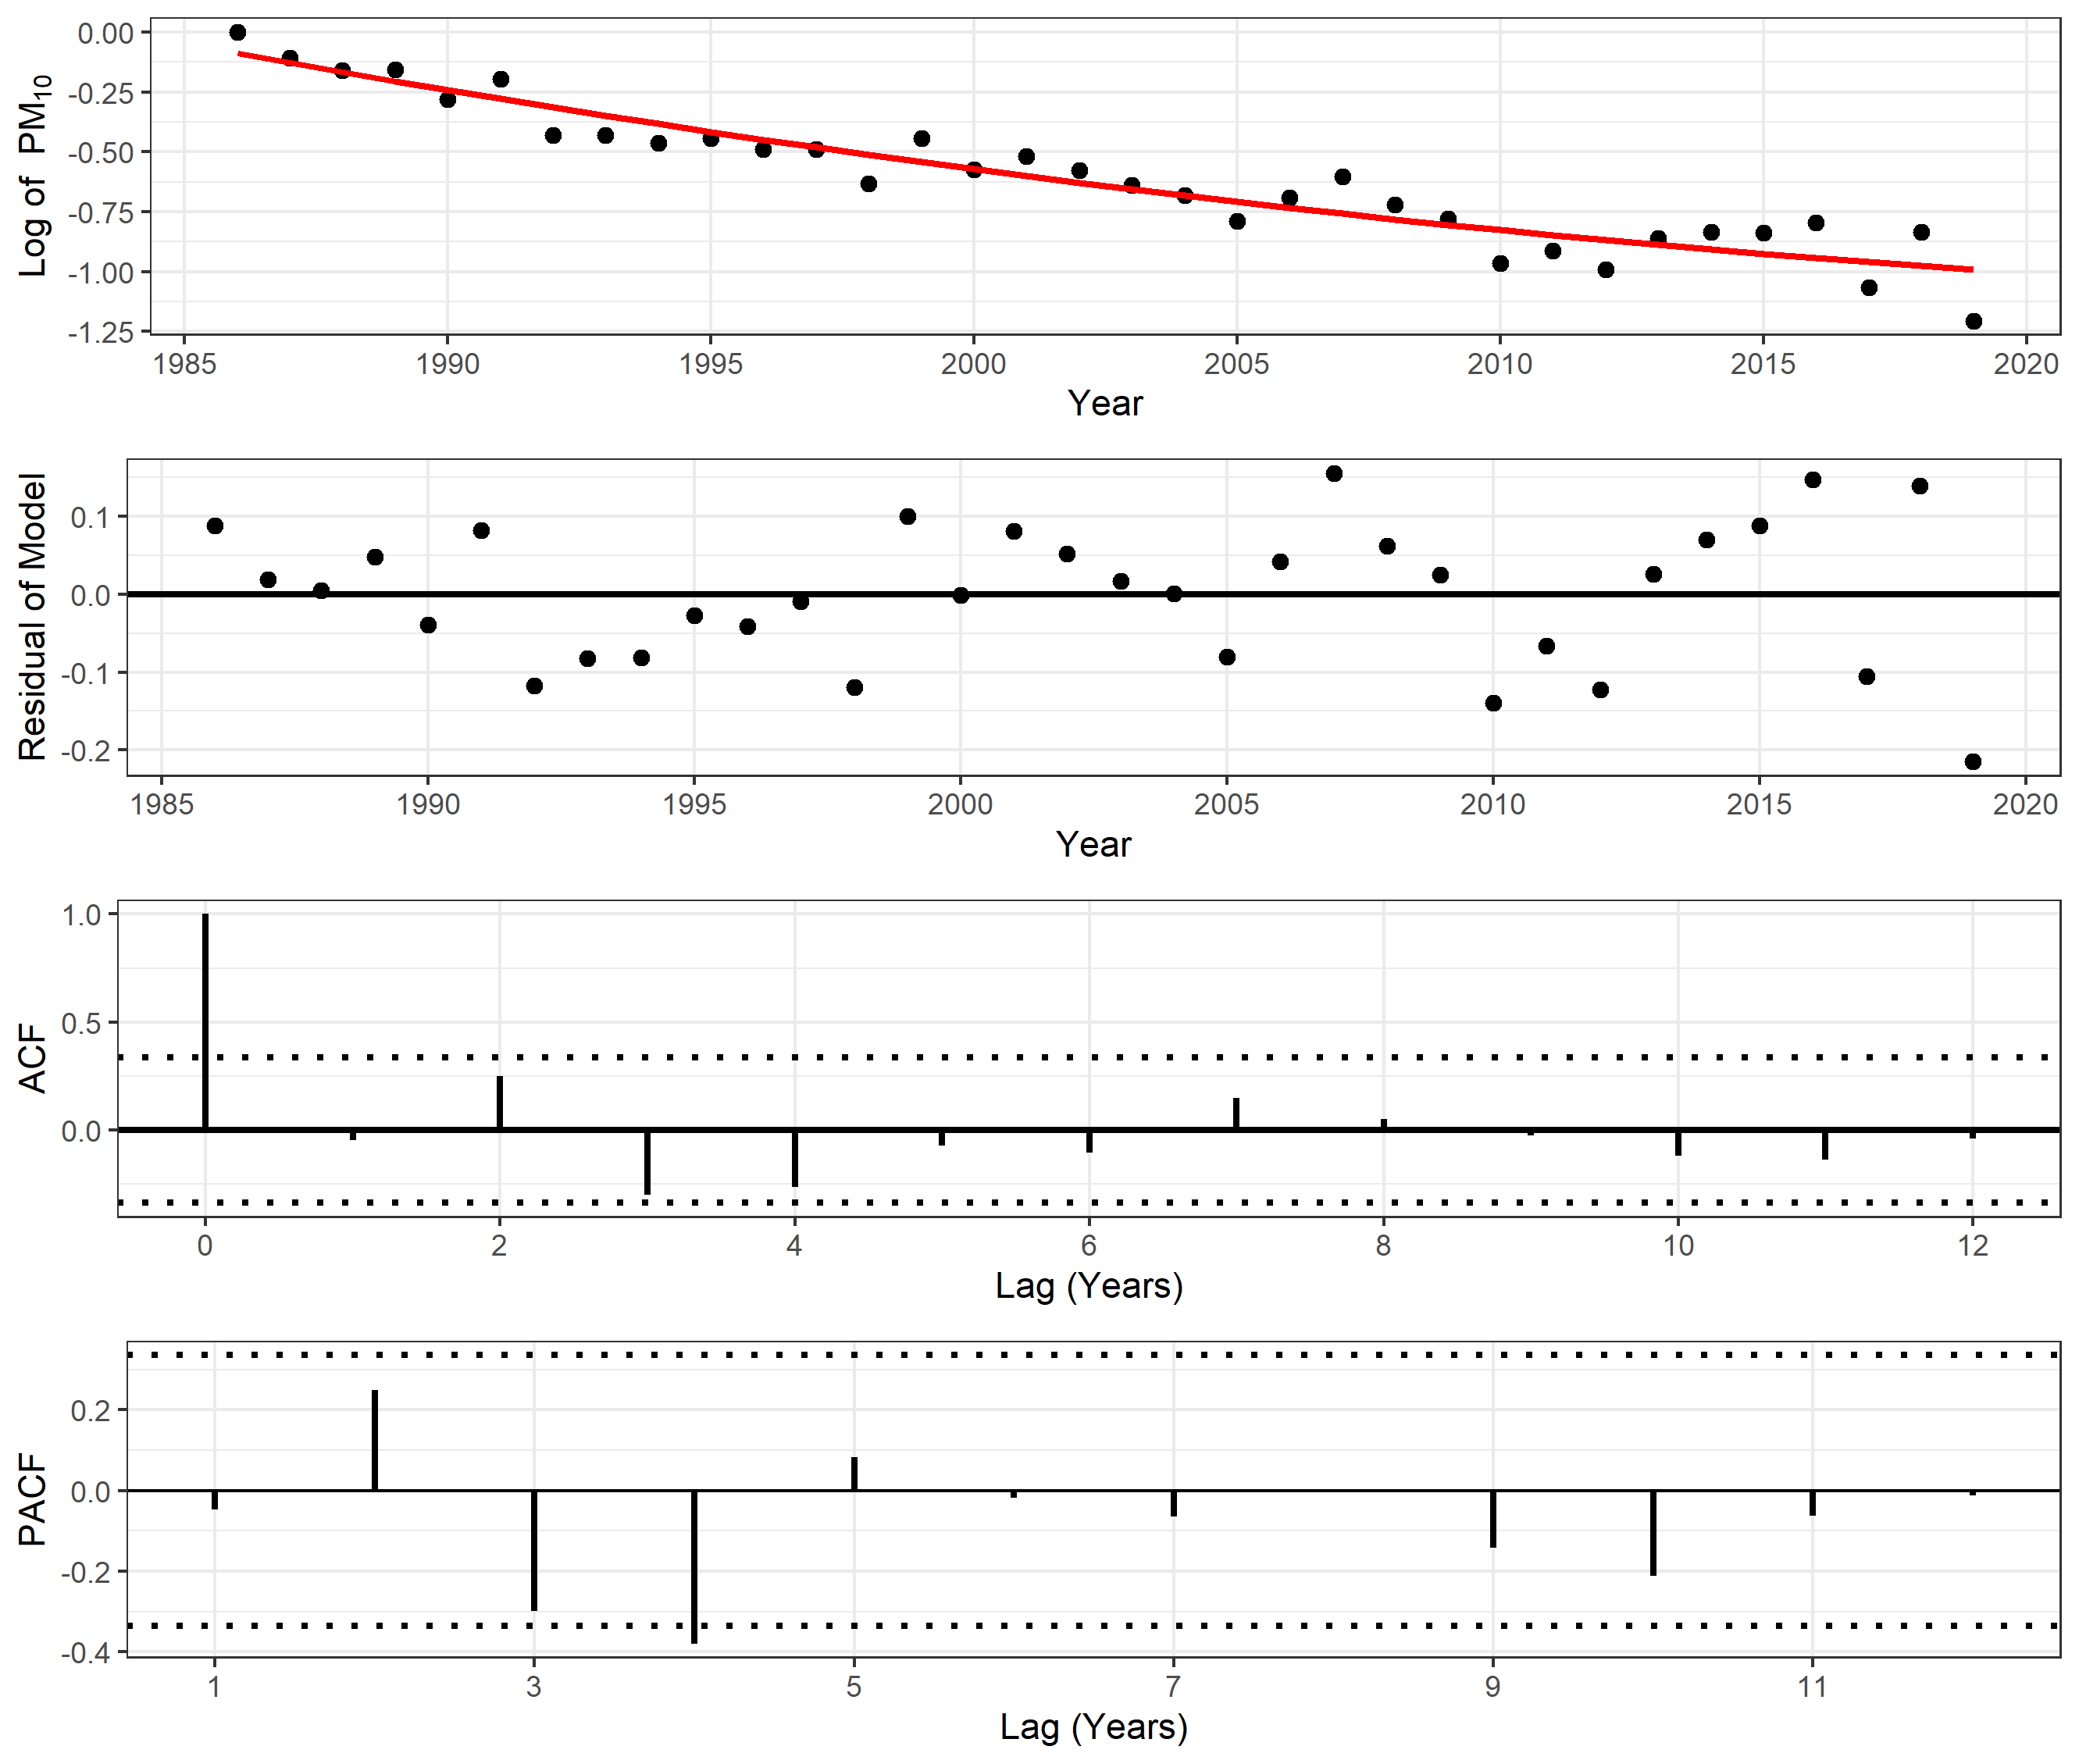
\includegraphics[width = \textwidth]{Figures/explore_ts_exp_quad_fit.png}
\caption{Results of a linear fit to the PM10 data.  The line is the model $Z_{t,s} \sim \beta_1 Year+ \beta_2 Year^2$ and has coefficients $\beta_1 = -1.56$ and $\beta_2 = 0.00038$ and adjusted $R^2$ of  0.90.  The \ac{ACF} and \ac{PACF} plots of the residuals suggest there might be an MA(1) or AR(1) process.  Dots are the Median of the arithmetic mean of each year. The dotted line shows a confidence limit of $qnorm((1 + ci)/2)/sqrt(n)$, R's default for plots of ACF and PACF. }
\label{fig:explore_ts_exp_quad_fit}
\end{figure}

\subsubsection*{Temporal Trend as a Random Walk} \label{subsubsec:RWexploration}
An alternative approach to accounting for a broad-scale trend in time is to use a random variable.  The logic supporting the use of a random variable over a fixed effect lies in our lack of interest in estimating the annual decrease, and a model that can be more adaptive to yearly fluctuations can fit closer and give a better understanding of the field at the time.  Two options are a random walk and a 1-dimensional Mat\'{e}rn interpolation with \ac{INLA}.  Because the random walk is simpler, that was chosen.

\begin{figure}[ht]
\centering
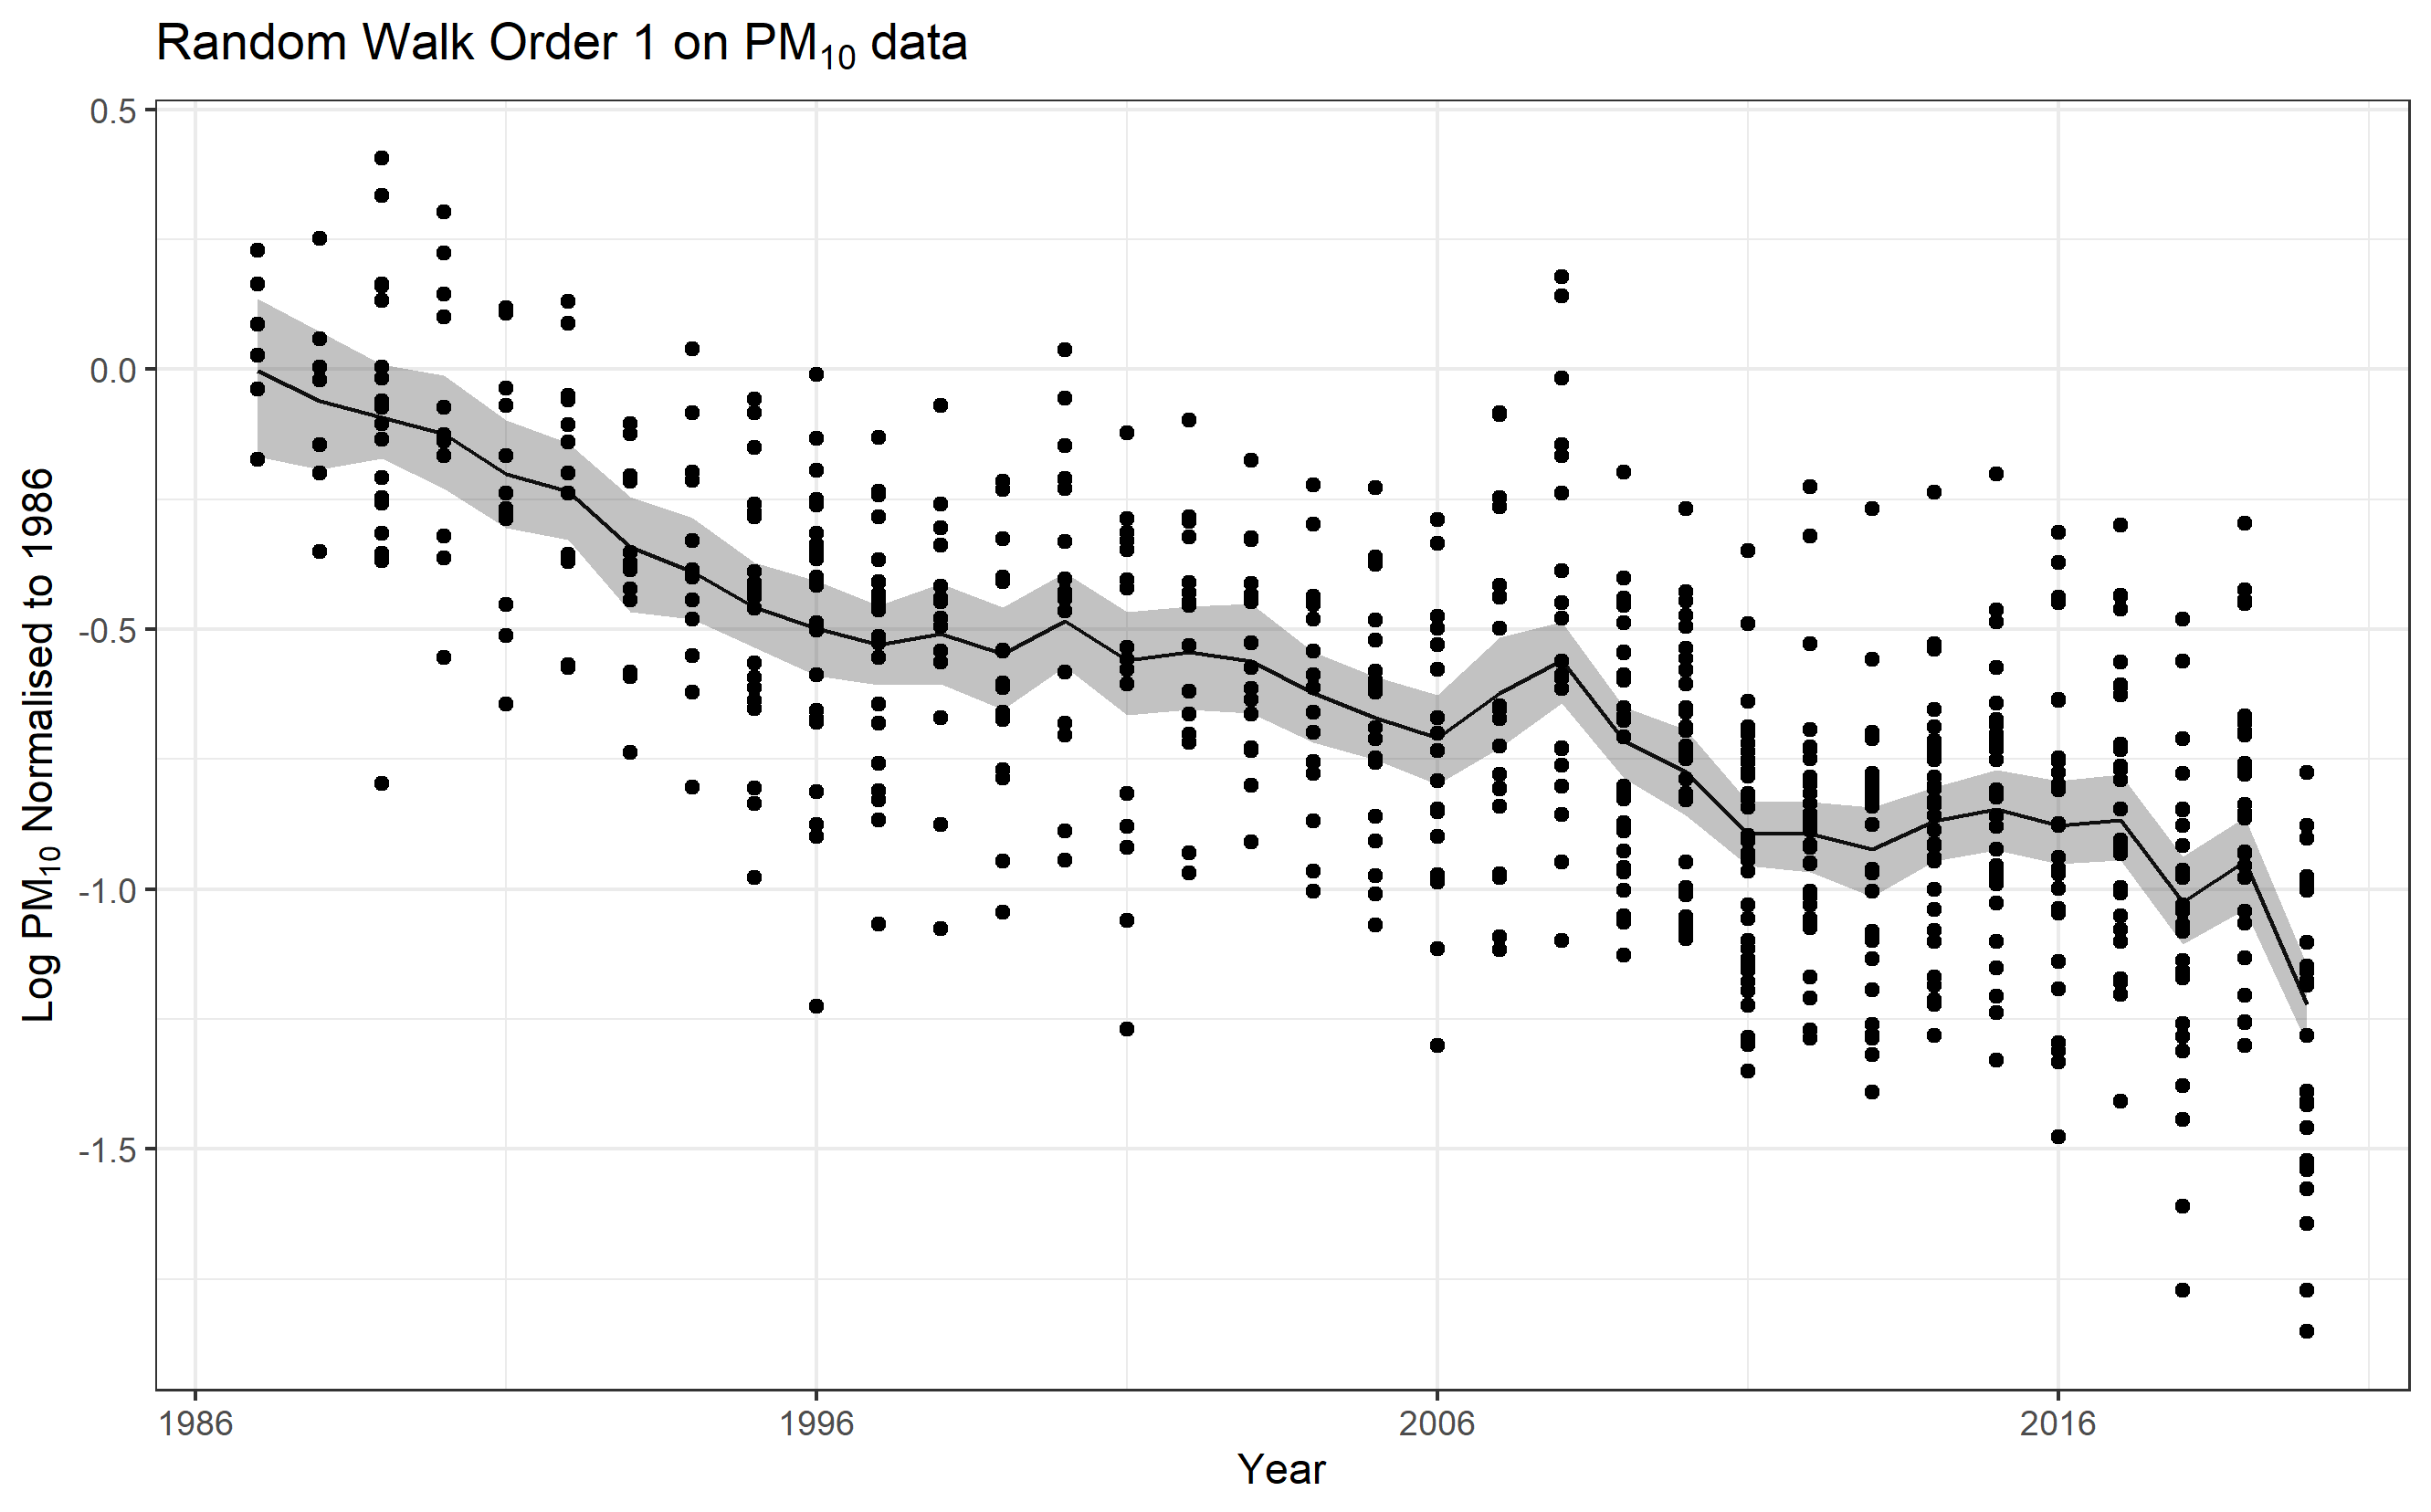
\includegraphics[width = \textwidth]{Figures/Random_Walk1.png}
\caption{First order Random Walk smoothing sets a prior on the difference between each observed value $f(\kappa_i)$.  Like so: $f(\kappa_{i+1}) - f(\kappa_i) \Tilde{} N(0,\tau)$ }
\label{fig:Random_Walk1}
\end{figure}

\begin{figure}[ht]
\centering
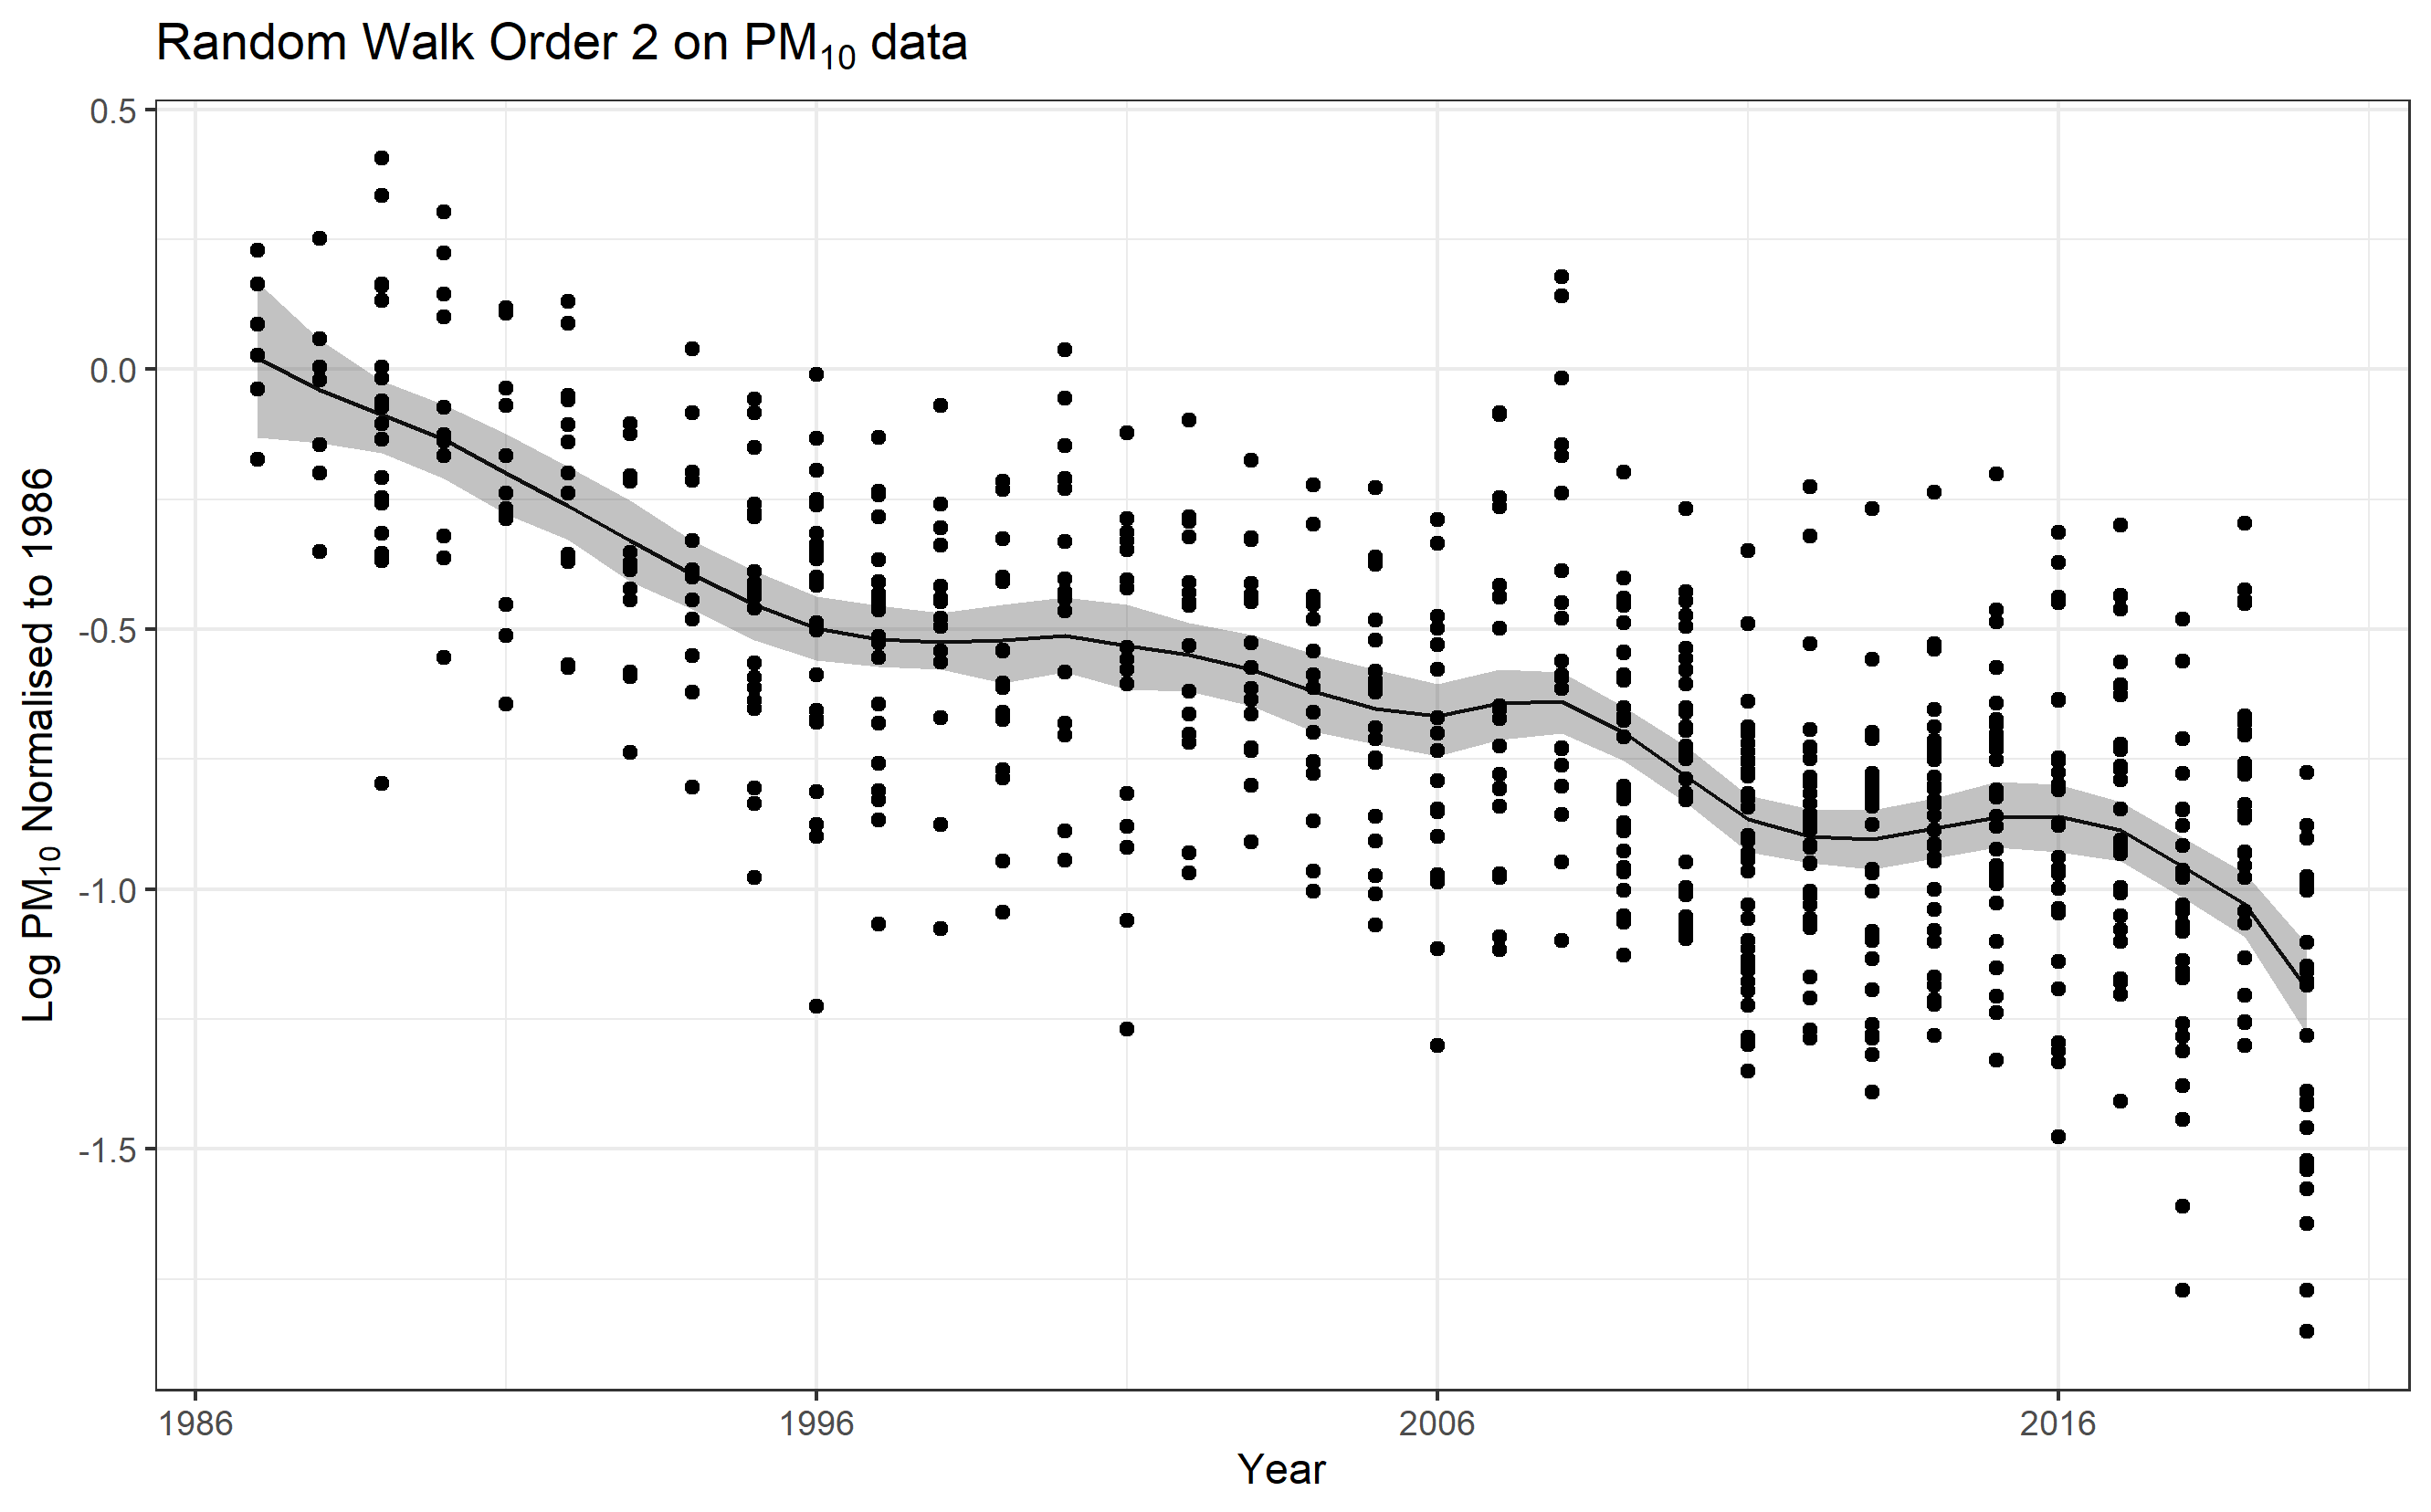
\includegraphics[width = \textwidth]{Figures/Random_Walk2.png}
\caption{Second order Random Walk smoothing sets a prior on the difference between each observed value $f(\kappa_i)$.  Like so:  $f(\kappa_{i+1}) - 2f(\kappa_i) + f(\kappa_{i-1}) \sim N(0, \tau)$}
\label{fig:Random_Walk2}
\end{figure}

First-order smoothing, shown in Figure \ref{fig:Random_Walk1}, looks spiky, and second-order smoothing, \ref{fig:Random_Walk2} seems better. Table \ref{tab:RW_parameters} describes the results of the two orders of smoothing, and the DIC criterion suggests that the 1st order smoothing is marginally better than the 2nd order smoothing.

As discussed in the section on priors, section \ref{subsubsec:Priors}, the \ac{PC} prior for the precision of the RW is set as the empirical SD of the data, which is $0.3729848$ when not accounting for the structure of sites and \ac{POC}s.
\begin{lstlisting}[language=R]
pc_prior <-list(theta =list(prior =``pc.prec'',
param =c(data.emp.sd,0.01)))
\end{lstlisting}

\begin{table}[ht]
\centering
\begin{tabular}{p{0.25\linewidth}|p{0.30\linewidth}|p{0.30\linewidth}}
	Parameter & RW 1 &  2 \\ \hline
	Model WAIC & 1.187e+02 & 1.285e+02\\
	Model DIC & 1.187e+02 & 1.283e+02 \\
	\hline
	Intercept Mean & 3.407793e-05 & 2.074067e-05 \\
	Intercept SD & 31.62663 & 31.69167 \\
	\hline
	RW trend range, mean: & [-1.2189, -0.00401586] & [-1.19403, 0.0299855] \\
	RW trend sd, range: & [31.6266, 31.6267] & [31.6917, 31.6918] \\
	\hline
	Hyperpar: Precision of Gaussian observation Mean & 14.9708 & 14.38641 \\
	Hyperpar: Precision of Gaussian observation SD & 0.8224243 & 0.5420988 \\
	Hyperpar: Precision of Random Walk Parameter Mean & 106.8693 & 814.72112 \\
	Hyperpar: Precision of Random Walk Parameter SD & 41.5575799 & 961.1867062 \\
	
\end{tabular}
\caption{Comparison between exploratory models for a \ac{RW}1 and \ac{RW}2 model for the trend over years.  Neither model has a spatial component, and they treat sites and \ac{POC}s in the same year as \ac{IID} instead of nesting them in any way: y = intercept + RW. }
\label{tab:RW_parameters}
\end{table}

The R package \lstinline{inlabru} generates a Random walk of order one on the time series using the following code:
\begin{lstlisting}[language = R]
cmp.spline1.PM10 <- log.Arthmt.M ~ Intercept + trend(map = yeari,
model = ``rw1'',
constr = FALSE,
n = n_year,
hyper = pc_prior)
bru.spline1.PM10 <- bru(cmp.spline1.PM10,
family = ``gaussian'',
data = test)

\end{lstlisting}

Similarly, a second-order random walk in R was generated as follows:
\begin{lstlisting}[language = R]
cmp.spline2.PM10 <- log.Arthmt.M ~ Intercept + trend(map = yeari,
model = ``rw2'',
constr = FALSE,
n = n_year,
hyper = pc_prior)
bru.spline2.PM10 <- bru(cmp.spline2.PM10,
family = ``gaussian'',
data = test)

\end{lstlisting}

\subsubsection{Metadata}
\label{subsubsec:metadata}
Finally, gross patterns in the mean could exist and be described by the metadata available and included in a final model as fixed effects.  Here is a brief discussion of the categorical metadata variables available from the \ac{SCAQMD} and the \ac{EPA} that were examined as possible inclusions.

The three variables, which were examined,  were Land Use (e.g. commercial, residential, industrial, agricultural), Land Density (e.g. urban, rural, suburban), and Site Classification (e.g. background, high concentration, population exposure).

A quick examination of the Land Use and Land Density, (both from the \ac{EPA}'s metadata) in Figures \ref{fig:SOCAB_metadata_Site_Land_use} and \ref{fig:SOCAB_metadata_Site_Status} respectively, show that these categories will have little help in making predictions.

The \ac{SCAQMD} provides the Site Classification.  These categories seem to have different means from each other, see Figure \ref{fig:SOCAB_metadata_Site_Type}, but only in that sites designed to capture high concentration do so.  Since the effort is to describe preferential sampling and not relations to covariates, this tautology seems unhelpful for modelling the \ac{PM10} field.  Future work that tries to model site inclusion or removal might find the Site Classification useful.  

\begin{figure}[ht]
\centering
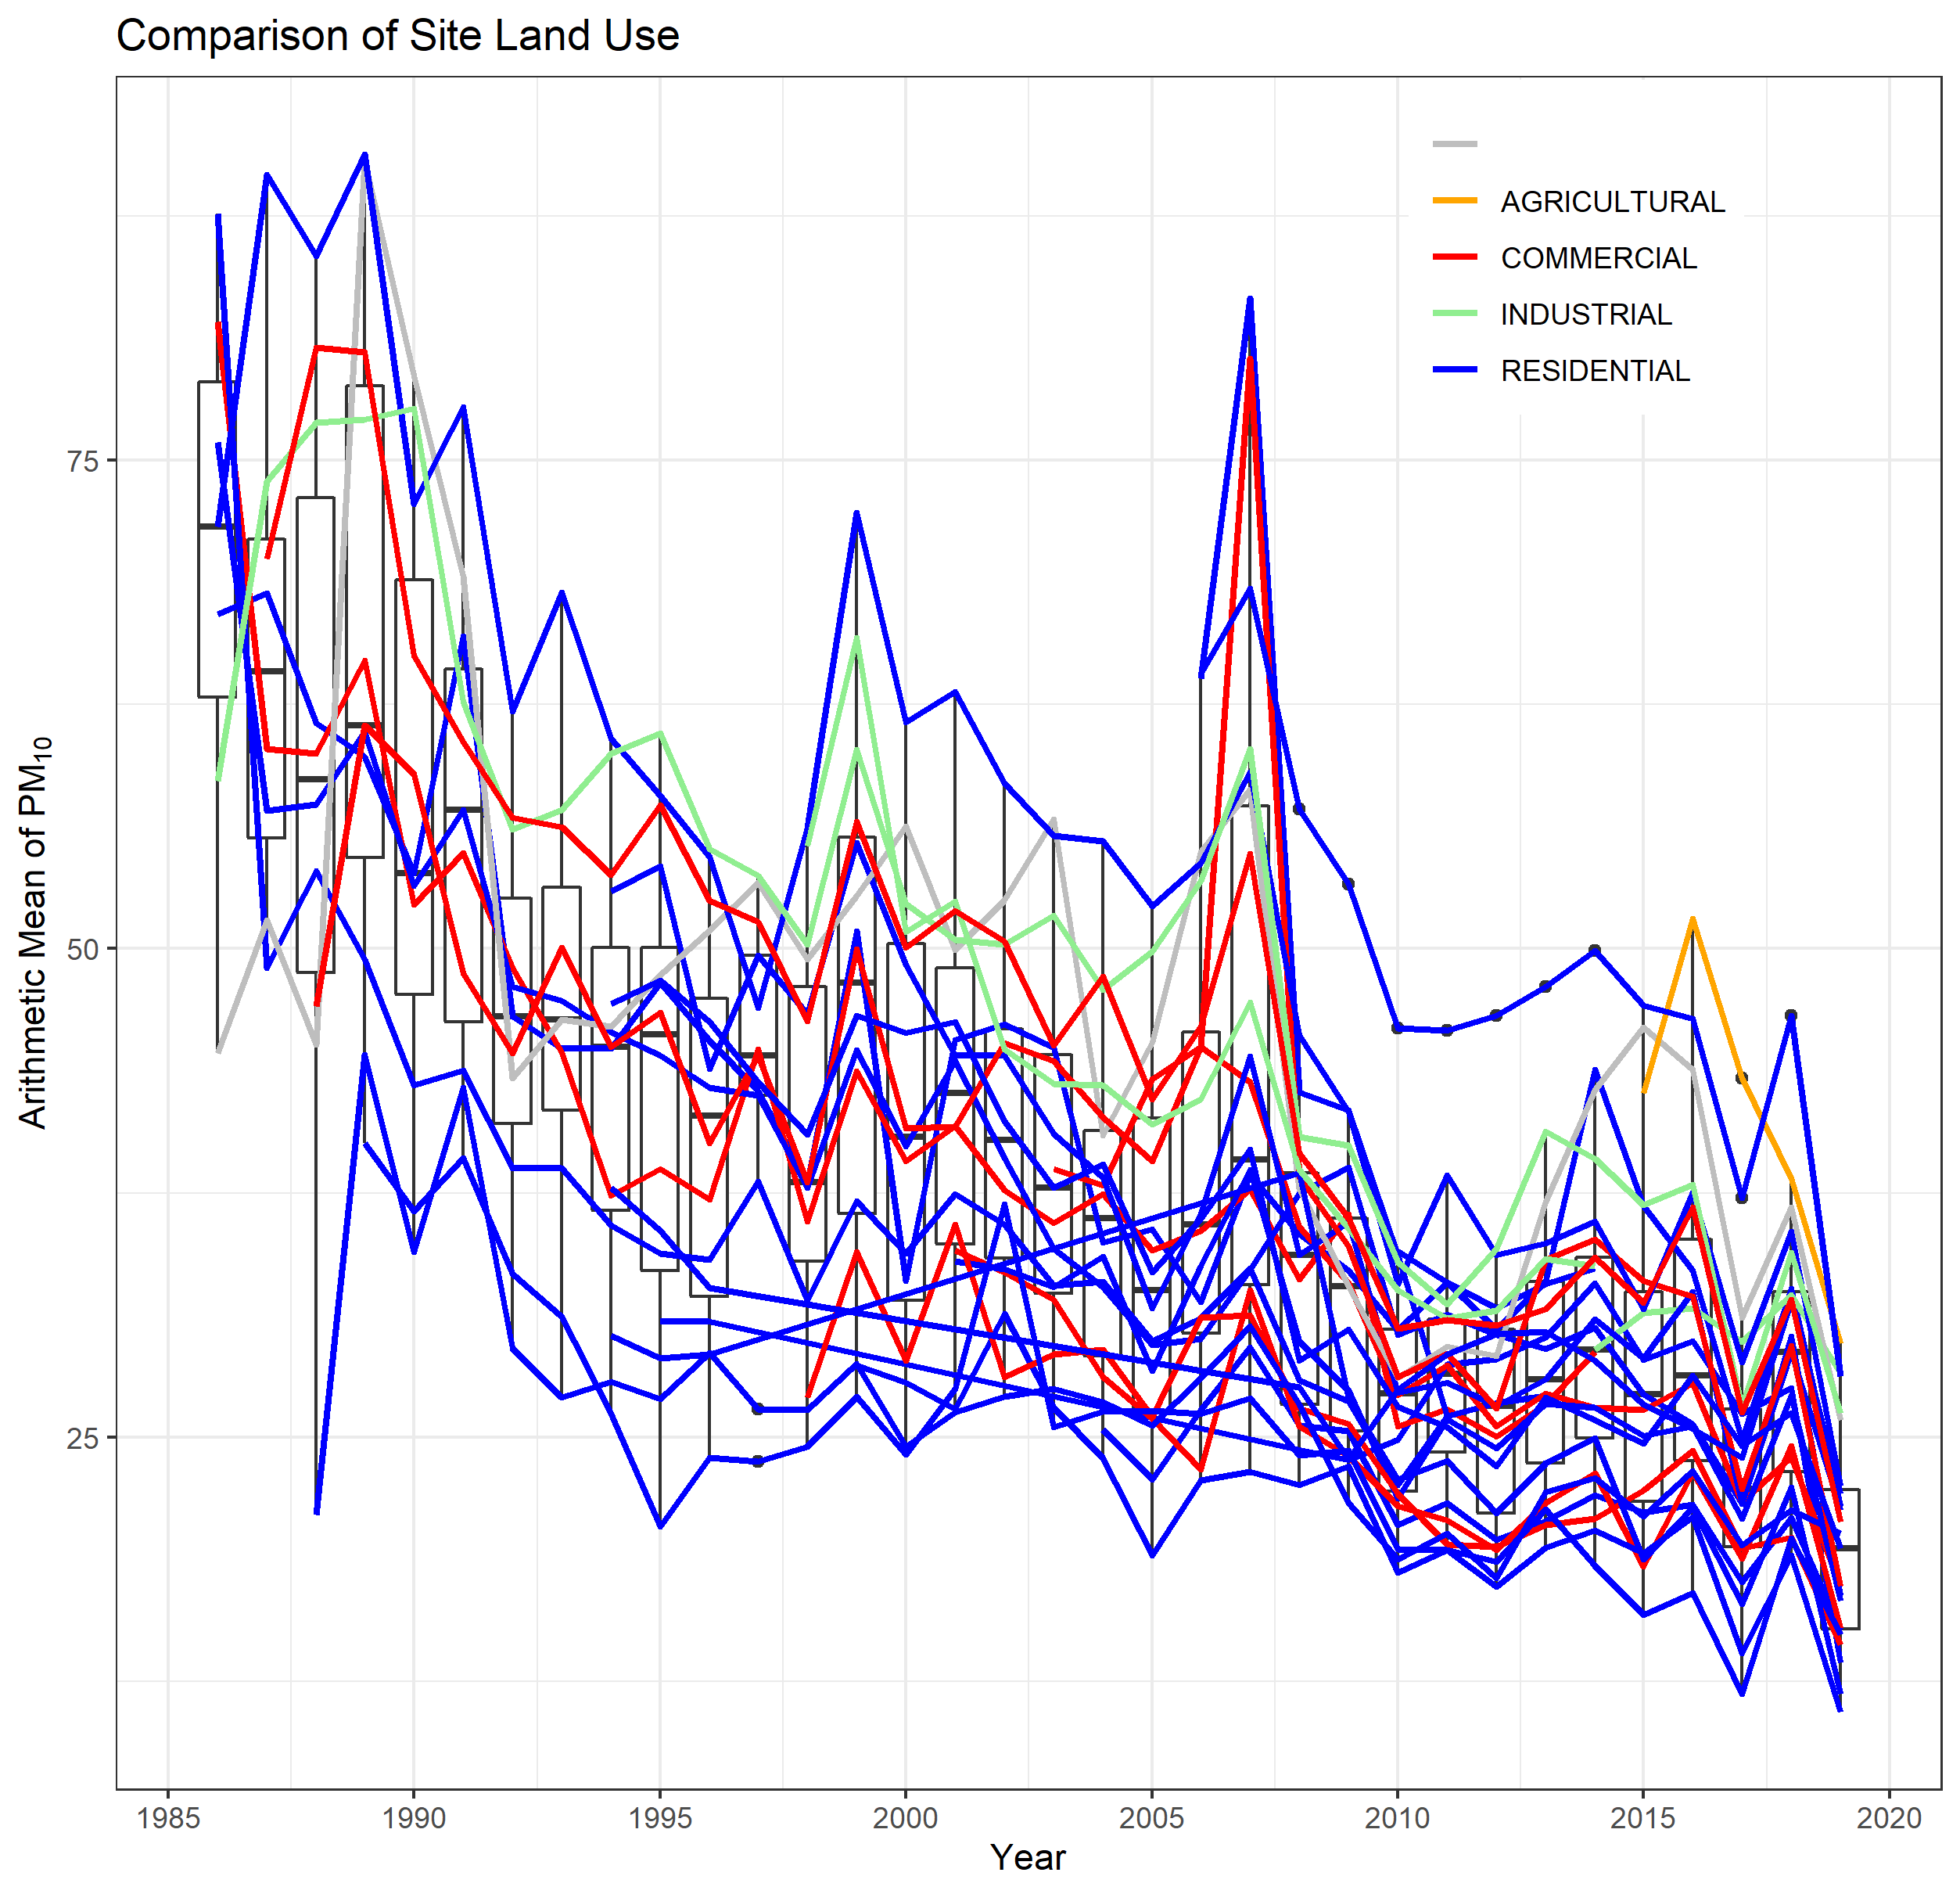
\includegraphics[width = \textwidth]{Figures/SOCAB_metadata_Site_Land_use.png}
\caption{This shows the site traces coloured by the type of human activity being carried out in the vicinity of each site as defined by the EPA.  In the case of multiple \ac{POC}s in at one site, the mean of those \ac{POC}s is taken.  One site was given no category and is in Grey.  The vast majority of sites are either Commercial (red, 6 sites total) or Residential (blue, 17 sites total) and these two categories are mixed relatively homogeneously.  Industrial (light green, 3 sites total) and Agricultural (Orange, 1 site) sites stand out as generally being elevated above the IQR for each year's observations, but have a handful of total sites.}
\label{fig:SOCAB_metadata_Site_Land_use}
\end{figure}

\begin{figure}[ht]
\centering
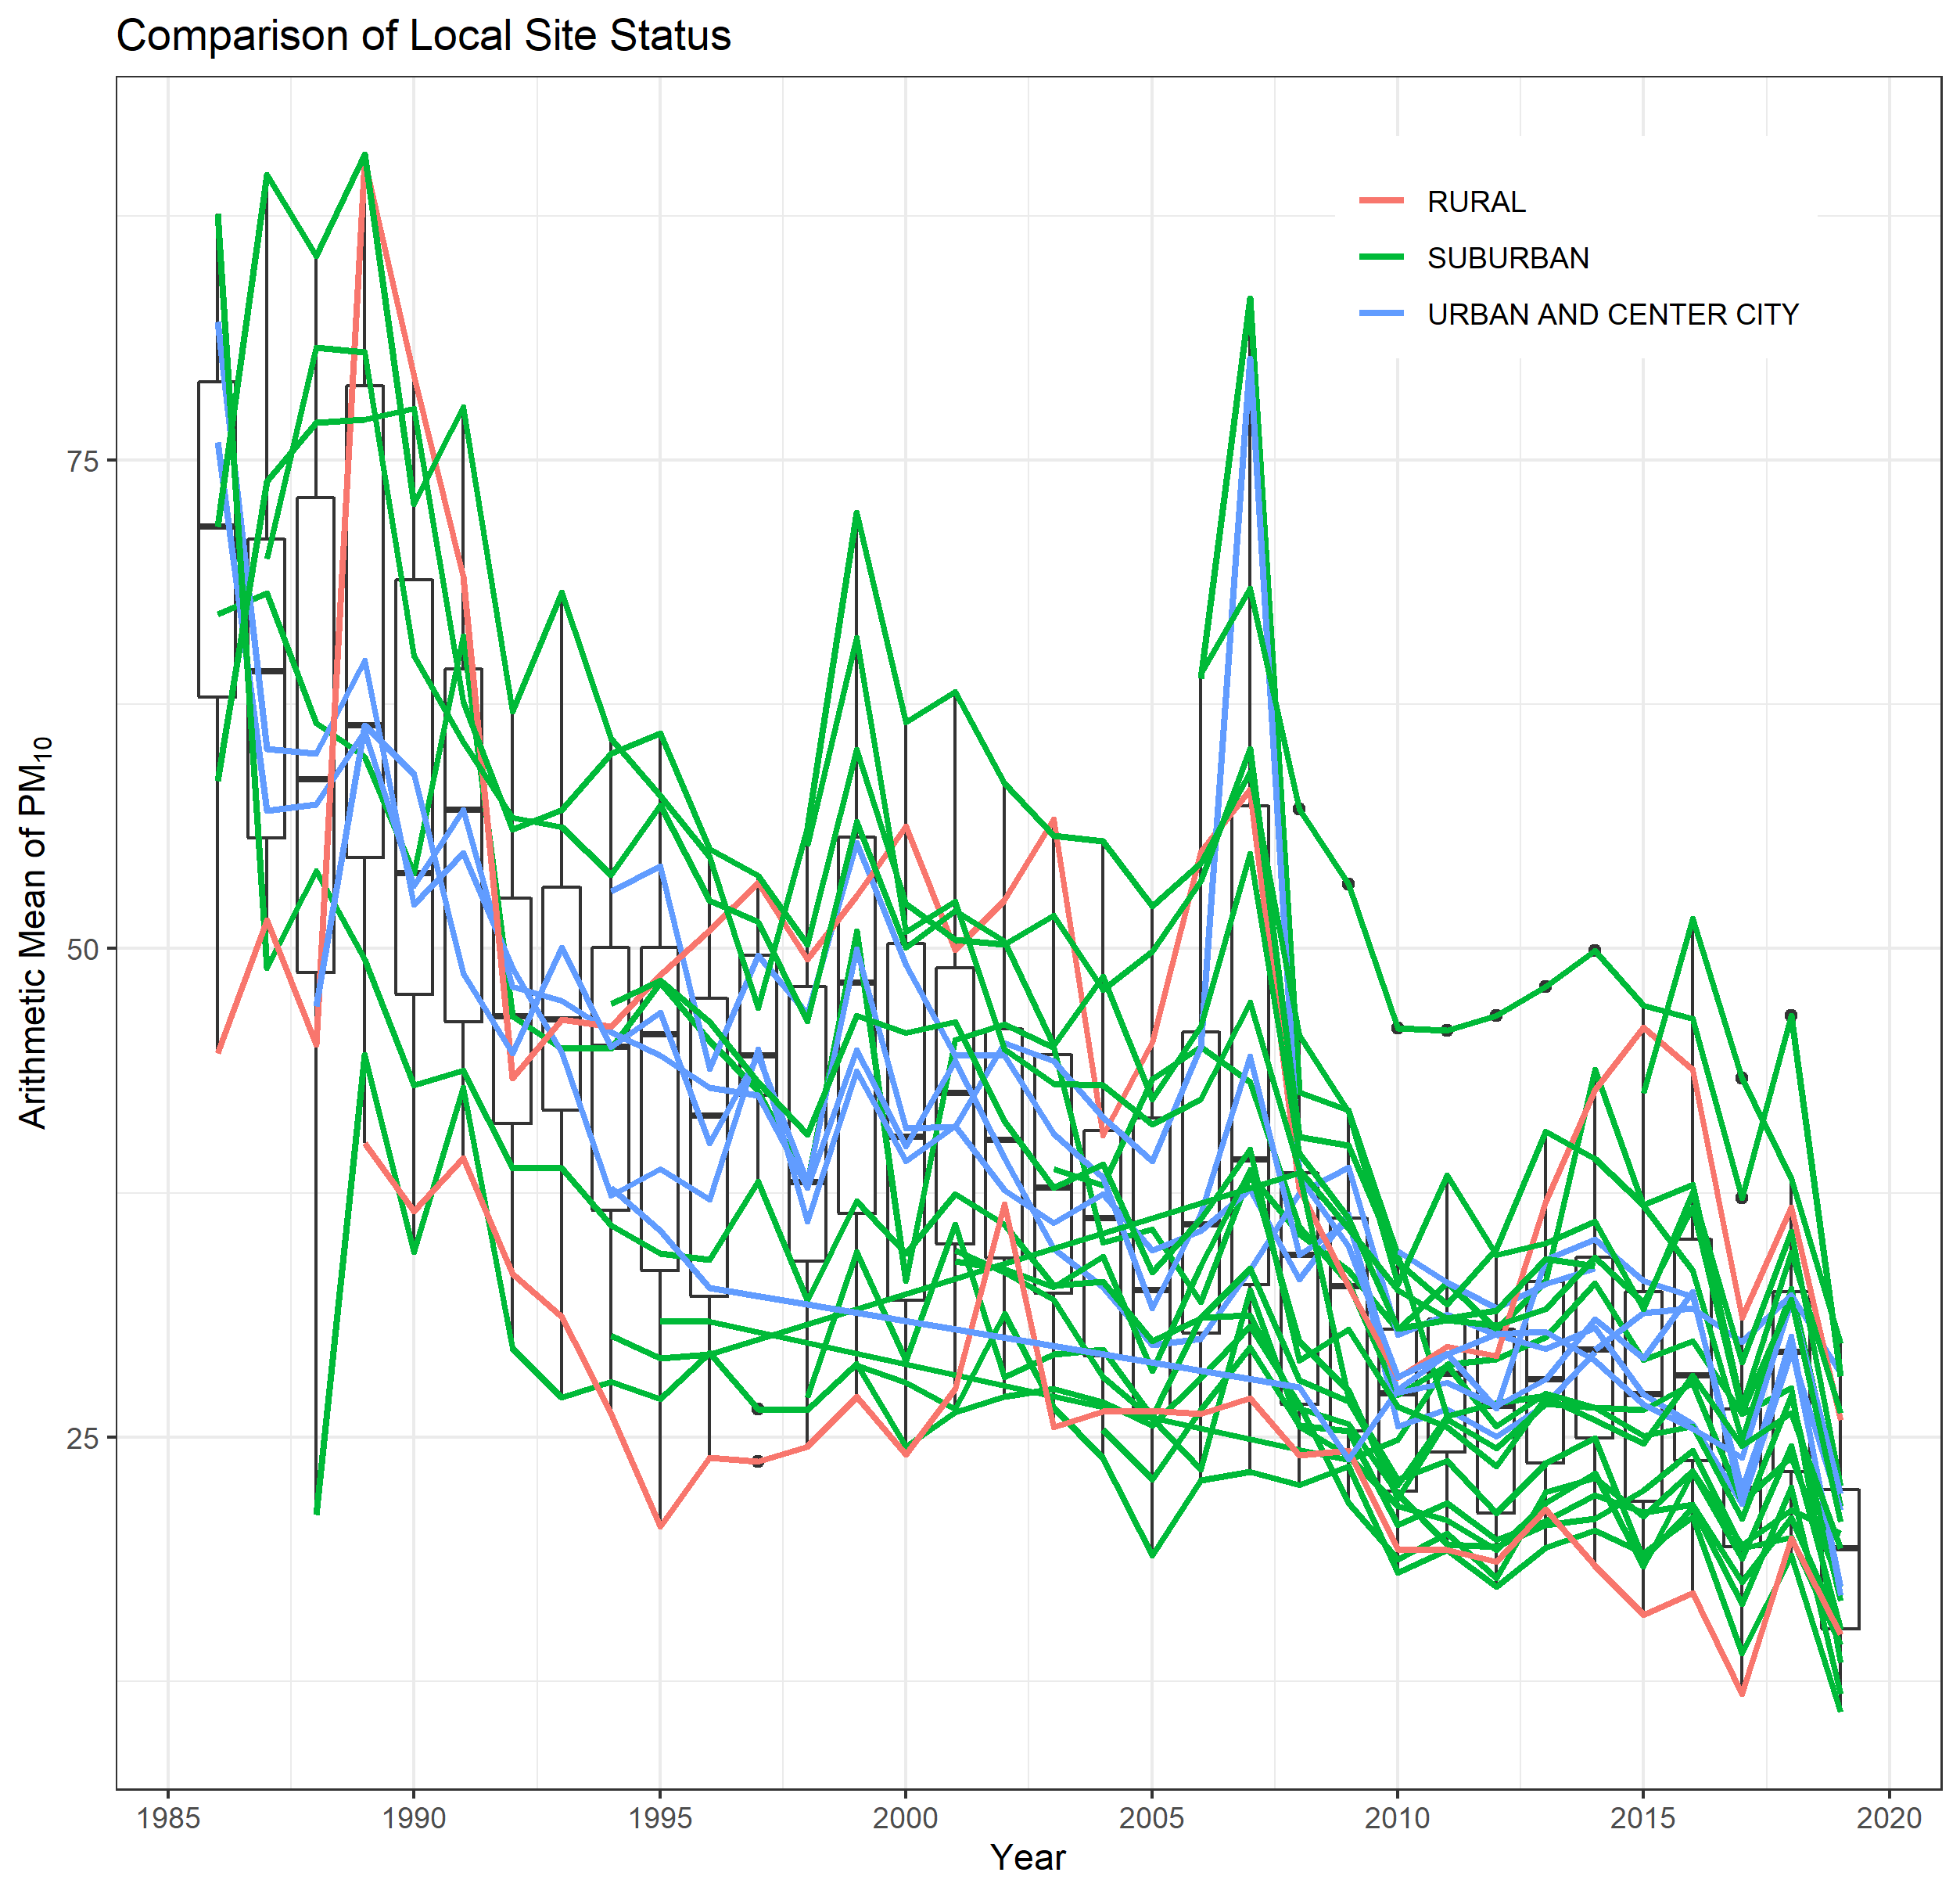
\includegraphics[width = \textwidth]{Figures/SOCAB_metadata_Site_Status.png}
\caption{This shows the site traces coloured by the density of buildings at each site as defined by the EPA.  In the case of multiple \ac{POC}s in at one site, the mean of those \ac{POC}s is taken.  The three categories of sites - Rural (2 sites), Suburban (19 sites), and Urban (7 sites) - are distributed in a way that suggests deliberate choice. Each category seems to be evenly split to have sites above and below the mean.  Urban sites are closely clustered around the overall mean, Suburban generally surround the Urban sites, and the two Rural sites are relatively extreme.  }
\label{fig:SOCAB_metadata_Site_Status}
\end{figure}

\begin{figure}[ht]
\centering
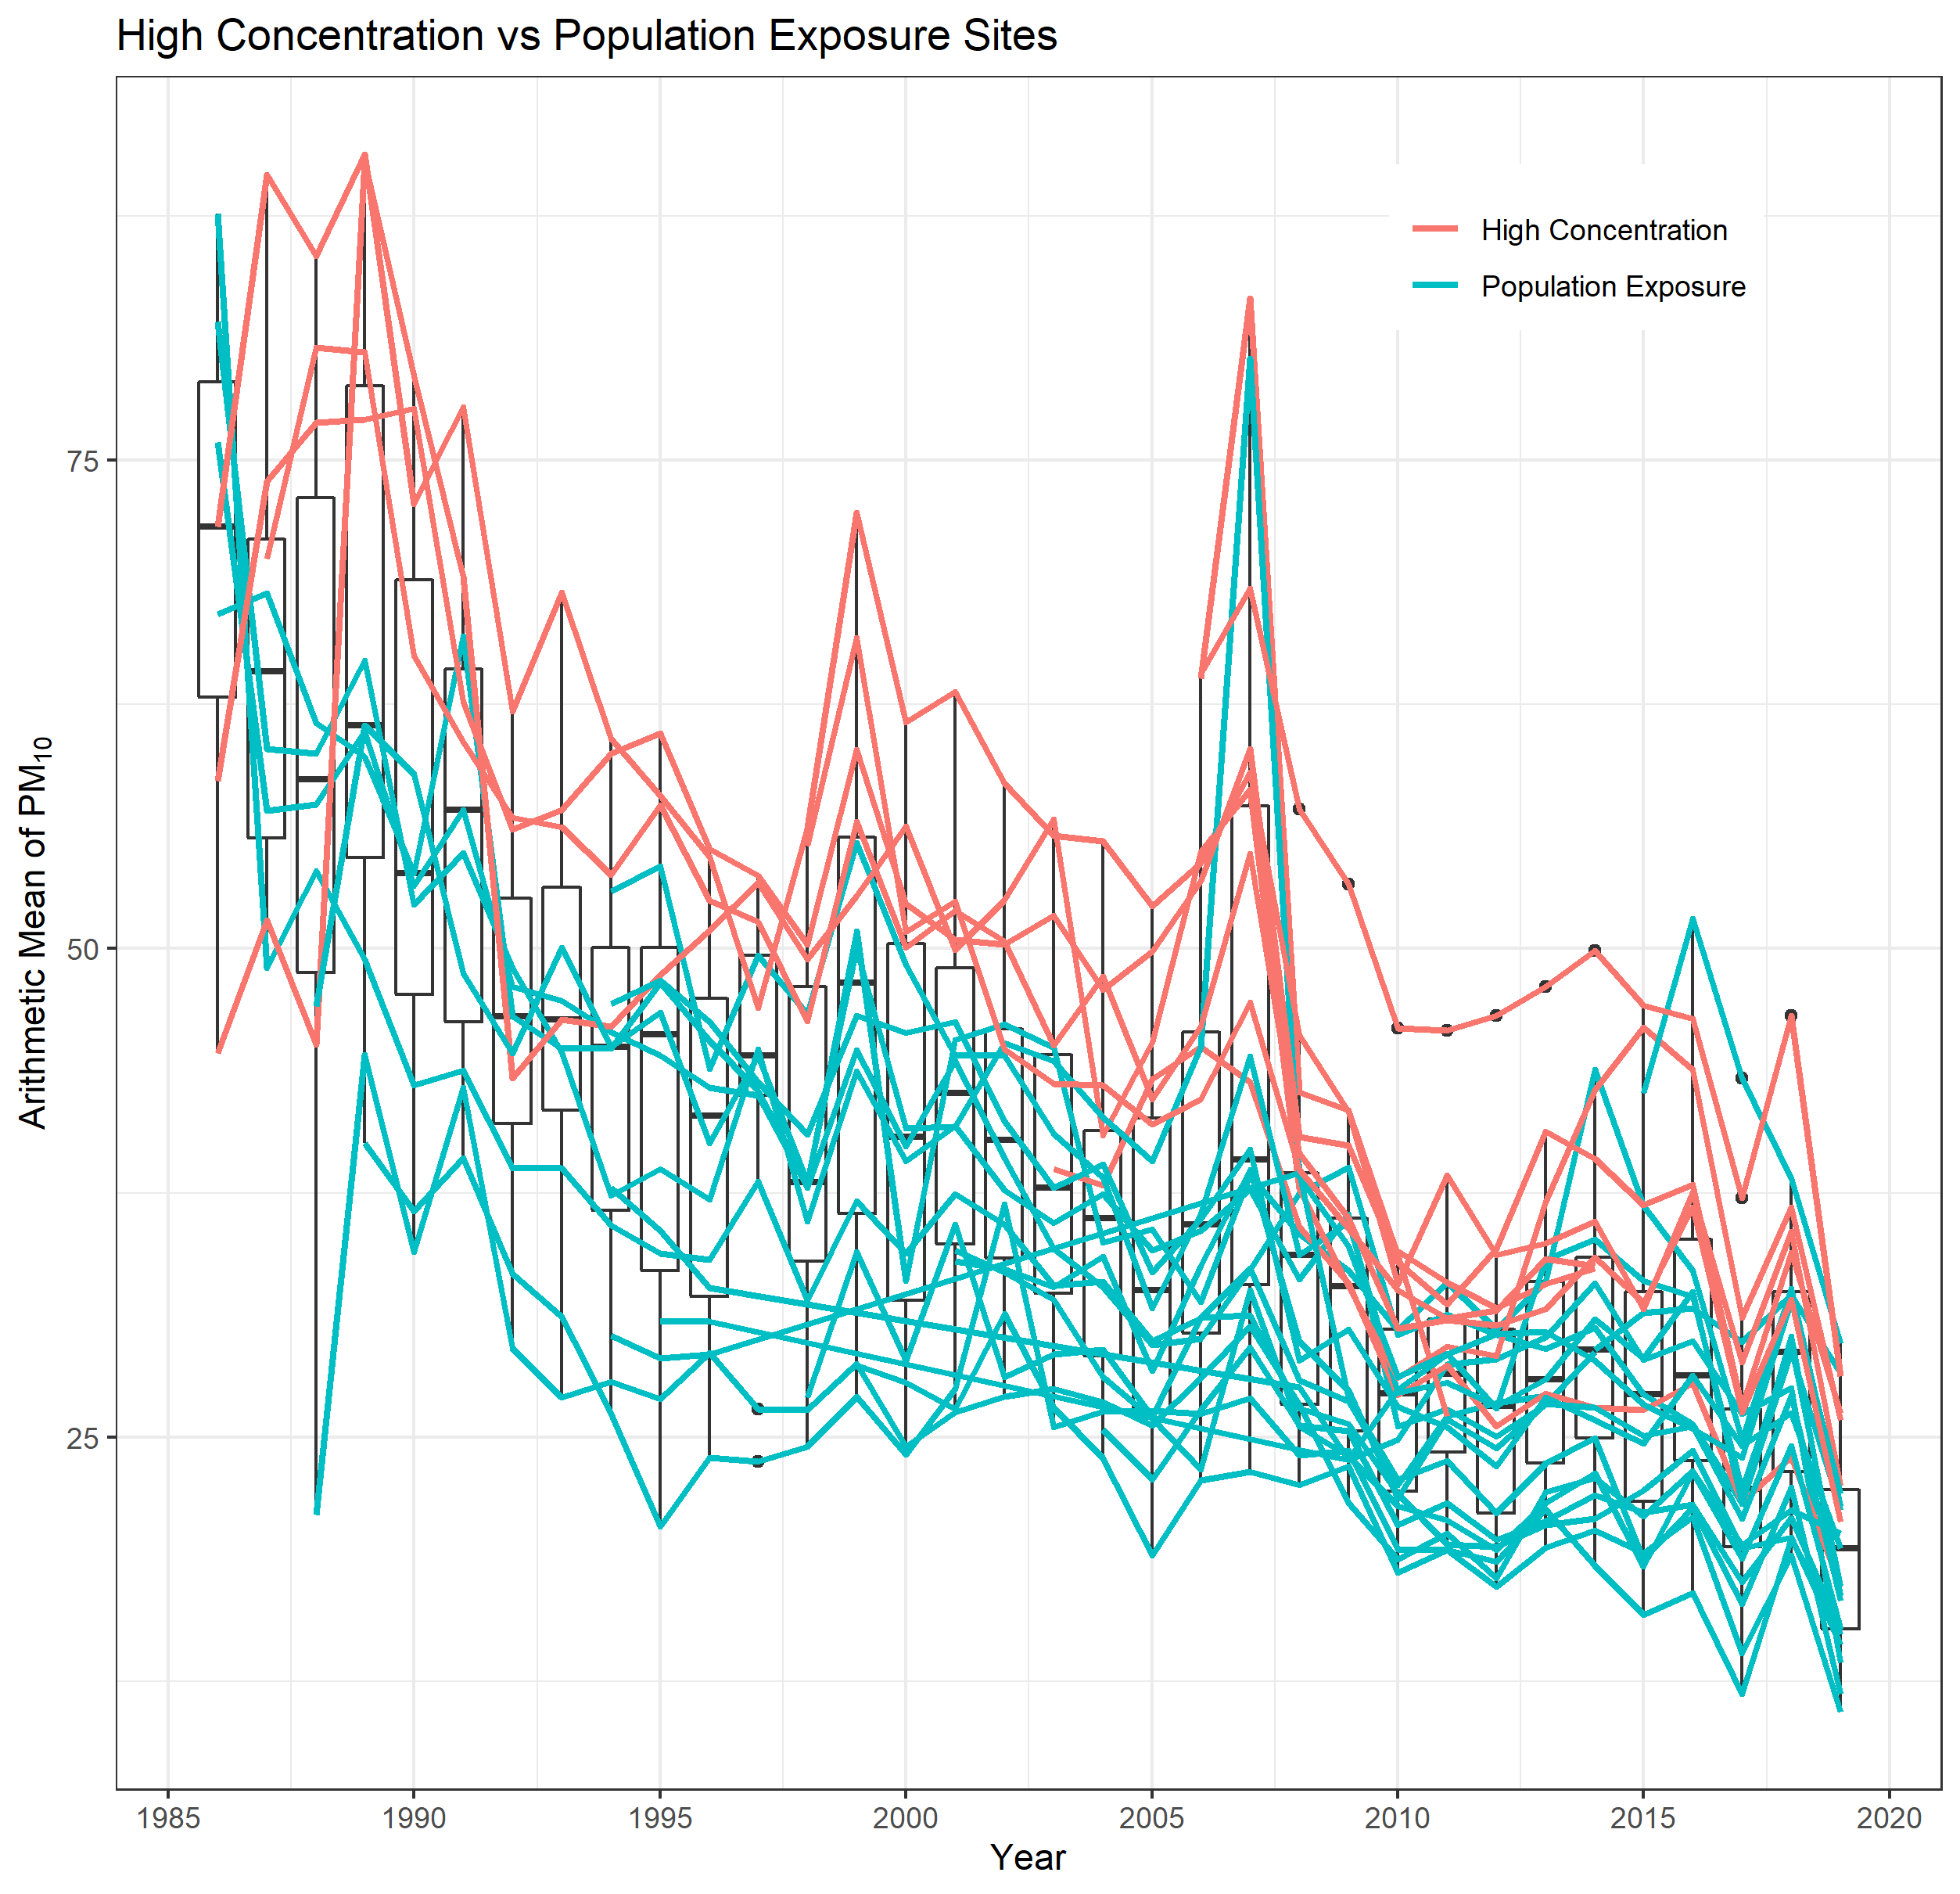
\includegraphics[width = \textwidth]{Figures/SOCAB_metadata_Site_Type.png}
\caption{This shows the site traces coloured by the Site Type category pulled from the \ac{SCAQMD} 5-year reports.  In the case of multiple \ac{POC}s in at one site, the mean of those \ac{POC}s is taken.  On the rare occasion that a site had a different type in 2010 and 2015 or between \ac{FEM} and \ac{FRM} monitors, the most consistent type was used for that site.  The sites designated High Concentration (9 total) are observing a higher concentration than the sites designated Population Exposure (19 total).  }
\label{fig:SOCAB_metadata_Site_Type}
\end{figure}

\subsection{Traditional Spatial Modeling}
\label{subsec:tradspatmod}
Initial spatial modelling using Kriging with a Mat\'{e}rn covariance function examined each year's variogram independently of other years. These produced inconsistent results.  Each year's fitted covariance had different parameters.  Some possible reasons for this are:
\begin{itemize}
\item An insufficient number of sites in a single year leads to instability or non-identifiability in the model.  We think this could be contributing to poor models in the early years.
\item The sites are too far apart to resolve most of the curve of the covariance function. Since \cite{cameletti2011spatio} found a range of 275 km for \ac{PM10} this seems unlikely to be an issue at the scale of the \ac{SOCAB}.
\item Biased sampling makes the estimate of the empirical variogram unreliable, with the bias in the semivariance's estimate increasing with $u$ \citep{diggle:07}.  If, as suspected, there is preferential sampling in the \ac{SOCAB} this could be another reason that the semivariograms did not work well.
\end{itemize}

Variogram plots for each year and their parameter values are not 
included for brevity, 
%can be found in Appendix C, 
but here are three examples demonstrating the range of success in modelling the variograms: Figure \ref{fig:Variogram_1986}, Figure \ref{fig:Variogram2013}, and Figure \ref{fig:Variogram2019}.  Figure  \ref{fig:Variogram_1986} does not have enough sites to make a clear variogram.  Figure  \ref{fig:Variogram2013} has plenty of sites, but exhibits a strange behaviour with raised semivariance at a short range that tails off at a longer range.  Finally, Figure  \ref{fig:Variogram2019} exhibits a nice behaviour with a rise in semivariance over the closer distances and then a rough flattening as the range increases.  

\begin{figure}[ht]
\centering
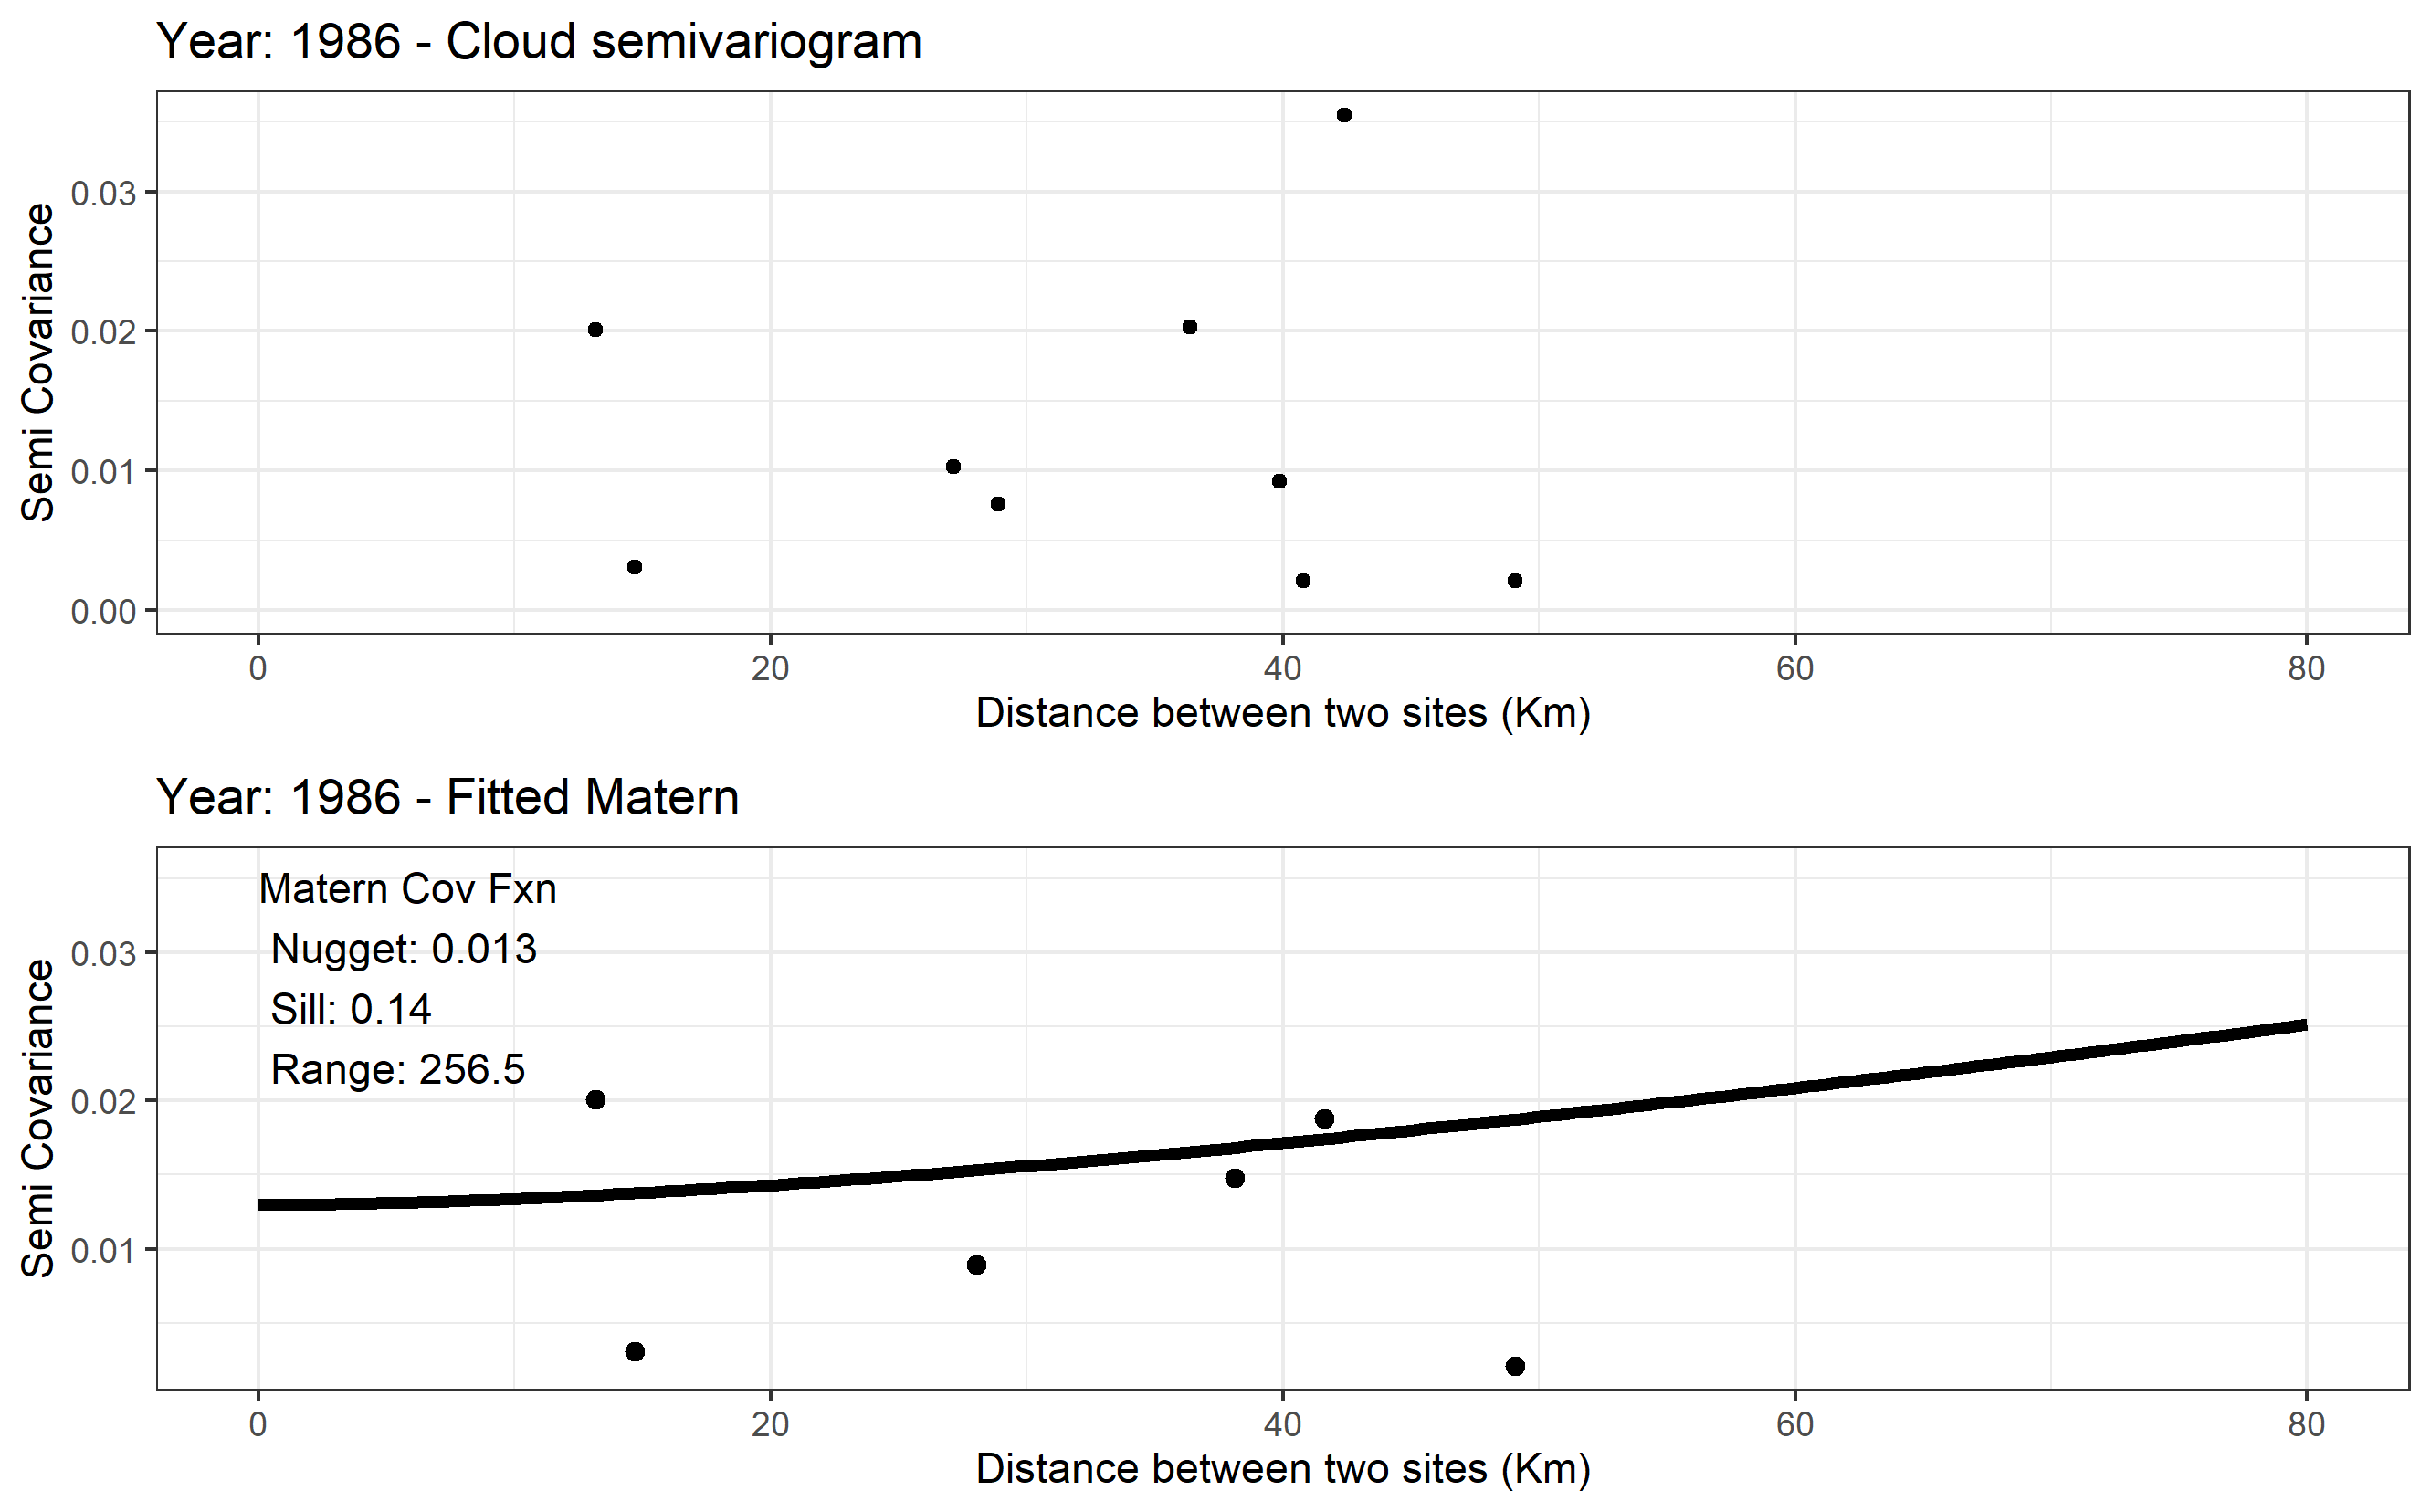
\includegraphics[width = 12cm]{Figures/EmpiricalVariograms/Empirical_Variogram_1986.png}
\caption{At the start of the network, a lack of sites poses a challenge to obtain a sufficient resolution to resolve a fitted variogram.}
\label{fig:Variogram_1986}
\end{figure}

\begin{figure}[ht]
\centering
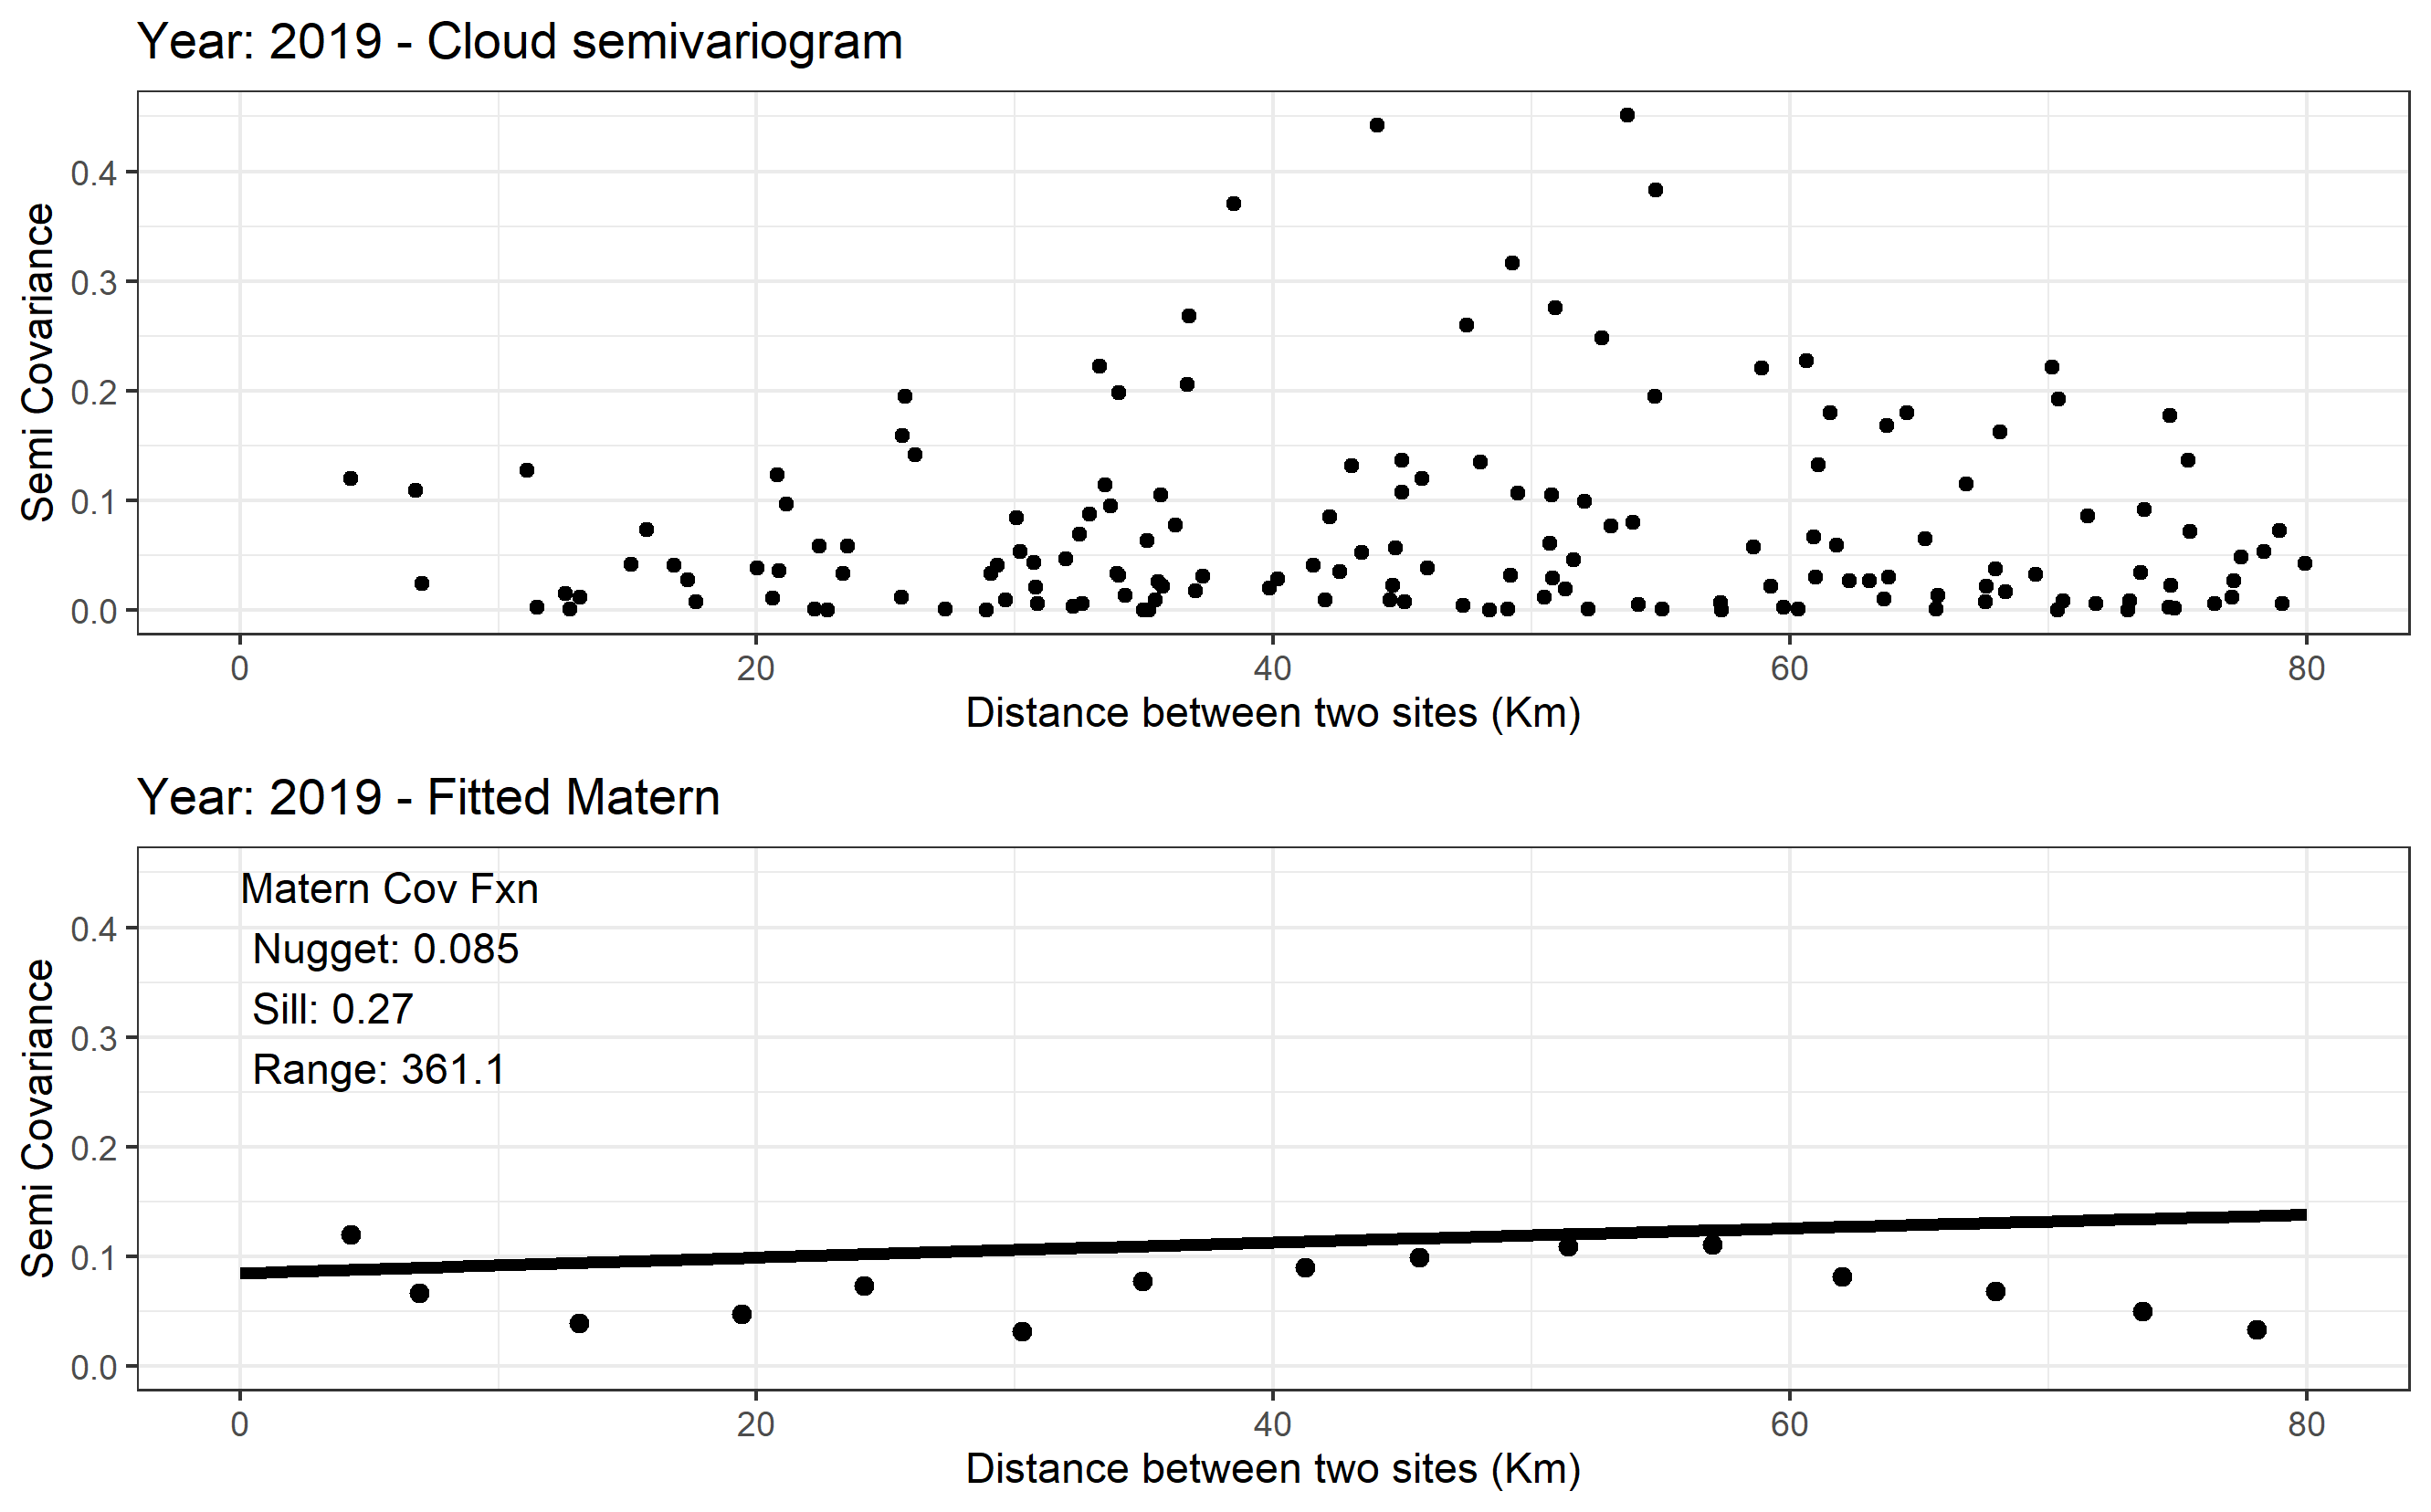
\includegraphics[width = 12cm]{Figures/EmpiricalVariograms/Empirical_Variogram_2019.png}
\caption{Even in later years, there was no guarantee of a good fit.  Here the variogram has no clear trend early on, preventing the curve from being established.}
\label{fig:Variogram2019}
\end{figure}

\begin{figure}[ht]
\centering
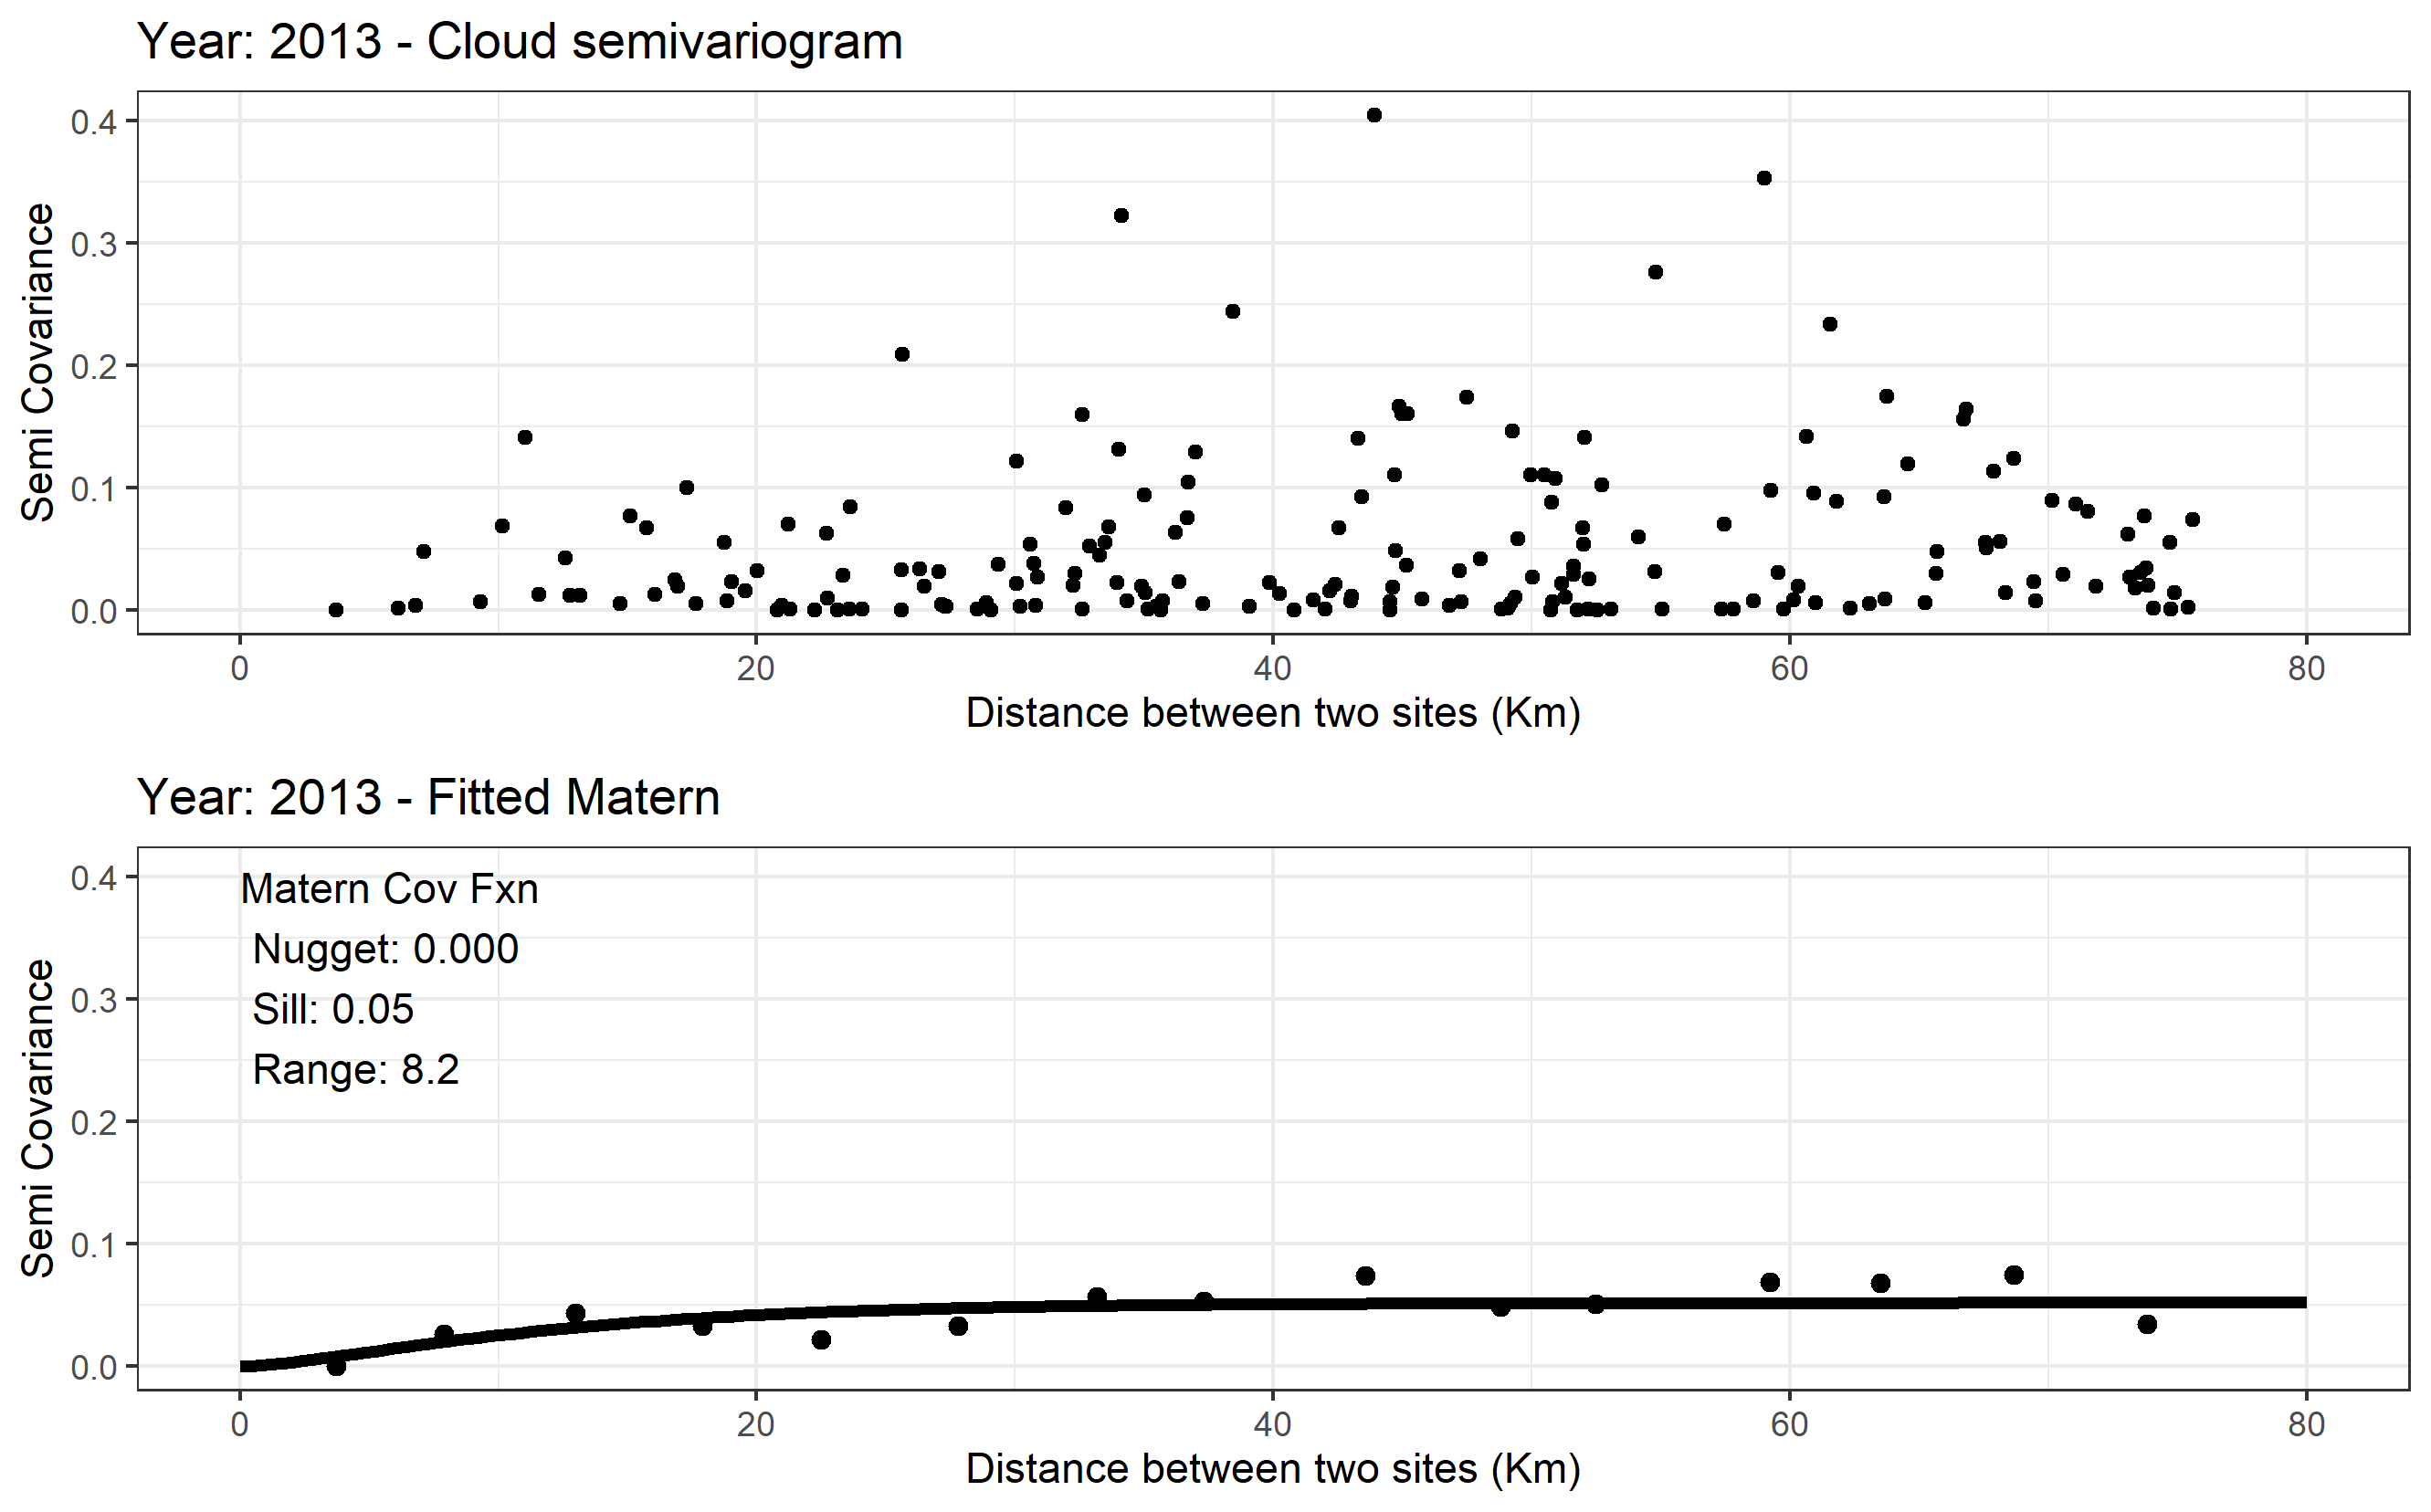
\includegraphics[width = 12cm]{Figures/EmpiricalVariograms/Empirical_Variogram_2013.png}
\caption{Here is one of the better-fitting years.  Key to the success of these types is the small distance estimates having a lower semivariance than most of the rest of the sites.}
\label{fig:Variogram2013}
\end{figure}
